\documentclass[a4paper,twoside,titlepage,11pt]{book}
\usepackage[cm-default]{fontspec}

%ams packages for aling enviroment
\usepackage{amsmath}
\usepackage{amsfonts}
\usepackage{amssymb}
\usepackage[bottom]{footmisc}
%headers
\usepackage{fancyhdr}
\renewcommand{\headrulewidth}{2pt}

%footnote counter reset per page
\usepackage{perpage} %the perpage package
\MakePerPage{footnote} %the perpage package command

% internal hyperlinks
\usepackage{hyperref}
\hypersetup{
    colorlinks,
    citecolor=black,
    filecolor=black,
    linkcolor=black,
    urlcolor=black
}

	\usepackage{multirow}
\usepackage[top=1in,bottom=1in,left=1.4in,right=1.4in]{geometry}

% Pictures
\usepackage{graphicx}
\usepackage{caption}
\usepackage{subcaption}

%hyphenation
%\usepackage{xgreek}
\usepackage[english,greek]{babel}
\usepackage{csquotes}
\renewcommand\thesubfigure{\roman{subfigure}}
%references
\usepackage[backend=bibtex,sorting=none]{biblatex}
\addbibresource{./chapters/references.bib}
\begin{document}
\title{
\vspace{-6ex}
\begin{center}

\includegraphics[scale=0.15]{logo.png}
\end{center}
\Large{Ε}\large{ΘΝΙΚΟ}
\Large{Μ}\large{ΕΤΣΟΒΙΟ}
\Large{Π}\large{ΟΛΥΤΕΧΝΕΙΟ} \\
\normalsize{Τ}\small{ΜΗΜΑ}
\normalsize{Η}\small{ΛΕΚΤΡΟΛΟΓΩΝ}
\normalsize{Μ}\small{ΗΧΑΝΙΚΩΝ}
\normalsize{Κ}\small{ΑΙ}
\normalsize{Μ}\small{ΗΧΑΝΙΚΩΝ}
\normalsize{Υ}\small{ΠΟΛΟΓΙΣΤΩΝ} \\
\vspace{2ex}
ΤΟΜΕΑΣ ΤΕΧΝΟΛΟΓΙΑΣ ΠΛΗΡΟΦΟΡΙΚΗΣ ΚΑΙ ΥΠΟΛΟΓΙΣΤΩΝ \\
ΕΡΓΑΣΤΗΡΙΟ ΥΠΟΛΟΓΙΣΤΙΚΩΝ ΣΥΣΤΗΜΑΤΩΝ \\
\vspace{8ex}
\large \textbf{Πρόβλεψη χρόνου επικοινωνίας παράλληλων εφαρμογών σε αρχιτεκτονικές κοινού χώρου διευθύνσεων} \\
\vspace{10ex}
\large
ΔΙΠΛΩΜΑΤΙΚΗ ΕΡΓΑΣΙΑ \\
\vspace{2ex}
\normalsize
του \\
\vspace{2ex}
\parbox[c]{0.8\textwidth} { \center\textbf{
Παναγιώτη Χ. Μουλλωτού }}
\vspace{10ex}
\flushleft	
\begin{tabbing}
	\textbf{Επιβλέπων}: \= Γεώργιος Ι. Γκούμας \\
			    \> Λέκτορας
\end{tabbing}
}
\date{
\normalsize
Αθήνα, Ιούλιος 2016}

\maketitle
\pagestyle{empty}
\newpage
\frontmatter

\hspace{10pt}
%\tiny
%(this page is left intentionally blanc)
%\normalsize
%\newpage
\frontmatter
\setcounter{page}{1}
\pagestyle{plain}
\hspace{10pt}
\begin{center}

\includegraphics[scale=0.15]{logo.png}

\Large{Ε}\large{ΘΝΙΚΟ}
\Large{Μ}\large{ΕΤΣΟΒΙΟ}
\Large{Π}\large{ΟΛΥΤΕΧΝΕΙΟ} \\
\normalsize{Τ}\small{ΜΗΜΑ}
\normalsize{Η}\small{ΛΕΚΤΡΟΛΟΓΩΝ}
\normalsize{Μ}\small{ΗΧΑΝΙΚΩΝ}
\normalsize{Κ}\small{ΑΙ}
\normalsize{Μ}\small{ΗΧΑΝΙΚΩΝ}
\normalsize{Υ}\small{ΠΟΛΟΓΙΣΤΩΝ} \\
\vspace{2ex}
ΤΟΜΕΑΣ ΤΕΧΝΟΛΟΓΙΑΣ ΠΛΗΡΟΦΟΡΙΚΗΣ ΚΑΙ ΥΠΟΛΟΓΙΣΤΩΝ \\
ΕΡΓΑΣΤΗΡΙΟ ΥΠΟΛΟΓΙΣΤΙΚΩΝ ΣΥΣΤΗΜΑΤΩΝ \\
\end{center}
\begin{center}
\vspace{8ex}
\large \textbf{Πρόβλεψη χρόνου επικοινωνίας παράλληλων εφαρμογών σε αρχιτεκτονικές κοινού χώρου διευθύνσεων} \\
\vspace{10ex}
\large
ΔΙΠΛΩΜΑΤΙΚΗ ΕΡΓΑΣΙΑ \\
\vspace{2ex}
\normalsize
του\\
\vspace{2ex}
\parbox[c]{0.8\textwidth} { \center\textbf{
Παναγιώτη Χ. Μουλλωτού }}
\vspace{10ex}
\flushleft
\begin{tabbing}
	\textbf{Επιβλέπων}: \= Γεώργιος Ι. Γκούμας \\
			    \> Λέκτορας
\end{tabbing}
\end{center}

\noindent
Εγκρίθηκε από την τριμελή εξεταστική επιτροπή την 20$^\eta$ Ιουλίου 2016.\\[1cm]

\begin{center}
\scriptsize
\parbox[b]{0.3\textwidth} {\center
	........................................
	Γεώργιος Γκούμας\\
	Λέκτορας
}
\parbox[b]{0.3\textwidth} {\center
	........................................
	Νεκτάριος Κοζύρης\\
	Καθηγητής
}
\parbox[b]{0.3\textwidth} {\center
	........................................
	Παναγιώτης Τσανάκας\\
	Καθηγητής
}
\end{center}
\vspace{10ex}
\normalsize
\noindent
\begin{center}
Αθήνα, Ιούλιος 2016.
\end{center}
\newpage
\hspace{10pt}

\vspace{20ex}
	\noindent
................................... \\
\textbf{Παναγιώτης Χ. Μουλλωτού} \\
Διπλωματούχος Ηλεκτρολόγος Μηχανικός και Μηχανικός Υπολογιστών Ε.Μ.Π. \\

\vspace*{\fill}
\noindent Copyright\textcopyright \quad  Παναγιώτης Μουλλωτού, 2016\\
Με επιφύλαξη παντός δικαιώματος. All rights reserved.
\paragraph{}
Απαγορεύεται η αντιγραφή, αποθήκευση και διανομή της παρούσας εργασίας, εξ' ολοκλήρου ή τμήματος αυτής, για εμπορικό σκοπό. Επιτρέπεται η  ανατύπωση, αποθήκευση και διανομή για σκοπό μη κερδοσκοπικό, εκπαιδευτικής ή ερευνητικής φύσης, υπό την προϋπόθεση να αναφέρεται η πηγή προέλευσης και να διατηρείται το παρόν μήνυμα. Ερωτήματα που αφορούν τη χρήση της εργασίας για κερδοσκοπικό σκοπό πρέπει να απευθύνονται προς το συγγραφέα.
\paragraph{}
Οι απόψεις και τα συμπεράσματα που περιέχονται σε αυτό το έγγραφο εκφράζουν τον συγγραφέα και δεν πρέπει να ερμηνευθεί ότι αντιπροσωπεύουν τις επίσημες θέσεις του Εθνικού Μετσόβιου Πολυτεχνείου.  
\newpage


\section*{\centering Περίληψη}
\addcontentsline{toc}{chapter}{Περίληψη}
Με τη δουλειά μας, παρουσιάζουμε μία μεθοδολογία για την πρόβλεψη του χρόνου επικοινωνίας παράλληλων εφαρμογών σε αρχιτεκτονικές κοινής μνήμης βασιζόμενοι σε τεχνικές μηχανικής μάθησης, για σημείο-προς-σημείο αλλά και συλλογική επικοινωνία, που παρέχει το προγραμματιστικό μοντέλο ανταλλαγής μηνυμάτων, MPI.  Χρησιμοποιούμε διάφορα benchmarks για την εξαγωγή ενός συνόλου με σημεία-παραδείγματα. Κάθε σημείο περιέχει κάποια χαρακτηριστικά που αποτυπώνουν την επικοινωνία που λαμβάνει χώρα και το χρόνο επικοινωνίας που δαπανήθηκε. Μετέπειτα, στηριζόμενοι στα σημεία επικοινωνίας που εξάγαμε, εκπαιδεύουμε τα μοντέλα με αλγόριθμους επιτηρούμενης μάθησης και αξιολογούμε τη συμπεριφορά τους για διάφορα σύνολα δειγμάτων εκπαίδευσης, με τη βοήθεια δύο MPI εφαρμογών, Jacobi και LULESH, και διάφορων μετρικών αξιολόγησης. Τελικά, τα αποτελέσματα για επικοινωνία σημείο-προς-σημείο παρουσιάζουν αξιοσημείωτη ακρίβεια με τουλάχιστον 75\%  των περιπτώσεων που προβλέπουμε να έχουν απόλυτο σχετικό σφάλμα μικρότερο από 30\% για όλες τις αρχιτεκτονικές που εξετάσαμε. Αντίστοιχης κλίμακας ακρίβεια παρουσιάζουν οι προβλέψεις συλλογικής επικοινωνίας. Επιπρόσθετα,  πέραν των προβλέψεων, αναλύουμε τις προκλήσεις που εμφανίζει η μελέτη της συλλογικής επικοινωνίας.

\vspace*{\fill}
\textbf{Λέξεις-κλειδιά:} χρόνος επικοινωνίας, MPI εφαρμογές, αρχιτεκτονικές κοινής μνήμης, μηχανική μάθηση
\newpage

\section*{\centering Abstract}

\addcontentsline{toc}{chapter}{Abstract}
\selectlanguage{english}
In this paper, we represent a  methodology aiming to predict the time consumed by parallel applications for communication purposes, based on machine learning technics, applicable for point-to-point and collective MPI operations. We use several benchmarks in order to extract a training set containing samples. Each sample is formed by a number of features, grasping the communication that took place during the benchmarks' execution, followed by the time consumed. Afterwards, we implement supervised learning algorithms for the models' training and we evaluate their accuracy for two modern MPI applications, Jacobi and LULESH. Finally, point-to-point operations are predicted with noteworthy results by combining the samples extracted from two benchmarks, acheiving absolute relative error below 25\% while scoring higher than 75\% in $Pred_{0.3}$. Moreover, except for making predictions, we analyse the challenges presented by collective operations modeling.

\vspace*{\fill}
\textbf{Keywords:} communication time, MPI application, shared memory architectures, machine learning,
\newpage
\section*{\centering Ευχαριστίες}
\selectlanguage{greek}
\addcontentsline{toc}{chapter}{Ευχαριστίες}
\paragraph{}
Αρχικά θέλω να ευχαριστήσω τον επιβλέποντα καθηγητή μου κ. Γεώργιο Γκούμα για την ανάθεση αυτής της Διπλωματικής και την βοήθεια που μου έδωσε κατά τη διάρκεια της εκπόνησής της. Πάνω απ΄όλα τον ευχαριστώ γιατί αποτέλεσε τον κύριο λόγο για να ασχοληθώ με την επιστήμη υπολογιστών και τα παράλληλα συστήματα.
\paragraph{}
Ένα μεγάλο ευχαριστώ οφείλω στην υποψήφια διδάκτορα Νικέλα Παπαδοπούλου. Η συνδρομή της ήταν καθοριστική στην ολοκλήρωση της διπλωματικής αυτής, παρέχοντας γνώση, καθοδήγηση και εμπιστοσύνη, με άψογη συνεργασία αυτούς τους τελευταίους μήνες.
\paragraph{}
Επιπλέον, θέλω να ευχαριστήσω τους φίλους και συμφοιτητές μου, για τη βοήθεια και στήριξη που μου παρείχαν στα πέντε χρόνια φοίτησης μου στο Πολυτεχνείο.
\paragraph{}
Τέλος, δεν μπορώ να βρω τις λέξεις για να εκφράσω την ευγνωμοσύνη μου προς τους γονείς μου. Η εμπιστοσύνη και η αλτρουιστική στήριξη τους είναι πραγματικά συγκινητική. Η διπλωματική αυτή είναι αφιερωμένη σε αυτούς.


\newpage
\tableofcontents
{\small\listoffigures}
\mainmatter{
\pagenumbering{arabic}

\pagestyle{fancy}
\fancyhf{}
%\cfoot{\thepage}
\fancyfoot[LE,RO]{\thepage}
\chapter{Εισαγωγή}
\fancyhead[RE,LO]{Εισαγωγή}
\section{Συστήματα Κοινής και Κατανεμημένης Μνήμης}
\paragraph{}
Με βάση την οργάνωση της μνήμης τους, τα πολυπύρηνα συστήματα χωρίζονται σε κοινής μνήμης (shared memory) και κατανεμημένης μνήμης (distributed memory). Στις αρχιτεκτονικές κοινής μνήμης οι επεξεργαστές του συστήματος προσπελαύνουν όλοι την ίδια φυσική μνήμη και τις περισσότερες φορές η διασύνδεσης τους γίνεται μέσω ενός διαδρόμου (memory bus) βλ. Σχήμα \ref{fig:SMP}. Αντίθετα, στις αρχιτεκτονικές κατανεμημένης μνήμης κάθε επεξεργαστής έχει τη δική του ιδιωτική μνήμη, και η επικοινωνία μεταξύ τους γίνεται πάνω από κάποιο δίκτυο διασύνδεσης βλ. Σχήμα  \ref{fig:cluster}.

\begin{figure}
    \centering
    \begin{subfigure}[b]{0.45\textwidth}
        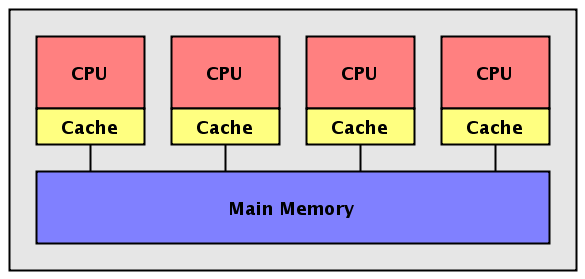
\includegraphics[width=\textwidth]{./images/SMP.png}
        \caption{Κοινής Μνήμης}
        \label{fig:SMP}
    \end{subfigure}
    \quad %add desired spacing between images, e. g. ~, \quad, \qquad, \hfill etc. 
      %(or a blank line to force the subfigure onto a new line)
    \begin{subfigure}[b]{0.45\textwidth}
        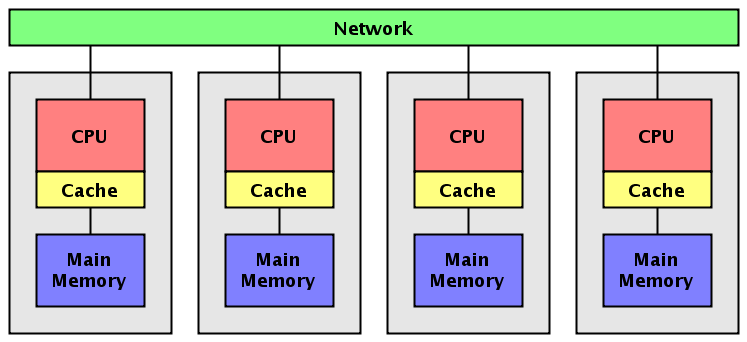
\includegraphics[width=\textwidth]{./images/cluster.png}
        \caption{Κατανεμημένης Μνήμης}
        \label{fig:cluster}
    \end{subfigure}
    \caption{Αναπαράσταση συστημάτων κοινής και κατανεμημένης μνήμης}
\end{figure}
\paragraph{}
Ανάλογα με την οργάνωση τους, οι αρχιτεκτονικές κοινής μνήμης χωρίζονται σε δύο κατηγορίες. Η πρώτη κατηγορία αφορά περιπτώσεις όπου ο χρόνος πρόσβασης στη μνήμη είναι σταθερός και ονομάζεται Ομοιόμορφης Πρόσβασης στη Μνήμη(Uniform Memory Access-UMA). Σε αυτή την περίπτωση ο επεξεργαστής, και το block που προσπελαύνει, δεν επηρεάζουν το χρόνο πρόσβασης στη μνήμη. Στη δεύτερη κατηγορία εμπίπτουν τα συστήματα όπου η κοινή μνήμη είναι κατανεμημένη στους επεξεργαστές και επιπλέον υλικό φροντίζει για την πρόσβαση των επεξεργαστών σε μη τοπικές μνήμες. Είναι προφανές ότι πλέον ο χρόνος πρόσβασης δεν είναι σταθερός. Έτσι τα συστήματα αυτά ονομάζονται Μη-Ομοιόμορφης Πρόσβασης στη Μνήμη(Non-Uniform Memory Access-NUMA). Μία οπτική αναπαράσταση για τις δύο κατηγορίες δίνεται στο Σχήμα \ref{fig:shared_mem}.\footnote{Εικόνες από: www.sqlskills.com/blogs/jonathan/understanding-non-uniform-memory-accessarchitectures-numa}

\begin{figure}
    \centering
    \begin{subfigure}[b]{0.45\textwidth}
        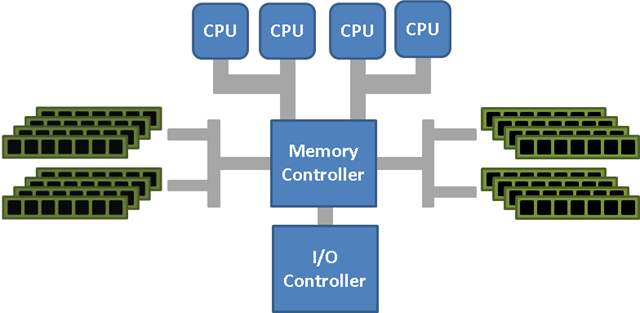
\includegraphics[width=\textwidth]{./images/UMA.png}
        \caption{UMA}
    \end{subfigure}
    \quad %add desired spacing between images, e. g. ~, \quad, \qquad, \hfill etc. 
      %(or a blank line to force the subfigure onto a new line)
    \begin{subfigure}[b]{0.45\textwidth}
        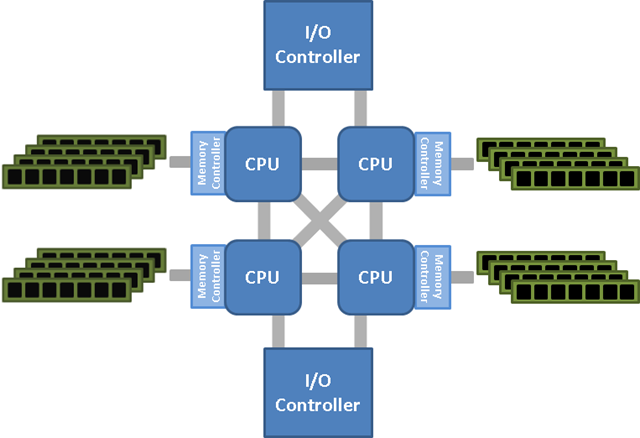
\includegraphics[width=\textwidth]{./images/NUMA.png}
        \caption{NUMA}
    \end{subfigure}
    \caption{Κατηγορίες Αρχιτεκτονικών Κοινής Μνήμης}
    \label{fig:shared_mem}
\end{figure}

\paragraph{}
Οι σύγχρονοι υπερυπολογιστές χρησιμοποιούν συνδυασμούς των δύο παραπάνω δημιουργώντας υβριδικές αρχιτεκτονικές. Συνήθως οι κόμβοι\footnote{Με τον όρο κόμβοι θα αναφερόμαστε στο κομμάτι του συστήματος που είναι συνδεδεμένο στο δίκτυο διασύνδεσης} τους αποτελούνται από εμπορικούς επεξεργαστές, επιταχυντές γραφικών ή co-processors όπως ο Xeon Phi. Καθώς προσεγγίζουμε την εποχή του exascale computing, στην οποία ένας υπερυπολογιστής θα έχει την δυνατότητα να εκτελέσει ένα τρισεκατομμύριο πράξεις κινητής υποδιαστολής το δευτερόλεπτο, οι σχεδιαστές των μηχανημάτων έχουν την τάση να σχεδιάζουν συστήματα στα οποία  κάθε κόμβος έχει πάρα πολλούς <<αδύναμους>> πυρήνες και ακόμα περισσότερα νήματα. Τέσσερις από τους δέκα ισχυρότερους υπολογιστές του κόσμου για το 2015, συνδυάζουν σε κάθε κόμβο ένα απλό επεξεργαστή με αρχιτεκτονική κοινού χώρου διευθύνσεων με ένα co-processor που περιέχει δεκάδες επεξεργαστές. Αυτά τα δύο είναι συνδεδεμένα μεταξύ τους, συνήθως μέσω PCIe, σχηματίζοντας ένα κόμβο που συνδέεται με άλλους μέσω κάποιου εξελιγμένου δικτύου διασύνδεσης 

\paragraph{}
Δύο παραδείγματα υπερυπολογιστών, σε φάση κατασκευής, που υλοποιούν την πιο πάνω υβριδική αρχιτεκτονική είναι ο Theta από το Argonne National Laboratory και ο Cori από το National Energy Research Scientific Computing Center. Και οι δύο χρησιμοποιούν ένα συνδυασμό Intel Xeon με Intel Xeon Phi σε κάθε κόμβο, που τελικά περιέχει πάνω από 70 πυρήνες ή 280 νήματα. Επιπλέον, η τάση αυτή φαίνεται να ενισχύεται, με ιθύνοντες της Intel να υποστηρίζουν ότι ο πρώτος exascale υπολογιστής θα περιέχει χιλιάδες πυρήνες σε κάθε κόμβο\footnote{http://www.nextplatform.com/2015/08/12/future-systems-intel-fellow-conjures-the-perfect-exascale-machine/} με το UC Davis να έχει ήδη αναπτύξει τον πρώτο επεξεργαστή με χίλιους πυρήνες.\footnote{https://www.ucdavis.edu/news/worlds-first-1000-processor-chip}

\paragraph{}
Ωστόσο, το συνονθύλευμα αυτών των αρχιτεκτονικών οδηγεί σε μία περίπλοκη ιεραρχία μνήμης. Κάθε πυρήνας έχει κάποια ιδιωτική  κρυφή μνήμη (cache) για μερικά επίπεδα. Σε επόμενο στάδιο, ανάλογα με τον πυρήνα, μπορεί να υπάρχει κοινό επίπεδο cache για όλους τους πυρήνες που βρίσκονται στον ίδιο επεξεργαστή ή κάποια άλλου είδους επικοινωνία για πυρήνες στο ίδιο package. Στην περίπτωση του Xeon Phi, ένας δακτύλιος δύο κατευθύνσεων συνδέει τους πυρήνες μεταξύ τους και με μνήμη on the package (DDR5 ή custom made). Σε επόμενα επίπεδα συναντάμε την κύρια μνήμη, μνήμες όπως NVRAM και μαγνητικούς σκληρούς δίσκους για μόνιμη αποθήκευση, ενώ στο τελευταίο επίπεδο συνήθως βρίσκουμε μαγνητικές ταινίες που αποσκοπούν σε μακροπρόθεσμη αποθήκευση κυρίως για σκοπούς αντιγράφων ασφαλείας. 

\paragraph{}
Αυτή η βαθιά ιεραρχία μνήμης εισάγει νέες προκλήσεις. Πλέον η θέση της διεργασίας στο μηχάνημα θα είναι όλο και πιο κρίσιμη για την επικοινωνία της. Ανάλογα με τη θέση της διεργασίας που καλείται να ανταλλάξει δεδομένα, διαφορετικά πρότυπα επικοινωνίας θα λαμβάνουν χώρα.

\paragraph{}
Μία από τις προσπάθειες για αντιμετώπιση των προκλήσεων που εμφανίζονται καθώς οδεύουμε στην εποχή του exascale, είναι το Ευρωπαϊκό ερευνητικό πρότζεκτ Exanode. Πρόκειται για την προσπάθεια της επιστημονικής κοινότητας να σχεδιάσει τον ιδανικό κόμβο. Θα είναι βασισμένος στην αρχιτεκτονική του ARM-v8 ενώ θα περιέχει μνήμη που θα υποστηρίζει κλιμακωσιμότητα για τον exascale υπολογιστή. 

\section{Παράλληλα Προγραμματιστικά Μοντέλα}
\paragraph{}
Για κάθε αρχιτεκτονική που αναφερθήκαμε έχουν αναπτυχθεί και ανάλογα προγραμματιστικά μοντέλα. Έτσι έχουμε το μοντέλο κοινού χώρου διευθύνσεων, το μοντέλο ανταλλαγής μηνυμάτων για συστήματα κατανεμημένης μνήμης και το υβριδικό μοντέλο που συνδυάζει τα δύο προηγούμενα. Στόχος τους είναι να παρέχουν στους προγραμματιστές ευκολία στη γραφή κώδικα, χωρίς να τους επιβαρύνουν με λεπτομέρειες της υλοποίησης αλλά ταυτόχρονα να εκμεταλλεύονται όσο το δυνατό περισσότερο τα πλεονεκτήματα και τα χαρακτηριστικά της κάθε αρχιτεκτονικής.
\subsection{Μοντέλο κοινού χώρου διευθύνσεων}
\paragraph{}
Το μοντέλο αυτό είναι σχεδιασμένο για αρχιτεκτονικές κοινού χώρου διευθύνσεων. Καθώς όλες οι διεργασίες έχουν πρόσβαση στην ίδια μνήμη, η επικοινωνία μεταξύ τους γίνεται ασύγχρονα μέσω πρόσβασης σε κοινές θέσης μνήμης. Ωστόσο, ταυτόχρονες προσβάσεις στην ίδια θέση μνήμης ενδέχεται να δημιουργήσουν καταστάσεις ανταγωνισμού (race conditions), με τη χρήση σχημάτων συγχρονισμού να είναι απαραίτητη. Πρόκειται αδιαμφισβήτητα για το πιο απλό μοντέλο από προγραμματιστική σκοπιά, με τις εκάστοτε υλοποιήσεις να αναλαμβάνουν να επιλύσουν θέματα συγχρονισμού. Υπάρχουν ποικίλες υλοποιήσεις του μοντέλου (OpenMP, Cilk, Thread Building Blocks) με την πιο ευρέως διαδεδομένη την OpenMP.

\subsection{Μοντέλο Ανταλλαγής Μηνυμάτων}
\paragraph{}
Το μοντέλο αυτό αποσκοπεί στην υλοποίηση της επικοινωνίας μεταξύ διεργασιών όπου η μνήμη του συστήματος είναι κατανεμημένη. Οι διεργασίες επικοινωνούν μεταξύ τους ανταλλάσσοντας μηνύματα μέσω ποικίλων εντολών. Η κλήση των εντολών γίνεται από τον προγραμματιστή, δίνοντας του έτσι την ευχέρεια να ορίσει ποιες διεργασίες θα επικοινωνήσουν, τα δεδομένα που θα ανταλλάξουν και σε ποιο στάδιο της εκτέλεσης να θα γίνει επικοινωνία. Στην πιο απλή μορφή της, μια εντολή με σκοπό την αποστολή δεδομένων περιλαμβάνει τη διεύθυνση ενός τοπικού buffer με τα δεδομένα, το αναγνωριστικό της διεργασίας-παραλήπτη και τον τύπο των δεδομένων που αποστέλνονται. Αναλογικά, μία εντολή λήψης δεδομένων, περιλαμβάνει ένα buffer για την αποθήκευση των εισερχόμενων δεδομένων, το αναγνωριστικό της διεργασίας-αποστολέα και τον τύπο των δεδομένων που παραλαμβάνονται.


\paragraph{}
Επιπλέον, το μοντέλο ανταλλαγής μηνυμάτων υποστηρίζει διάφορα είδη επικοινωνίας. Ένα είδος είναι η σύγχρονη (blocking) όπου οι διεργασίες συγχρονίζονται κατά την αποστολή των δεδομένων. Ουσιαστικά, με την κλήση των συναρτήσεων send, από τη διεργασία-αποστολέα, και receive, από τη διεργασία-παραλήπτη,  οι διεργασίες αναστέλλουν τη λειτουργία τους εώς το πέρας της επικοινωνίας. Αντίθετα, στην ασύγχρονη επικοινωνία (non-blocking) οι κλήσεις send και receive επιστρέφουν όσο το δυνατό γρηγορότερα, έχοντας αναθέσει την αποστολή και λήψη των δεδομένων σε κάποιο άλλο μηχανισμό, χωρίς η επικοινωνία να έχει ολοκληρωθεί. Σε επόμενο στάδιο, κάποια συνάρτηση τύπου wait καλείται πριν κάποια από τις διεργασίες προσπελάσει τα νέα δεδομένα για να διασφαλιστεί ότι έχουν ληφθεί. Αν το υλικό το επιτρέπει και οι μηχανισμοί που αναλαμβάνουν την αποπεράτωση της διαδικασίας είναι ανεξάρτητοι από την εκτέλεση της διεργασίας, η non-blocking επικοινωνία επιτρέπει σε υπολογισμούς και επικοινωνία να γίνουν ταυτόχρονα. 

\paragraph{}
Μία άλλη διάκριση μεταξύ των ειδών επικοινωνίας είναι η σημείο-προς-σημείο (point-to-point) και η συλλογική επικοινωνία (collectives). Στην επικοινωνία point-to-point συμμετέχουν μόνο δύο διεργασίες, μία που αποστέλλει και μία που λαμβάνει δεδομένα. Στα collectives μπορούν να λαμβάνουν μέρος περισσότερες από δύο διεργασίες. Τέτοιου είδους επικοινωνία είναι συνηθισμένη όταν μια διεργασία καλείται να αποστείλει δεδομένα σε πολλές διεργασίες ή αντίθετα, να λάβει δεδομένα από διάφορες διεργασίες.

\paragraph{}
Υπάρχουν επίσης, πολλές υλοποιήσεις αυτού του προγραμματιστικού μοντέλου, με τις περισσότερες να ακολουθούν το πρότυπο MPI(Message Passing Interface) που αναπτύσσεται από το MPI forum \cite{MPI}. Το πρότυπο αυτό καθορίζει τις λειτουργίες που πρέπει να προσφέρει μία υλοποίηση του μοντέλου. Διασημότερες υλοποιήσεις είναι το OpenMPI \cite{OMPI} και το MPICH \cite{MPICH}. Στα πειράματα μας επιλέξαμε να χρησιμοποιήσουμε το OpenMPI, καθώς ενσωματώνει νέα χαρακτηριστικά πολύ γρήγορα και παραμένει σε μεγάλο βαθμό ερευνητικό εργαλείο.
\subsection{Υβριδικό Μοντέλο}
Στις περισσότερες εφαρμογές που προορίζονται για εκτέλεση σε υπερυπολογιστές, χρησιμοποιείται το υβριδικό μοντέλο, που συνδυάζει MPI με κάποια υλοποίηση του μοντέλου κοινού χώρου διευθύνσεων. Για επικοινωνία μεταξύ των διεργασιών που βρίσκονται στον ίδιο κόμβο(intranode communication), χρησιμοποιείται κάποια υλοποίηση του μοντέλου κοινού χώρου διευθύνσεων με σκοπό την αποφυγή επιπλέον χρόνου επικοινωνίας,  που εισάγουν οι πιο περίπλοκες υλοποιήσεις του MPI (communication overhead). Για επικοινωνία των διεργασιών που βρίσκονται σε διαφορετικούς κόμβους(internode communication) χρησιμοποιείται το MPI. Ωστόσο η χρήση δύο μοντέλων επικοινωνίας δυσχεραίνει το έργο των προγραμματιστών, ενώ οι υλοποιήσεις χρειάζονται πολύ tuning για να πετύχουν καλή επίδοση.


\section{Χρήση MPI για επικοινωνία σε κοινό χώρο διευθύνσεων}

\paragraph{}
Καθώς νέες εκδόσεις του MPI αναπτύσσονται, το overhead από τη χρήση του μειώνεται, κάνοντας πιο ελκυστική τη χρήση του και για την επικοινωνία διεργασιών μέσα στον κόμβο. Έτσι δίνεται στους προγραμματιστές η δυνατότητα να κάνουν χρήση μόνο του MPI για όλη την επικοινωνία της εφαρμογής. Επιπρόσθετα, έχουν περισσότερο έλεγχο στην κατανομή των διεργασιών στους υπολογιστικούς πόρους, ενώ εφαρμογές αναπτυγμένες στο μοντέλο MPI, δεν χρειάζονται μεταβολή σε υβριδικό προγραμματιστικό μοντέλο για να εκτελεστούν αποδοτικά σε υπερυπολογιστές. 

\paragraph{}
Πολλές ερευνητικές προσπάθειες επικεντρώνονται στη βελτιστοποίηση της intranode επικοινωνίας του MPI. Στις τελευταίες εκδόσεις του, έγιναν προσθήκες οι οποίες επιτρέπουν στις intranode διεργασίες να επικοινωνούν με χαμηλή καθυστέρηση, κάνοντας χρήση της κοινής τους μνήμης. Ωστόσο αυτές οι υλοποιήσεις περιλαμβάνουν την δέσμευση buffers από το MPI, αντιγραφή των δεδομένων εκεί και μετέπειτα αντιγραφή στον τελικό buffer. Για μεγάλα μηνύματα η διαδικασία αυτή οδηγεί σε έξωση δυνητικά χρήσιμων δεδομένων από την cache, χωρίς να είναι απαραίτητο.

 \paragraph{}
Με σκοπό να βελτιώσουν το χρόνο επικοινωνίας intranode διεργασιών για μεγάλα μήνυματα, οι B. Goglin και S. Moreaud ανάπτυξαν το Kernel Nemesis (KNEM) \cite{KNEM}. Πρόκειται για ένα δομοστοιχείο (module) σχεδιασμένο για τον πυρήνα του λειτουργικού συστήματος Linux που παρέχει στις υλοποιήσεις MPI την δυνατότητα να εκτελούν μεταφορά δεδομένων ανάμεσα σε τοπικές διεργασίες μέσω μόνο μίας αντιγραφής(single-copy data transfer). Αφού δεν απαιτεί τη δέσμευση ενδιαμέσων buffers όπως οι naive υλοποιήσεις του MPI μειώνεται σημαντικά το overhead της intranode επικοινωνίας. Είναι ανεξάρτητο του υλικού, ενώ υποστηρίζει point-to-point και collective επικοινωνία. 
\begin{figure}[h]
    \centering
    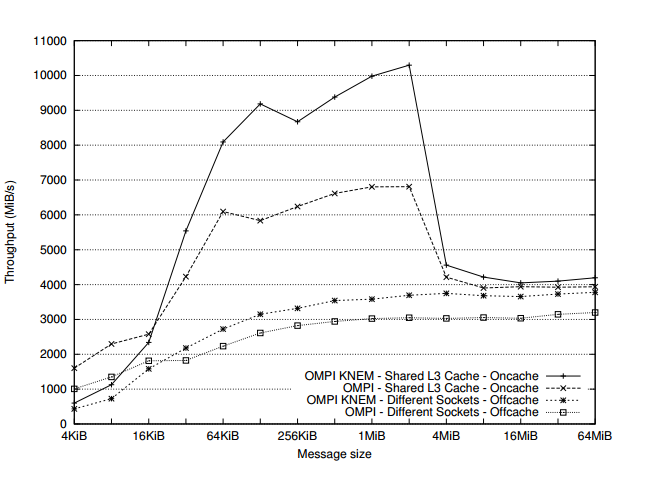
\includegraphics[width=\textwidth]{./images/knem_graph.png}
    \caption{Thoughtput για το IMB PingPong Benchmark}
    \label{fig:Knem}
\end{figure}
\paragraph{}
Στο Σχήμα \ref{fig:Knem} φαίνεται η αύξηση στο ρυθμό ανταλλαγής δεδομένων με χρήση του KNEM για το benchmark IMB PingPong σε ένα NUMA μηχάνημα. Οι περιπτώσεις με όνομα \textit{Shared Cache - Oncache} αφορούν την πιο φιλική προς την cache προσέγγιση, στις οποίες οι διεργασίες που επικοινωνούν μοιράζονται μία μεγάλη cache. Αντίθετα οι περιπτώσεις \textit{Different Sockets - Offcache}, αντιστοιχούν στο χειρότερο σενάριο όπου δεν υπάρχει κοινή cache μεταξύ των διεργασιών.
\paragraph{}
Από το σχήμα φαίνεται ότι στις περιπτώσεις που δεν υπάρχει κοινή cache η επίδοση της επικοινωνίας βελτιώνεται με χρήση του KNEM, καθώς η απώλεια κοινής cache έχει ελάχιστη επίδραση στη Single-Copy διαδικασία που εκτελεί, αντίθετα με την Double-Copy και τους ενδιάμεσους buffers. Όσον αφορά τις περιπτώσεις που υπάρχει κοινή cache, το KNEM υστερεί των υπαρχόντων υλοποιήσεων για μηνύματα με μέγεθος μικρότερα της χωρητικότητας της cache. Κάτι τέτοιο είναι αναμενόμενο καθώς το KNEM εκτελεί κλήσεις συστήματος που εισάγουν σημαντικό overhead στη διαδικασία. Ωστόσο, για μηνύματα με μέγεθος μεγαλύτερο από τη χωρητικότητα της cache το KNEM υπερέχει σημαντικά. Η συνήθης πρακτική είναι η χρήση του KNEM για μεγέθη μηνυμάτων μεγαλύτερα από 4ΚΒ.

\paragraph{}
Εκτός από τη βελτιστοποίηση της point-to-point επικοινωνίας, η επιστημονική κοινότητα ασχολήθηκε και με την collective. Συγκεκριμένα ο S. Li και άλλοι \cite{Sli}, πρότειναν αλγόριθμους για την υλοποίηση συγκεκριμένων collectives (allreduce, reduce, broadcast) σχεδιασμένους ειδικά για αρχιτεκτονική NUMA. Με τη χρήση των αλγορίθμων επιτυγχάνουν κατά μέσο όρο 2.5 φορές καλύτερη επίδοση σε σχέση με τους γενικούς αλγορίθμους που χρησιμοποιούν οι υλοποιήσεις του MPI. Επιπλέον, γίνεται και σύγκριση της επίδοσης με OpenMP με τα αποτελέσματα να υπερέχουν με τη χρήση του MPI και των προσαρμοσμένων αλγορίθμων. 

\section{Κίνητρο}
\paragraph{}
Όπως αναφέραμε πιο πάνω, η εμφάνιση multicore και manycore επεξεργαστών αύξησε το επίπεδο του παραλληλισμού εσωτερικά των κόμβων. Καθώς ο αριθμός των πυρήνων μέσα στους κόμβους συνεχίζει να αυξάνει, η intranode επικοινωνία θα έχει μεγαλύτερο αντίκτυπο στον τελικό χρόνο εκτέλεσης. Συνεπώς, η πρόβλεψη του χρόνου επικοινωνίας σε αρχιτεκτονικές κοινής μνήμης αποκτά όλο και περισσότερη χρησιμότητα.
\begin{figure}[t]
    \centering
    \captionsetup{justification=centering,margin=0cm}
    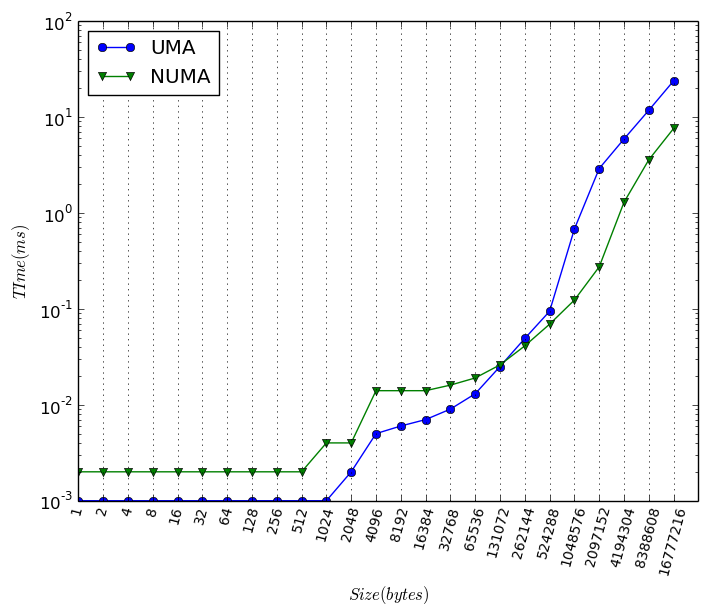
\includegraphics[width=\textwidth]{./images/NUMAvsUMA.png}
    \caption{Συγκριτικό διάγραμμα για τις αρχιτεκτονικές UMA και NUMA για point-to-point επικοινωνία}
    \label{fig:UMAvsNUMA}
\end{figure}
\paragraph{}
Στο Σχημα \ref{fig:UMAvsNUMA} φαίνεται ο χρόνος επικοινωνίας που αναλώνεται για επικοινωνία για ένα απλό benchmark σε αρχιτεκτονικές UMA και NUMA για 8 διεργασίες. Στο benchmark γίνεται ping-pong point-to-point επικοινωνία ανά δύο διεργασίες. Για UMA όλη η επικοινωνία γίνεται μεταξύ σε διεργασίες στον ίδιο επεξεργαστή. Αντίθετα στη NUMA επικοινωνία έχουμε φροντίσει έτσι ώστε όλες οι διεργασίες που επικοινωνούν να βρίσκονται σε διαφορετικά NUMA islands. Σαν αποτέλεσμα, όλη η επικοινωνία περνά πάνω από το δίκτυο διασύνδεσης των νησιών.

\paragraph{}
Για μηνύματα μήκους μικρότερου από 128KiB παρατηρούμε ότι η επικοινωνία σε αρχιτεκτονική UMA υπερτερεί της NUMA, αφού η καθυστέρηση που εισάγει η χρήση του δικτύου διασύνδεσης των νησιών είναι καθοριστική για τον χρόνο επικοινωνίας. Στην αντίθετη περίπτωση, η NUMA αρχιτεκτονική πετυχαίνει μικρότερους χρόνους επικοινωνίας. Καθώς τα μηνύματα μεγαλώνουν, η επικοινωνία σε UMA αρχιτεκτονική περιορίζεται από φαινόμενα της κρυφής μνήμης και τον ανταγωνισμό στο δίαυλο μνήμης ενώ η NUMA αρχιτεκτονική μπορεί να διαχειριστεί τα μεγαλύτερα μηνύματα γρηγορότερα εκμεταλλευόμενη το ψηλό bandwidth του δίκτυου διασύνδεσης. 


\paragraph{}
Αναφορικά με τη collective επικοινωνία, στο Σχήμα \ref{fig:UMAvsNUMA_alltoall} δίνονται οι χρόνοι επικοινωνίας για τις δύο αρχιτεκτονικές και το collective \textit{alltoall}. Σημειώνουμε ότι τα μεγέθη που αναφέρονται στη γραφική δεν αναφέρονται στο μήκος του buffer εισόδου αλλά στο μήκος των μηνυμάτων που καταλήγουν να ανταλλάσσουν οι διεργασίες. Φαίνεται ότι το ίδιο μοτίβο ακολουθεί και η συλλογική επικοινωνία, με τις δύο αρχιτεκτονικές να υπερέχουν για διαφορετικά μεγέθη μηνύματος. 
\begin{figure}[t]
    \centering
    \captionsetup{justification=centering,margin=0cm}
    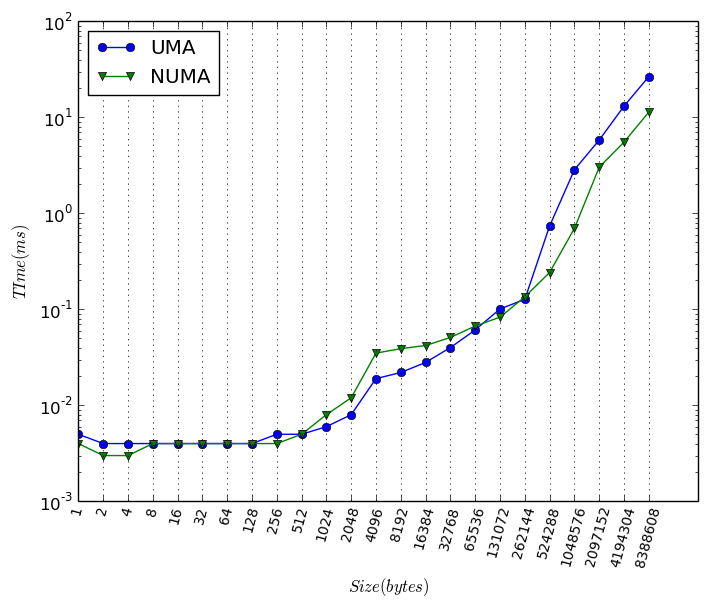
\includegraphics[width=\textwidth]{./images/NUMAvsUMA_alltoall.png}
    \caption{Συγκριτικό διάγραμμα για επικοινωνία σε αρχιτεκτονικές UMA και NUMA για το collective alltoall}
    \label{fig:UMAvsNUMA_alltoall}
\end{figure}
\paragraph{}
 Ακόμη και με μικρό αριθμό διεργασιών, φαίνεται ότι η μοντελοποίηση της επικοινωνίας δεν είναι απλή διαδικασία. Η διάκριση ανάμεσα στους δύο τύπους επικοινωνίας, εσωτερικής του επεξεργαστή και εξωτερικής,  είναι απαραίτητη για να πετύχει κάποιος καλά αποτελέσματα, αφού με βάση την κατανομή των διεργασιών στους πόρους του συστήματος και τα δεδομένα που ανταλλάσσουν, διαφορετικά κομμάτια του συστήματος δέχονται πίεση και άλλα χαρακτηριστικά της αρχιτεκτονικής είναι κυρίαρχα στο χρόνο επικοινωνίας.
\paragraph{}
Έτσι προτείνουμε μία προσέγγιση βασισμένη σε τεχνικές μηχανικής μάθησης, με σκοπό την πρόβλεψη του χρόνου επικοινωνίας MPI εφαρμογών σε αρχιτεκτονική κοινής μνήμης για ασύγχρονη point-to-point αλλά και collective επικοινωνία η οποία διαχωρίζει τις δύο επικοινωνίες.
\paragraph{}
Αποφασίσαμε λοιπόν, να αναλύσουμε την επικοινωνία από τη σκοπιά της MPI εφαρμογής αλλά και τη θέση της στο μηχάνημα. Έτσι ποσοτικοποιούμε τους δύο τύπους επικοινωνίας ξεχωριστά για να μπορούν τα μοντέλα επικοινωνίας που θα αναπτύξουμε να υπολογίζουν την επίδραση της κάθε μίας. Παρόλα αυτά, η μεθοδολογία μας δεν είναι δεσμευτική και θα μπορούσε κάλλιστα να εφαρμοστεί σε δεδομένα εξαγόμενα από το σύστημα εκτέλεσης του MPI. Επιπλέον, η ίδια διαδικασία μπορεί να εφαρμοστεί σε οποιοδήποτε μοντέλο ανταλλαγής μηνυμάτων, χωρίς να είναι απαραίτητη η διάκριση μεταξύ των δύο τύπων επικοινωνίας. Τέλος, πολλά frameworks με σκοπό την ανάλυση μεγάλου όγκου δεδομένων (big data analytics), όπως τα Hama \footnote{http://hama.apache.org} και Pregel \cite{PREGEL}, κάνουν χρήση ενός προγραμματιστικού μοντέλου που ονομάζεται bulk synchonous. Υπολογισμοί και επικοινωνία γίνονται επαναληπτικά σε διακριτές φάσεις με τις διεργασίες να συγχρονίζονται στο τέλος κάθε επανάληψης. Τέτοιου είδους εφαρμογές συνήθως εκτελούνται σε μηχανήματα NUMA μεγάλης κλίμακας, με τη μεθοδολογία μας να είναι ιδανική για πρόβλεψη του χρόνου επικοινωνίας τους. 

\section{Σχετικές Εργασίες}
\paragraph{}
Φυσικά, έχουν προταθεί και άλλες μεθοδολογίες με σκοπό την πρόβλεψη της επίδοσης της επικοινωνίας. Οι περισσότερες ωστόσο, μοντελοποιούν την διαδικασία της επικοινωνίας με χρήση αναλυτικών μοντέλων.
\paragraph{}
Μία πρώτη επιτυχημένη προσπάθεια για πρόβλεψη της point-to-point επικοινωνίας ήταν το μοντέλο του Hockney \cite{HOCKNEY}. Σύμφωνα με το μοντέλο αυτό η καθυστέρηση μπορεί να εκφραστεί σαν:
\begin{align*}
t(s) = t_0 + \frac{s}{b}
\end{align*}
όπου $t$ η καθυστέρηση, $t_0$ η αρχική καθυστέρηση, $s$ το μήκος του μηνύματος και $b$ το μέγιστο εύρος ζώνης (bandwidth) που μπορούμε να πετύχουμε. Ωστόσο, σε σύγχρονες υλοποιήσεις του MPI, το πρωτόκολλο επικοινωνίας αλλάζει ανάλογα με το μήκος του μηνύματος. Κάτι τέτοιο δεν μπορεί να μοντελοποιηθεί από το μοντέλο Hockney καθώς οι παράμετροι του είναι σταθεροί.
\paragraph{}
Μία άλλη προσπάθεια είναι το μοντέλο LogP \cite{LogP}. Πρόκειται για ένα μοντέλο που μπορεί να εφαρμοστεί σε κάθε μηχάνημα και αγνοεί τις λεπτομέρειες της υλοποίησης του πρωτοκόλλου επικοινωνίας. Αποτελείται μόλις από τέσσερις παραμέτρους, την καθυστέρηση (latency - L) ανάμεσα στα modules  για μήνυμα μεγέθους μίας λέξης (συνήθως 8 bytes), το overhead (O), που αφορά το χρόνο που ο επεξεργαστής καταναλώνει για την αποστολή, το κενό (gap - g), που αναπαριστά το ελάχιστο χρονικό διάστημα μεταξύ συνεχόμενων αποστολών μηνυμάτων και τον αριθμό των επεξεργαστών (processors - P). Στις τέσσερις  παραμέτρους που το συνθέτουν οφείλει και το όνομα του. Χρησιμοποιείται κατά κόρο για να δώσει κατευθυντήριες γραμμές  στους σχεδιαστές μηχανημάτων και σαν βάση για γρήγορη ανάπτυξη φορητών παράλληλων αλγορίθμων.

\paragraph{}
Από το 1994, που προτάθηκε το LogP, έχουν αναπτυχθεί πολλές επεκτάσεις του. Οι περισσότερες πρόσθεταν στο μοντέλο νέες παραμέτρους με σκοπό την μοντελοποίηση φαινομένων τα οποία δεν λάμβανε υπόψη.  Το LogGP \cite{LogGP}, προσπαθούσε να συμπεριλάβει τις αλλαγές στο bandwidth για μεγάλα μηνύματα εισάγοντας την παράμετρο G. Επιπλέον της G, το μοντέλο LogGPS  \cite{LogGPS}, έκανε χρήση της παραμέτρου S με σκοπό να συλλάβει αλλαγές στο πρωτόκολλο επικοινωνίας με βάση το μέγεθος του μηνύματος.  

\paragraph{}
Πέραν του LogP και των επεκτάσεων του, που είναι σχεδιασμένα με βάση την τοπολογία της internode επικοινωνίας, μέθοδοι έχουν αναπτυχθεί και για την intranode. Συγκεκριμένα, οι S. Ramos και T. Hoefler \cite{ramos2013modeling}, στην προσπάθεια τους να δώσουν ένα μοντέλο επίδοσης για manycore και multicore αρχιτεκτονικές ανέπτυξαν αναλυτικά μοντέλα για cache-to-cache επικοινωνία. Βασίστηκαν στα πρωτόκολλα που υλοποιούν τη συνοχή της κρυφής μνήμης (cache coherency) τα οποία περιγράφονται με μηχανές πεπερασμένων καταστάσεων. Ανάλογη προσπάθεια, με σκοπό την βελτιστοποίηση της επικοινωνίας έγινε από τον Β. Putigny και άλλους \cite{putigny}. Στόχευαν στη χρήση microbenchmarks με σκοπό την εξαγωγή χαρακτηριστικών της cache καθώς είναι κρίσιμη για την intranode επικοινωνία. Με τα αποτελέσματα μοντελοποίησαν την επικοινωνία πάνω από κοινή μνήμη, επίσης βασιζόμενοι στο πρωτόκολλο συνοχής της κρυφής μνήμης και πρότειναν τεχνικές μέσω των οποίων MPI υλοποιήσεις μπορούν να αυξήσουν την απόδοση της. Τέλος, σε μία πρόσφατη προσπάθεια, αναπτύχθηκε το αναλυτικό μοντέλο \textit{τ-Lop} \cite{tlop}, δίνοντας ένα περίπλοκο μοντέλο επικοινωνίας για collective επικοινωνία χρησιμοποιώντας τους αλγορίθμους που την υλοποιούν, το οποίο παρουσιάζει αξιοσημείωτη ακρίβεια. 

\paragraph{}
Σε γενικές γραμμές, τα αναλυτικά μοντέλα πρέπει να θυσιάσουν την απλότητα τους για να πετύχουν τα αποτελέσματα τους. Καθώς οι αρχιτεκτονικές γίνονται πιο περίπλοκες πρέπει να λαμβάνουν υπόψη τους ακόμα περισσότερα φαινόμενα σε μία ατέλειωτη προσθήκη μεταβλητών. Από την άλλη μεριά, εμπειρικά μοντέλα, που χρησιμοποιούν μετρήσεις από το κάθε μηχάνημα για μοντελοποιήσουν και προβλέψουν την επικοινωνία,  είναι πολύ πιο εύρωστα, παρόλο που απαιτούν εκτέλεση των μετρήσεων σε κάθε μηχάνημα ξεχωριστά. Επιπλέον, αν οι μετρήσεις που περιλαμβάνουν καταφέρνουν να συλλάβουν τα φαινόμενα που διέπουν την επικοινωνία μπορούν να δώσουν πολύ καλά αποτελέσματα με μία σχετικά αυτόματη διαδικασία.
\paragraph{}
Επίσης, σε αναλογία με τα αναλυτικά μοντέλα, μπορούμε να εξετάσουμε και μετρήσεις που αποτυπώνουν τη συμπεριφορά του πρότυπου επικοινωνίας. Αφού πρόκειται για εμπειρικά μοντέλα, θα εντοπίσουν αν κάτι τέτοιο συμβαίνει μέσω των μετρήσεων και θα το μοντελοποιήσουν ανάλογα. 
\paragraph{}
Οι Bhatele και άλλοι \cite{bhatele}, παρουσίασαν πολύ ακριβείς προβλέψεις χρόνου επικοινωνίας, για internode επικοινωνία, κάνοντας χρήση μεθόδων μηχανικής μάθησης. Ωστόσο, η μεθοδολογία τους δεν είναι εφαρμόσιμη για πρόβλεψη πριν την εκτέλεση της εφαρμογής, καθώς χρησιμοποίησαν μετρικές, όπως performance counters, που είναι διαθέσιμες μετά το πέρας της εκτέλεσης της εφαρμογής. Ουσιαστικά σκοπός τους δεν ήταν η πρόβλεψη της επίδοσης της επικοινωνίας, αλλά να προσδιορίσουν τους παράγοντες που επηρεάζουν τη συμφόρηση στα δίκτυα διασύνδεσης.

\section{Περιγραφή Μηχανήματος}
\paragraph{}
Όλα τα πειράματα μας διεξήχθησαν στο μηχάνημα \textit{sandman}. Περιλαμβάνει τέσσερις Intel Xeon E5-4620, τέταρτης γενιάς  συνδεδεμένους  μέσω Intel QuickPath Interconnect. Κάθε ένας από αυτούς αντιστοιχεί σε ένα κόμβο NUMA και διαθέτει 64GiB τοπικής κύριας μνήμης(RAM), με το σύνολο του μηχανήματος να ανέρχεται στα 256GiB. Εντός του κάθε επεξεργαστή υπάρχουν 8 πυρήνες που υποστηρίζουν από δύο νήματα. Κάθε πυρήνας έχει  δύο επίπεδα ιδιωτικής κρυφής μνήμης μεγέθους 32KiB και 256KiB ενώ επιπρόσθετα οι πυρήνες εντός ενός επεξεργαστή μοιράζονται κρυφή μνήμη μεγέθους 16MiB. Μία σχηματική αναπαράσταση του μηχανήματος δίνεται στο Σχημα \ref{fig:sandman}.  
\begin{figure}[ht]
    \centering
    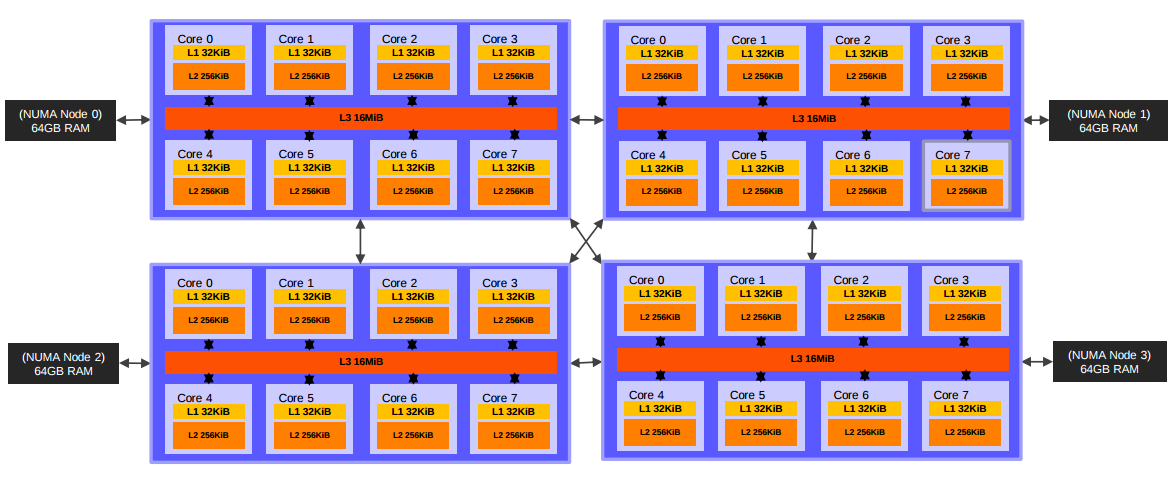
\includegraphics[width=1.1\textwidth]{./images/sandman.png}
    \caption{Αναπαράσταση του μηχανήματος Sandman}
    \label{fig:sandman}
\end{figure}

\chapter{Μοντελοποίηση}
\fancyhead[RE,LO]{Μοντελοποίηση}
\paragraph{}

Σε αυτό το κεφάλαιο καταπιανόμαστε με τα μοντέλα μηχανικής μάθησης που χρησιμοποιήσαμε για την μοντελοποίηση της επικοινωνίας, τις λεπτομέρειες που αφορούν τα εξαγόμενα χαρακτηριστικά από τις εφαρμογές, και τα benchmarks που χρησιμοποιήσαμε με σκοπό την εξαγωγή των σημείων που προορίζονται για την εκπαίδευση των μοντέλων επικοινωνίας.


\section{Μηχανική Μάθηση}
Όπως αναφέραμε πιο πάνω, σκοπός της δουλειάς μας είναι η πρόβλεψη του χρόνου επικοινωνίας μιας εφαρμογής με τεχνικές μηχανικής μάθησης και συγκεκριμένα, επιτηρούμενης μάθησης (supervised learning). Για την εκπαίδευση του μοντέλου, απαιτείται η χρήση κάποιων δειγμάτων, τα οποία σε όρους μηχανικής μάθησης αποτελούν το σύνολο εκπαίδευσης (training set). Κάθε ένα από αυτά τα δείγματα περιέχει ένα διάνυσμα χαρακτηριστικών (feature vector) και τη τιμή της μεταβλητής που το μοντέλο καλείται να προβλέψει. 
\paragraph{}
Η ακρίβεια του μοντέλου στηρίζεται σε πολλές παραμέτρους. Αρχικά, τα χαρακτηριστικά που επιλέγει κανείς πρέπει να αντικατοπτρίζουν τη συμπεριφορά της μεταβλητής. Ωστόσο, υπερβολικός αριθμός χαρακτηριστικών εισάγει μεγάλη πολυπλοκότητα στο μοντέλο, έτσι πρέπει να συμπεριλαμβάνουμε χαρακτηριστικά στο training set με φειδώ. Τέλος, συνίσταται το training set να περιλαμβάνει δείγματα για ένα μεγάλο εύρος των χαρακτηριστικών, σε αναλογία με τις περιπτώσεις που θέλουμε να προβλέψουμε.
\paragraph{}
Στην περίπτωση της εργασίας μας, τα χαρακτηριστικά του training set ήταν μετρικές εξαγόμενες με βάση τις παραμέτρους εκτέλεσης του MPI, την εφαρμογή, και τη θέση των διεργασιών στους πόρους του συστήματος, ενώ η μεταβλητή που το μοντέλο καλείται να προβλέψει είναι ο χρόνος επικοινωνίας. Αφού ο χρόνος παίρνει συνεχείς τιμές το πρόβλημα ανήκει στην κατηγορία της παλινδρόμησης (regression). Τέλος, σημειώνουμε ότι επιλέξαμε χαρακτηριστικά τα οποία μπορούν να εξαχθούν χωρίς την εκτέλεση της εφαρμογής. Σε άλλη περίπτωση η έννοια της πρόβλεψης δεν έχει νόημα. 

\subsection{Μέθοδοι για Regression}
\paragraph{}
Για την επίλυση προβλημάτων regression έχουν προταθεί πολλές μέθοδοι. Παραμετρικά μοντέλα, όπου τα χαρακτηριστικά πολλαπλασιασμένα με βάρη (παραμέτρους) σχηματίζουν μία συνάρτηση, γραμμική ή μη, είναι αρκετά συνήθη. Τέτοια μοντέλα απαιτούν τον ορισμό της μορφής της συνάρτησης από το χρήστη που πρέπει να έχει συναίσθηση του πως τα χαρακτηριστικά επηρεάζουν τη μεταβλητή, με τη μέθοδο να αναλαμβάνει τον υπολογισμό των παραμέτρων ικανοποιώντας κάποιο κριτήριο. Επιπρόσθετα, είναι ευάλωτα στην <<κατάρα της διαστασιμότητας>> με την πολυπλοκότητα του μοντέλου να αυξάνει εκθετικά με τον αριθμό των χαρακτηριστικών. Ωστόσο παρέχουν μία κλειστή συνάρτηση που συνδέει αναλυτικά την μεταβλητή με τα χαρακτηριστικά.
\paragraph{}
Από την άλλη μεριά μη παραμετρικά μοντέλα, όπως δέντρα αποφάσεων και μέθοδοι που συνδυάζουν τα αποτελέσματα τους(ensemble methods) κάνουν τη διαδικασία της εκπαίδευσης πολύ πιο αυτοματοποιημένη. Επιλέγουν ποια χαρακτηριστικά επηρεάζουν τη μεταβλητή περισσότερο, δεν απαιτούν καμιά κανονικοποίηση στις τιμές των χαρακτηριστικών ενώ καμία πληροφορία για το πως τα χαρακτηριστικά συσχετίζονται με τη μεταβλητή δεν πρέπει να δοθεί από το χρήστη. Επιπλέον, αφού τα περισσότερα χρησιμοποιούν δεντρικές δομές, δεν επηρεάζονται αρνητικά αν τα χαρακτηριστικά έχουν μη γραμμική σχέση με τη μεταβλητή.
\subsection{Μέθοδοι Ensemble}
\paragraph{}
Η μέθοδος που χρησιμοποιούμε ανήκει στην κατηγορία ensemble. Η βασική ιδέα είναι η σύνθεση προβλέψεων από απλές μεθόδους regression με σκοπό την αναπαράσταση από το μοντέλο περίπλοκων συναρτήσεων, μείωση της διασποράς των αποτελεσμάτων και περιορισμού της υπερ-προσαρμογής (overfitting) των μοντέλων στο training set. Στις περισσότερες περιπτώσεις, οι αλγόριθμοι βασίζονται σε απλά δέντρα αποφάσεων. Ανάλογα με τον τρόπο που συνθέτουν τα αποτελέσματά τους, οι αλγόριθμοι χωρίζονται σε δύο κατηγορίες: τις Bagging Μεθόδους, όπως τα  random forest και τα extremely randomized trees που προβλέπουν τη μεταβλητή με βάση το μέσο όρο των προβλέψεων των επιμέρους δέντρων και τις Boosting Μεθόδους, όπως την AdaBoost και την Gradient Boosting Regressor Tree όπου σε κάθε βήμα δημιουργούν νέους εκτιμητές που δίνουν έμφαση στα σημεία που τα προηγούμενα μοντέλα δεν υπολόγιζαν με αρκετή ακρίβεια. 

\subsection{Αλγόριθμος Gradient Boosting Regression Tree}
\paragraph{}
Στα πειράματα μας κάναμε εκτεταμένη χρήση του αλγορίθμου \textit{Gradient Boosting Regression Tree} (GBRT \cite{GBRT}), η υλοποίηση του οποίου παρέχεται στο \textit{scikit-learn} της \textit{Python} \cite{scikit}. Καθώς πρόκειται για Boosting μέθοδο, σε κάθε επανάληψη δημιουργείται ένας νέος εκτιμητής ο οποίος προσαρμόζεται στο ήδη υπάρχων μοντέλο με βάση την αρνητική βαθμίδα (gradient) μίας συνάρτησης υπολογισμού του σφάλματος. 
\paragraph{}
O GBRT μας δίνει τη δυνατότητα να ρυθμίσουμε αρκετές παραμέτρους με σκοπό την επίτευξη καλύτερων αποτελεσμάτων ανάλογα με τις ιδιαιτερότητες των δειγμάτων. Για την επίτευξή καλύτερων προβλέψεων εξετάσαμε σωρεία παραμέτρων. Συγκεκριμένα, οι παράμετροι που μας απασχόλησαν ήταν:
\begin{itemize}
\item[] \textbf{n\_estimator:} Ο αριθμός των δέντρων απόφασης που θα ενταχθούν επαναληπτικά στο τελικό δέντρο. Ταυτίζεται με τον αριθμό των επαναλήψεων.
\item[] \textbf{learning\_rate:} Ο ρυθμός μάθησης. Αφορά τον αντίκτυπο που έχει ένα νέο δέντρο στο ήδη υπάρχων.

\item[] \textbf{min\_samples\_split:} Ο ελάχιστος αριθμός δειγμάτων για να σπάσει ένας υπάρχων κόμβος σε δύο.

\item[] \textbf{min\_samples\_leaf:} Ο ελάχιστος αριθμός δειγμάτων για να θεωρηθεί ένας κόμβος, φύλλο.

\item[] \textbf{max\_depth:} Το μέγιστο βάθος που μπορεί να φτάσει το δέντρο.

\item[] \textbf{loss:} Η συνάρτηση υπολογισμού του σφάλματος. Δίνεται δυνατότητα επιλογής από μερικές προκαθορισμένες. 
\end{itemize}

\paragraph{}
Ωστόσο, οι μη παραμετρικές μέθοδοι, συμπεριλαμβανομένου και του αλγορίθμου GBRT, δεν μας παρέχουν με μία κλειστή αναλυτική μορφή για το πως προκύπτει ο χρόνος επικοινωνία. Παρόλα αυτά, με τη βοήθεια του scikit-learn, μπορέσαμε να εξάγουμε μία διαβάθμιση για τα χαρακτηριστικά με σκοπό να βγάλουμε συμπεράσματα σχετικά με το ποια επηρεάζουν περισσότερο το χρόνο επικοινωνίας. Η διαβάθμιση αυτή δεν είναι τελείως αντιπροσωπευτική αναφορικά με τα χαρακτηριστικά που επηρεάζουν την τελική πρόβλεψη. Για παράδειγμα, αν κάποιο χαρακτηριστικό βρίσκεται στα ψηλότερα επίπεδα του δέντρου απόφασης θα έχει αναπόφευκτα ψηλή θέση στη διαβάθμιση αλλά να απαιτείται και η συνδρομή άλλων χαρακτηριστικών στα χαμηλότερα επίπεδα για ακριβή πρόβλεψη.

\subsection{Επιλογή Χαρακτηριστικών}
\paragraph{}
Καθώς τα training set που εξετάζουμε περιέχουν σωρεία χαρακτηριστικών, σε μερικές περιπτώσεις κρίθηκε αναγκαία η χρήση μεθόδων επιλογής χαρακτηριστικών (feature selection) με σκοπό την απόρριψη μετρικών που δεν επηρεάζουν σημαντικά το χρόνο επικοινωνίας. Η μέθοδος που χρησιμοποιήσαμε στα πειράματα μας ήταν επιλογή χαρακτηριστικών μέσω της regression μεθόδου \textit{Support Vector Regressor (SVR)}. Συγκεκριμένα εκπαιδεύαμε ένα SVR μοντέλο με όλα τα δείγματα εκπαίδευσης. Μετέπειτα, με βάση τη διαβάθμιση της σημασίας(importance) που είχαμε στη διάθεση μας, αφαιρούσαμε από το αρχικό training set τα χαρακτηριστικά που είχαν μικρότερο importance από τον μέσο όρο των importances για όλα τα χαρακτηριστικά.

\subsection{Μέθοδοι εξαγωγής Communication Patterns}
\paragraph{}
Είχαμε στη διάθεσή μας αρκετές μεθόδους για την εξαγωγή των communication patterns. Η πιο εύκολη και ευθύγραμμη ήταν η προσθήκη συναρτήσεων στις εφαρμογές οι οποίες επιστρέφουν το communication pattern τους. Ωστόσο, αφού για τη ανάκτηση του communication pattern έπρεπε να έχει τελειώσει η εκτέλεση της εφαρμογής, δεν ήταν κατάλληλη για πρόβλεψη. Μία ανάλογη πρακτική, ήταν η επέκταση των εντολών αποστολής του \textit{OpenMPI} έτσι ώστε με κάθε κλήση των συναρτήσεων αποστολής μηνυμάτων να τυπώνουν τα αναγνωριστικά των διεργασιών που εμπλέκονται στην αποστολή και το μέγεθος των δεδομένων που αποστέλλονται. Η μεθοδολογία αυτή, πέραν του ότι είναι αρκετά περίπλοκη, εμφανίζει το ίδιο μειονέκτημα με την προηγούμενη και επίσης εγκαταλείφθηκε.

\paragraph{}
Τελικά, για κάθε εφαρμογή που μας απασχόλησε, είτε για σκοπούς benchmarking είτε για αξιολόγηση των μοντέλων επικοινωνίας, αναπτύξαμε σειριακές εκδόσεις που υπολόγιζαν το communication pattern τους. Τα ορίσματα τους περιελάμβαναν κάποιες από τις παραμέτρους εκτέλεσης των εφαρμογών, όπως τον αριθμό των MPI διεργασιών που έχουν άμεση επίδραση στις ανταλλαγές δεδομένων που λαμβάνουν χώρα, αλλά και ορίσματα συγκεκριμένα για κάθε εφαρμογή. Οι εκδόσεις αυτές δεν εκτελούσαν ούτε το υπολογιστικό κομμάτι, ούτε την επικοινωνία μεταξύ των διεργασιών. Έτσι δεν προσθέτουν πολυπλοκότητα στο κρίσιμο μονοπάτι της μεθοδολογίας μας. Τέλος, είναι ανεξάρτητες από το μηχάνημα και τη θέση των διεργασιών σε αυτό.

\paragraph{}
Το πιο σημαντικό πλεονέκτημα των σειριακών εκδόσεων, ήταν η δυνατότητα εξαγωγής των communication patterns πριν την εκτέλεση της εφαρμογής. Σαν αποτέλεσμα, σε κάποιο ρεαλιστικό σενάριο βελτιστοποίησης, μπορούμε να χρησιμοποιήσουμε τα μοντέλα μας για να πάρουμε τις προβλέψεις πριν την εκτέλεση της εφαρμογής, και με βάση τα αποτελέσματα να επιλέξουμε το configuration που μας παρέχει τα περισσότερα πλεονεκτήματα σχετικά με το μέγεθος των πόρων που θα χρησιμοποιήσουμε και το χρόνο επικοινωνίας που απαιτείται.

\section{Εξαγόμενες Μετρικές}
\paragraph{}
Κρίσιμο κομμάτι στη μεθοδολογία μας ήταν η εξαγωγή των χαρακτηριστικών από τις εφαρμογές. Σαν χαρακτηριστικά, εξάγαμε μετρικές με βάση τον αριθμό των ζητούμενων πόρων, το μοτίβο επικοινωνίας της κάθε εφαρμογής και τη θέση των διεργασιών στο μηχάνημα. 

\paragraph{}
Παρόλο που υπάρχουν κοινές μετρικές για Non-Blocking point-to-point και collective επικοινωνία πολλές διαφέρουν όπως και η διαδικασία για την εξαγωγή τους. Στις δύο επόμενες υποενότητες παραθέτουμε αναλυτικά τη διαδικασία που ακολουθήσαμε για τους δύο τύπους επικοινωνίας ξεχωριστά.
\subsection{Εξαγωγή Μετρικών Non-Blocking Επικοινωνίας}
\paragraph{}
Όσο αφορά τις μετρικές για την Non-Blocking point-to-point επικοινωνία, με βάση τα δεδομένα που απαιτούν για την εξαγωγή τους, τις χωρίσαμε σε τρεις κατηγορίες. Ο πρώτος τύπος μετρικών ήταν οι παράμετροι που δίνονται στο σύστημα εκτέλεσης του MPI πριν την εκτέλεση της εφαρμογής από το χρήστη. Η πληροφορία είναι απαραίτητη στη μεθοδολογία μας καθώς αποτελεί βάση για τις επόμενες μετρικές που εξάγαμε.
\paragraph{}
Ο δεύτερος τύπος, ήταν μετρικές εξαγόμενες από το προφίλ επικοινωνίας (com\-munication pattern) της κάθε εφαρμογής. Βασιζόμενοι σε αυτό υπολογίσαμε μετρικές στο επίπεδο της MPI διεργασίες. Οι μετρικές αυτές είναι ανεξάρτητες από το mapping των διεργασιών στους διαθέσιμους πόρους. Περιέχουν πληροφορίες για επικοινωνία που λαμβάνει χώρα από τη σκοπιά της διεργασίας-αποστολέας, αγνοώντας την απόσταση της από τη διεργάσία-παραλήπτης.
\paragraph{}
Παρόλα τα πλεονεκτήματα τους, οι προηγούμενες μετρικές αποτυγχάνουν να αποτυπώσουν τη διαφορά ανάμεσα στην επικοινωνία που λαμβάνει χώρα πάνω από το δίκτυο διασύνδεσης των NUMA κόμβων και την επικοινωνία εσωτερικά του κόμβου\footnote{Στα επόμενα βήματα θα αναφερόμαστε στην επικοινωνία μεταξύ των NUMA κόμβων σαν internode και στην επικοινωνία εσωτερικά των κόμβων σαν intranode, αφού στην κλίμακα των μηχανημάτων που μας αφορούν οι κόμβοι είναι τα NUMA islands.}. Σαν αποτέλεσμα, για επόμενο τύπο μετρικών επιλέξαμε μετρικές που βασίζονται στην κατανομή των διεργασιών στους πόρους του συστήματος και στο communication pattern της εφαρμογής. Έτσι εξάγαμε μετρικές στο επίπεδο του κόμβου πετυχαίνοντας το στόχο μας, για διάκριση της επικοινωνίας σε intranode και internode. 

\paragraph{}
Είναι σημαντικό να αναφέρουμε ότι, για να εφαρμόσουμε τη μεθοδολογία μας, ήταν απαραίτητη η γνώση της απεικόνισης των MPI διεργασιών στους πόρους του μηχανήματος. Έτσι σε όλα τα πειράματα μας η θέση των διεργασιών στους πόρους δινόταν ρητώς στο σύστημα εκτέλεσης του MPI. Ισοδύναμα, αν το περιβάλλον εκτέλεσης ανάθετε τις διεργασίες στους πόρους με συγκεκριμένη πολιτική (blocked,round-robin etc), μπορούσαμε να υπολογίσουμε ευθύγραμμα την απεικόνιση πριν την εκτέλεση της εφαρμογής. Η ρητή επιλογή της απεικόνισης κρίθηκε πιο βολική, αφού μας έδινε τη δυνατότητα να πάρουμε δείγματα εκπαίδευσης για σωρεία διαφορετικών mappings που είναι άμεσα συσχετισμένα με τον τρίτο τύπο μετρικών. Παρόλα αυτά, δεν πρόκειται για δεσμευτική επιλογή. Η μοναδική προϋπόθεση είναι η γνώση της απεικόνισης πριν τη εκτέλεση της εφαρμογής.
\paragraph{}
Επιπλέον, όλες οι μετρικές είναι υπολογισμένες με βάση τα δεδομένα που αποστέλλονται αγνοώντας αν κάποια διεργασία λαμβάνει πολύ περισσότερα δεδομένα από ότι αποστέλλει με ότι αυτό συνεπάγεται για την επικοινωνία. Εντούτοις, σε περιπτώσεις στις οποίες διεργασίες αποστέλλουν πολλά δεδομένα χωρίς να λαμβάνουν ανάλογο αριθμό, κοινή πρακτική είναι η χρήση άλλων μεθόδων αποστολής δεδομένων και όχι point-to-point επικοινωνίας.  

\paragraph{}
Παρακάτω θα αναφερθούμε αναλυτικά σε όλες τις μετρικές που εξάγαμε για κάθε τύπο.
\paragraph{Μετρικές με βάση τις παραμέτρους εκτέλεσης του MPI}
\begin{itemize}
\item \textbf{Κόμβοι} \textit{(Νodes-N)} : Ο αριθμός των κόμβων στους οποίους εκτελείται η εφαρμογή. 
\item \textbf{Διεργασίες ανά Κόμβο} \textit{(ProcessesPerNode-PPN)} : Ο αριθμός των MPI διεργασιών ανά κόμβο. Επηρεάζει τον όγκο της επικοινωνίας εσωτερικά του κόμβου, ανάλογα με το communication pattern της εφαρμογής.
\item \textbf{Σύνολο MPI διεργασιών} \textit{(Processes-P)} : Ο συνολικός αριθμός των MPI διεργασιών που ζητά ο χρήστης.
\end{itemize}

\paragraph{Μετρικές με βάση το μοτίβο επικοινωνίας της εφαρμογής\\} 
Οι μετρικές αυτές είναι υπολογισμένες ανά διεργασία. Στο τελικό training set περιέχεται η ελάχιστη, μέση και μέγιστη τιμή τους. 
\begin{itemize}
\item \textbf{Μέγεθος Μηνυμάτων ανά διεργασία} \textit{(Size-S)} :  Το μέγεθος των μηνυμάτων που αποστέλλονται από τις διεργασίες. Για μεγάλα μηνύματα το πρωτόκολλο επικοινωνίας μπορεί να αλλάξει.
\item \textbf{Αριθμός Μηνυμάτων ανά διεργασία} \textit{(Messages-M)} : Το άθροισμα των μηνυμάτων που αποστέλλονται από κάθε διεργασία. Ανάλογα με τον αριθμό των μηνυμάτων, μηνύματα ίσως σειριοποιούνται ή  συνενώνονται. 
\item \textbf{Όγκος Δεδομένων ανά διεργασία} \textit{ (ProcessTraffic-PT) } : Το άθροισμα των μηνυμάτων που αποστέλνονται ανά διεργασία. Ο όγκος των δεδομένων ανά διεργασία μπορεί να εντοπίσει φαινόμενα συμφόρησης. 
\end{itemize}

\paragraph{Μετρικές με βάση την κατανομή των διεργασιών στο μηχάνημα και το μοτίβο επικοινωνίας\\}
Για όσες μετρικές από αυτές είναι υπολογισμένες ανά κόμβο, στο training set περιλαμβάνεται η ελάχιστη, μέση και μέγιστη τιμή τους.
\begin{itemize}
\item \textbf{Εσωτερικός Όγκος Δεδομένων ανά κόμβο} \textit{(IntraΝodeΤraffic-NT)} : Αφορά τον όγκο των δεδομένων που ανταλλάσσουν διεργασίες που βρίσκονται στον ίδιο κόμβο. Μπορεί να αντικατοπτρίσει περιπτώσεις συμφόρησης στο διάδρομο δεδομένων εντός του κόμβου. 
\item \textbf{Εσωτερικός Αριθμός Μηνυμάτων ανά κόμβο} \textit{(IntraΝodeΙnjection-NI)} : Ο αριθμός των μηνυμάτων ανάμεσα σε διεργασίες που βρίσκονται στον ίδιο κόμβο.
\item \textbf{Συνολικός Όγκος Δεδομένων εσωτερικά των κόμβων} \textit{(Int\-raVolume-V)} : Όλος ο όγκος των δεδομένων ανάμεσα σε διεργασίες που βρίσκονται στον ίδιο κόμβο. Πρόκειται ουσιαστικά για το άθροισμα όλων των \textit{IntraNodeTraffics}.
\item \textbf{Συνολικός αριθμός μηνυμάτων εσωτερικά των κόμβων} \textit{(Int\-raInjection-VI)} : Το πλήθος όλων των μηνυμάτων που αποστέλλονται εσωτερικά των κόμβων. 
\item \textbf{Εξωτερικός Όγκος Δεδομένων ανά κόμβο} \textit{(InterNodeTraffic-INT)} : Ο όγκος των δεδομένων ανάμεσα σε διεργασίες που βρίσκονται σε διαφορετικούς κόμβους. Μπορεί να αντικατοπτρίσει περιπτώσεις συμφόρησης στο δίκτυο διασύνδεσης των νησιών NUMA. 
\item \textbf{Εξωτερικός Αριθμός Μηνυμάτων ανά κόμβο} \textit{(InterΝodeΙnjection-INI)} : Ο αριθμός των μηνυμάτων που αποστέλλονται σε διεργασίες που βρίσκονται σε άλλο κόμβο.
\item \textbf{Συνολικός Όγκος Δεδομένων εξωτερικά των κόμβων} \textit{(Int\-erVolume-IV)} : Όλος ο όγκος των δεδομένων ανάμεσα σε διεργασίες που βρίσκονται σε διαφορετικούς κόμβους. Πρόκειται ουσιαστικά για το άθροισμα όλων των \textit{InterNodeTraffics}.
\item \textbf{Συνολικός αριθμός μηνυμάτων εξωτερικά των κόμβων} \textit{(Int\-erInjection-IVI)} : Το πλήθος όλων των μηνυμάτων ανάμεσα σε διεργασίες που βρίσκονται σε διαφορετικούς κόμβους. 
\end{itemize}

\subsection{Εξαγωγή Μετρικών Collective Επικοινωνίας}
\paragraph{}
Η επιλογή και η εξαγωγή των μετρικών για την Collective επικοινωνία ήταν πολύ πιο περίπλοκη διαδικασία σε σχέση με την point-to-point. Οι αλγόριθμοι που χρησιμοποιούνται διαφέρουν από υλοποίηση σε υλοποίηση και αλλάζουν συνεχώς. Συνήθως, τα collectives $scatter,gather$ και $reduce$ βασίζονται σε point-to-point υλοποιήσεις, το $broadcast$ σε ένα δεντρικό αλγόριθμο και τα $allreduce,allgather$ και $alltoall$ σε συνδυασμό των παραπάνω. Η μεγαλύτερη πρόκληση ήταν να κρατήσουμε τη μεθοδολογία μας ανεξάρτητη της υλοποίησης του κάθε collective. Επομένως, θα ήταν πολύ πιο φορητή και θα μπορούσε να εφαρμοστεί και σε άλλες υλοποιήσεις των collectives. Αυτό σήμαινε ότι δεν θα είχαμε στη διάθεση μας το ακριβές communication pattern για κάθε εφαρμογή. Έτσι, για την μοντελοποίηση της επικοινωνίας στηριχτήκαμε σε ένα αφηρημένο communication pattern που φτιάξαμε, ανάλογα με τον κάθε τύπο collective.
\paragraph{}
Θα προσπαθήσουμε να εξηγήσουμε τη λογική μας μέσω ενός παραδείγματος. Ας πάρουμε για παράδειγμα το communication pattern που δίνει η μοντελοποίηση για το collective allgather. Tο συγκεκριμένο collective μαζεύει δεδομένα από όλες τις διεργασίες και τα επιστρέφει σε όλες. Έστω ότι έχουμε ένα allgather με buffer εισόδου μεγέθους $S$ bytes και $N$ MPI διεργασίες. Υποθέτουμε ότι όλοι οι buffers πρέπει να μαζευτούν σε κάποια διεργασία και μετέπειτα να αποσταλούν στις υπόλοιπες. Έτσι όλες οι διεργασίες αποστέλλουν ένα μήνυμα μεγέθους $S$ σε κάποια διεργασία "ρίζα",  η οποία με τη σειρά της αποστέλλει μηνύματα μεγέθους $N\times S$ σε όλες τις άλλες. Θα συμβολίζουμε αυτό το communication pattern με $N - 1 - N$, αφού σε πρώτο στάδιο $N$ διεργασίες αποστέλλουν δεδομένα σε 1 και σε επόμενο, 1 σε $N$. Ωστόσο αυτός ο συμβολισμός δεν περιέχει όλη την πληροφορία του communication pattern αφού δεν περιλαμβάνει το μέγεθος των μηνυμάτων. Για είμαστε πλήρης, θα χρησιμοποιήσουμε και ένα δεύτερο συμβολισμό, που θα περιέχει το μέγεθος των μηνυμάτων που ανταλλάσσονται σε κάθε στάδιο. Έτσι, για το allgather έχουμε το συμβολισμό $S-(N\times S)$ αφού μηνύματα $S$ μεγέθους αποστέλλονται στο πρώτο στάδιο και μηνύματα $N\times S$ στο δεύτερο. Στον Πίνακα \ref{table:coll} φαίνεται πώς μοντελοποιήσαμε κάθε collective που μας απασχόλησε.
\begin{table}[t]
\centering
\caption{Communication Pattern για κάθε collective}
\label{table:coll}
\begin{tabular}{l|c|c}
\textbf{Collective} & \textbf{Μηνύματα} & \textbf{Μέγεθος Μηνυμάτων} \\ \hline
scatter    & 1-N      & S                 \\
gather     & N-1      & S                 \\
reduce     & N-1      & S                 \\
broadcast  & 1-N      & S                 \\
allreduce  & N-1-N    & S-S               \\
allgather  & N-1-N    & S-(N$\times$S)           \\
alltoall   & N-N      & S                
\end{tabular}
\end{table}

\paragraph{}
Αφού πλέον είχαμε στη διάθεση μας τα communication patterns, 	μπορούσαμε να προχωρήσουμε στην επιλογή των μετρικών. Αναλογικά με την point-to-point επικοινωνία χωρίζουμε τις μετρικές σε τρεις κατηγορίες: την πρώτη, που ήταν η ίδια με την point-to-point επικοινωνία και αφορούσε τις παραμέτρους που δίνονται στο σύστημα εκτέλεσης του MPI, τη δεύτερη που περιείχε τις μετρικές που εξάγονται από το communication pattern και την τρίτη με τις μετρικές βασίζονταν στο communication pattern και στο mapping των διεργασιών στο μηχάνημα. 

\paragraph{}
Σε αντίθεση με τις μετρικές της point-to-point επικοινωνίας, στις μετρικές της collective επικοινωνίας έχουμε μετρικές που αφορούν τα δεδομένα που αποστέλλονται αλλά και τα δεδομένα που λαμβάνονται καθώς η επικοινωνία δεν είναι συμμετρική. Παρακάτω παραθέτουμε τις μετρικές για κάθε τύπο αναλυτικά. 
\paragraph{Μετρικές με βάση τις παραμέτρους εκτέλεσης του MPI}
\begin{itemize}
\item \textbf{Κόμβοι} \textit{(Νodes-N)} : Ο αριθμός των κόμβων στους οποίους εκτελείται η εφαρμογή. 
\item \textbf{Διεργασίες ανά Κόμβο} \textit{(ProcessesPerNode-PPN)} : Ο αριθμός των MPI διεργασιών ανά κόμβο. Επηρεάζει τον όγκο της επικοινωνίας εσωτερικά του κόμβου, ανάλογα με το communication pattern της εφαρμογής.
\item \textbf{Σύνολο MPI διεργασιών} \textit{(Processes-P)} : Ο συνολικός αριθμός των MPI διεργασιών.
\end{itemize}

\paragraph{Μετρικές με βάση το μοτίβο επικοινωνίας της εφαρμογής\\} 
Οι μετρικές αυτές είναι υπολογισμένες ανά διεργασία. Στο τελικό training set περιέχεται η ελάχιστη, μέση και μέγιστη τιμή τους. 
\begin{itemize}
\item \textbf{Μέγεθος Μηνυμάτων ανά διεργασία} \textit{(Size-S)} :  Το μήκος των μηνυμάτων που αποστέλλονται από τις διεργασίες.
\item \textbf{Πλήθος Μηνυμάτων ανά διεργασία} \textit{(Messages-M)} : Το πλήθος των μηνυμάτων που αποστέλλονται από κάθε διεργασία.
\item \textbf{Εισερχόμενος Όγκος Δεδομένων ανά διεργασία} \textit{ (IncomingProcess\-Traffic-IPT) } : Το άθροισμα των μεγεθών των  μηνυμάτων που λαμβάνονται ανά διεργασία. 
\item \textbf{Εξερχόμενος Όγκος Δεδομένων ανά διεργασία} \textit{ (OutgoingProcess\-Traffic-ΟPT) } : Το άθροισμα των μεγεθών μηνυμάτων που αποστέλλονται ανά διεργασία.
\end{itemize}

\paragraph{Μετρικές με βάση την κατανομή των διεργασιών στο μηχάνημα και το μοτίβο επικοινωνίας\\}
Για όσες μετρικές από αυτές είναι υπολογισμένες ανά κόμβο, στο training set περιλαμβάνεται η ελάχιστη, μέση και μέγιστη τιμή τους.
\begin{itemize}
\item \textbf{Εσωτερικός Όγκος Δεδομένων ανά κόμβο} \textit{(Intra\-ΝodeΤraffic-NT)} : Αφορά τον όγκο των δεδομένων που ανταλλάσσουν διεργασίες που βρίσκονται στον ίδιο κόμβο. 
\item \textbf{Εσωτερικός Αριθμός Μηνυμάτων ανά κόμβο} \textit{(Intra\-ΝodeΙnjection-NI)} : Ο αριθμός των μηνυμάτων ανάμεσα σε διεργασίες που βρίσκονται στον ίδιο κόμβο.
\item \textbf{Συνολικός Όγκος Δεδομένων εσωτερικά των κόμβων} \textit{(Intra\-Volume-V)} : Όλος ο όγκος των δεδομένων ανάμεσα σε διεργασίες που βρίσκονται στον ίδιο κόμβο. 
\item \textbf{Συνολικός αριθμός μηνυμάτων εσωτερικά των κόμβων} \textit{(Intra\-Injection-VI)} : Το άθροισμα όλων των μηνυμάτων εσωτερικά των κόμβων. 
\item \textbf{Εξωτερικός Όγκος Εξερχόμενων Δεδομένων ανά κόμβο} \textit{(Inter\-NodeOutgoingTraffic-INOT)} : Ο όγκος των εξερχόμενων δεδομένων με προορισμό διεργασίες σε άλλο κόμβο. 
\item \textbf{Εξωτερικός Όγκος Εισερχόμενων Δεδομένων ανά κόμβο} \textit{(Inter\-NodeIncomingTraffic-INIT)} : Ο όγκος των εισερχόμενων δεδομένων με πηγή διεργασίες σε άλλο κόμβο.
\item \textbf{Εξωτερικός Αριθμός Εξερχόμενων Μηνυμάτων  ανά κόμβο} \textit{(Inter\-ΝodeOutgoingΙnjection-INOI)} : Το πλήθος των εξερχόμενων μηνυμάτων με προορισμό διεργασίες που βρίσκονται σε διαφορετικό κόμβο.
\item \textbf{Εξωτερικός Αριθμός Εισερχόμενων Μηνυμάτων  ανά κόμβο} \textit{(Inter\-ΝodeOutgoingΙnjection-INΙI)} : Το πλήθος των εισερχόμενων μηνυμάτων με πηγή διεργασίες σε άλλο κόμβο.
\item \textbf{Συνολικός Όγκος Εξερχόμενων Δεδομένων εξωτερικά των κόμβων} \textit{(Int\-erOutgoingVolume-IVO))} : Όλος ο όγκος των δεδομένων που αποστέλλονται προς διεργασίες που βρίσκονται σε διαφορετικούς κόμβους. 
\item \textbf{Συνολικός Αριθμός  Εξερχόμενων Μηνυμάτων εξωτερικά των κόμβων} \textit{(Int\-erInjection-IVOI)} : Το άθροισμα όλων των μηνυμάτων που αποστέλλονται με αποδέκτη εξωτερικά του κόμβου.
\item \textbf{Συνολικός Όγκος Δεδομένων εξωτερικά των κόμβων} \textit{(Int\-erVolume-IVI)} : Όλος ο όγκος των δεδομένων ανάμεσα σε διεργασίες που βρίσκονται σε διαφορετικούς κόμβους. Πρόκειται ουσιαστικά για το άθροισμα όλων των \textit{InterNodeTraffics}.
\item \textbf{Συνολικός αριθμός μηνυμάτων εξωτερικά των κόμβων} \textit{(Int\-erInjection-IVII)} : Το πλήθος όλων των μηνυμάτων εξωτερικά των κόμβων. 
\end{itemize}
\paragraph{}
\section{Benchmarking}
Όπως αναφέραμε πιο πάνω, αναπόσπαστο κομμάτι της μεθοδολογίας μας είναι η εξαγωγή δεδομένων μέσω benchmarks, τα οποία  χρησιμοποιήσουμε για την εκπαίδευση των μοντέλων επικοινωνίας. Επιλέξαμε benchmarks των οποίων η φάση επικοινωνίας θυμίζει επικοινωνία εφαρμογών, ενώ ταυτόχρονα μας δίνουν τη δυνατότητα ορισμού διαφόρων παραμέτρων με σκοπό την εξαγωγή ενός ευρύ χώρου μετρικών.

\subsection{p2p\_SRR}
\paragraph{}
Αρχικά θα αναφερθούμε στο benchmark p2p\_SRR (point-to-point symmetric with random ratio). Πρόκειται για ένα benchmark βασισμένο στο WICON benchmark \cite{WICON}, όπου τυχαία ζευγάρια κόμβων, με μία διεργασία να τρέχει στον καθένα, ανταλλάσσουν δεδομένα ταυτόχρονα σε μία ping-pong διαδικασία. Ωστόσο, στο p2p\_SRR μας δίνεται η δυνατότητα να τοποθετήσουμε περισσότερες από μία διεργασίες στον κάθε κόμβο. Επιπλέον, για να συμπεριλάβει στους χρόνους την επιρροή πολλών μηνυμάτων, κάθε διεργασία επικοινωνεί με τυχαίες M διεργασίες. Έτσι, καταλήγουμε σε ένα communication pattern στο οποίο κάθε διεργασία στέλνει M μηνύματα σε Μ τυχαίες διεργασίες και αντίστοιχα λαμβάνει απάντηση. Αυτό, σε NUMA αρχιτεκτονική οδηγεί σε ένα communication pattern όπου η αναλογία της internode και intranode επικοινωνίας είναι τυχαία.

\paragraph{}
Κάθε ανταλλαγή μηνυμάτων εκτελείται μερικές εκατοντάδες φορές και κάθε διεργασία μετρά τον τοπικό χρόνο που δαπάνησε για κάθε επανάληψη. Οφείλουμε να αναφέρουμε ότι, πριν την έναρξη κάθε επανάληψης οι διεργασίες συγχρονίζονται για να αποφύγουμε τη μέτρηση χρόνου αναμονής σαν χρόνο επικοινωνίας.  Αφού κάθε διεργασία ταξινομήσει τους χρόνους, ορίζει σαν τοπικό χρόνο επικοινωνίας  κάποιο ποσοστημόριο (quantile) των επαναλήψεων δικής μας επιλογής. Μετέπειτα, μέσω του collective reduce, η εφαρμογή επιστρέφει το μέγιστο χρόνο ανάμεσα από τους τοπικούς. Με αυτή τη τιμή εκπαιδεύσαμε και τα μοντέλα επικοινωνίας στα επόμενα στάδια. Παρόλο που είχαμε την ευχέρεια να επιλέξουμε οποιοδήποτε quantile επιλέξαμε το τρίτο  για να αντισταθμίσουμε αύξηση στο χρόνο επικοινωνίας από φαινόμενα που αγνοούσαμε (cache effects, os noise κ.α.). 
\paragraph{}
Επιπλέον, το benchmark, μας επέτρεπε να ορίσουμε δύο παραμέτρους: τον αριθμό των μηνυμάτων(\textit{M}), μέσω μίας παραμέτρου εισόδου και το μέγεθος του μηνύματος. με μικρές αλλαγές στον πηγαίο κώδικα. Ακόμη, μπορούσαμε να ελέγξουμε τον αριθμό των διεργασιών ανά κόμβο(\textit{PPN}) και τον αριθμό των κόμβων(\textit{N}) μέσω του συστήματος εκτέλεσης του MPI. Τελικά, είχαμε την ευχέρεια να διατρέξουμε τέσσερις παραμέτρους που είχαν άμεση εξάρτηση με όλες τις μετρικές, με αποτέλεσμα ένα training set μεγάλου μεγέθους και αρκετά διαφοροποιημένων σημείων. Το εύρος της κάθε παραμέτρου δίνεται στον Πίνακα \ref{table:NBp2p}.

\begin{table}[h]
\centering
\footnotesize
\caption{Ο χώρος παραμέτρων για το benchmark \textit{p2p\_SRR}}
\label{table:NBp2p}
\begin{tabular}{c|cc}
\multirow{2}{*}{Παράμετρος} & \multicolumn{2}{c}{Αρχιτεκτονική} \\ 
                            & UMA             & NUMA            \\ \hline \hline
N                           & 1               & 2-4             \\
PPN                         & 2-8             & 1-8             \\
Size                        & 1B-16MiB        & 1B-16MiB        \\
Messages                    & 1-8             & 1-8             \\ \hline
\#samples                   & 800             & 4000           
\end{tabular}
\end{table}

\paragraph{}
Παρόλα τα πλεονεκτήματα του, το \textit{p2p\_SRR} υλοποιεί μόνο ανταλλαγές μηνυμάτων ίσου μεγέθους. Τέτοιου τύπου communication patterns καλούνται κανονικά (regular).Σαν αποτέλεσμα, η ελάχιστη, μέση και μέγιστη τιμή που χρησιμοποιούμε από διάφορες μετρικές για χαρακτηριστικά να μην διαφέρουν.  Έτσι τα μοντέλα επικοινωνίας που εκπαιδεύονται με βάση το p2p\_SRR αποτυγχάνουν να διακρίνουν τη διαφορά μεταξύ τους. 

\subsection{p2p\_AS}
Για να αντιμετωπίσουμε το παραπάνω πρόβλημα χρησιμοποιήσαμε δημιουργήσαμε το benchmark p2p\_AS (point-to-point asymmetric sparse)  βασιζόμενοι στο μοτίβο επικοινωνίας της παράλληλης έκδοσης του αλγορίθμου \textit{Sparce Matrix Vector Multiplication} (SpMV) \cite{CG}. Πρόκειται για ένα αλγόριθμο που υλοποιεί παράλληλα τον πολλαπλασιασμό ενός αραιού πίνακα Α με ένα διάνυσμα.

\paragraph{}
Η ιδιαιτερότητα του communication pattern του \textit{p2p\_AS} είναι ότι έχει άμεση εξάρτηση από τη δομή και το μέγεθος του πίνακα $A$ με αποτέλεσμα για αρκετούς πίνακες να είναι ακανόνιστο (irregular). Σκοπός μας δεν ήταν να χρησιμοποιήσουμε ένα training set με δείγματα μόνο από irregular communication patterns αλλά να εμπλουτίσουμε το ήδη υπάρχων training set από regular δείγματα με irregular. Έτσι, εισάγουμε στο training set την πληροφορία για να μπορεί να αντιληφθεί το μοντέλο το διαφορετικό αντίκτυπο των μετρικών, χωρίς να θυσιάζουμε τα ποικίλα σημεία που εξάγουμε από το \textit{p2p\_SRR}. Κατά την εκτέλεση, είχαμε και πάλι τη δυνατότητα, να ελέγχουμε το PPN και τον αριθμό των κόμβων με τον ίδιο τρόπο όπως στο \textit{p2p\_SRR}. Ωστόσο δεν είχαμε άμεσο έλεγχο στον αριθμό των μηνυμάτων και στο μέγεθός τους, το οποίο πλέον διέφερε για κάθε MPI διεργασία. Οι δύο αυτές μετρικές ήταν παράγωγα του πίνακα εισόδου, $A$. Έτσι αρκεστήκαμε να διατρέχουμε τις παραμέτρους N και PPN και μία λίστα πινάκων εισόδου του \textit{SpVM}, βλ. Πίνακες \ref{table:CG},\ref{table:CG_matrices} και Σχήμα \ref{fig:CG}. Σαν αποτέλεσμα, τα δείγματα που εξάγαμε ήταν πολύ λιγότερα σε σχέση με το πλήθος των \textit{p2p\_SRR}. Τέλος, αφού ο αλγόριθμος είναι επαναληπτικός, ο τελικός χρόνος επιλέγετε όπως στο \textit{p2p\_SRR} ενώ πριν την έναρξη της επικοινωνίας εισάγεται \textit{Barrier} για την αποφυγή μέτρησης άεργου χρόνου σαν χρόνο επικοινωνίας. 

\begin{table}
\centering
\footnotesize
\caption{Ο χώρος παραμέτρων για το benchmark \textit{p2p\_AS}}
\label{table:CG}
\begin{tabular}{c|cc}
\multirow{2}{*}{Παράμετρος} & \multicolumn{2}{c}{Αρχιτεκτονική} \\ 
                            & UMA             & NUMA            \\ \hline \hline
N                           & 1               & 2-4             \\
PPN                         & 2-8             & 1-8             \\
Size                        & 96B-2MiB($\sim$)     & 8B-4MiB($\sim$)        \\
Messages                    & 0-7             & 0-31             \\ \hline
\#samples                   & 55              & 335           
\end{tabular}
\end{table}

\begin{figure}[H]
    \centering
    \begin{subfigure}[b]{0.3\textwidth}
        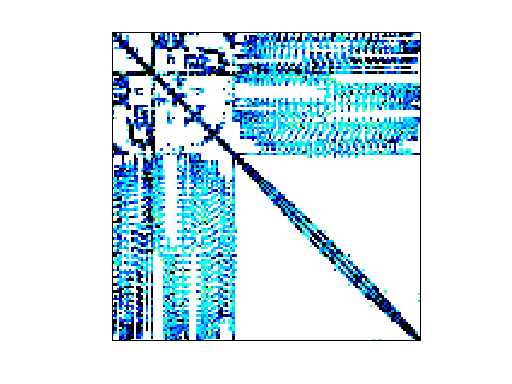
\includegraphics[width=\textwidth]{./images/CG/audi.png}
        \caption{audikw\_1}
    \end{subfigure}
    \quad 
    \begin{subfigure}[b]{0.3\textwidth}
        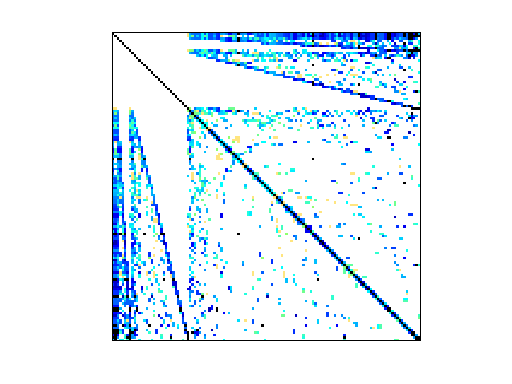
\includegraphics[width=\textwidth]{./images/CG/helm2d03.png}
        \caption{helm2d03}
    \end{subfigure}
    \quad 
	\begin{subfigure}[b]{0.3\textwidth}
        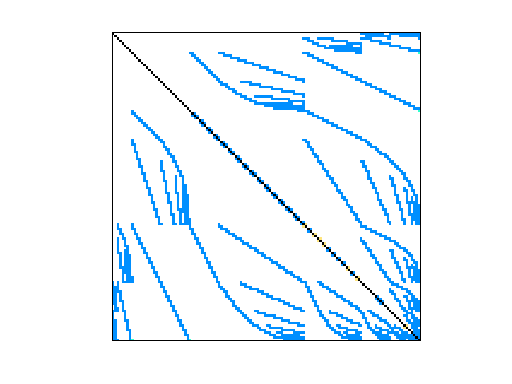
\includegraphics[width=\textwidth]{./images/CG/parabolic_fem.png}
        \caption{parabolic\_fem}
    \end{subfigure}
    \quad 
    \begin{subfigure}[b]{0.3\textwidth}
        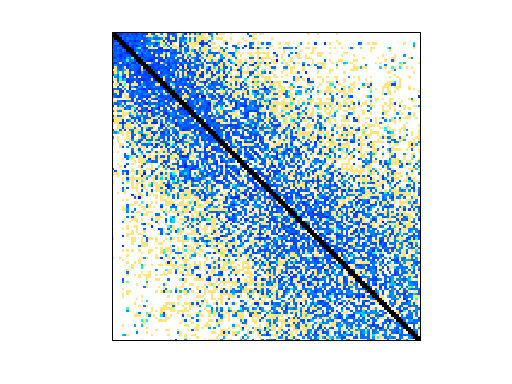
\includegraphics[width=\textwidth]{./images/CG/nd24k.png}
        \caption{nd24k}
    \end{subfigure}
    \quad 
    \begin{subfigure}[b]{0.3\textwidth}
        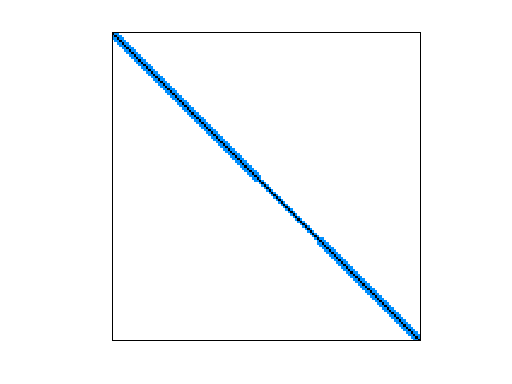
\includegraphics[width=\textwidth]{./images/CG/bone010.png}
        \caption{bone010}
    \end{subfigure}
    \quad 
    \begin{subfigure}[b]{0.3\textwidth}
        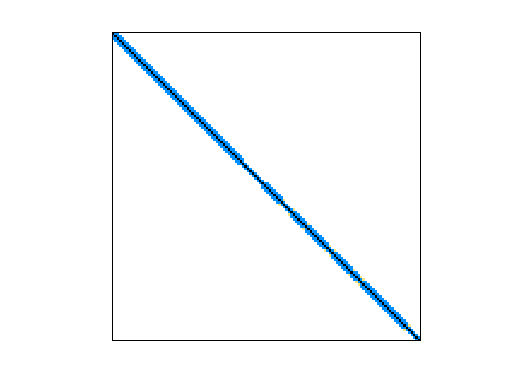
\includegraphics[width=\textwidth]{./images/CG/boneS10.png}
        \caption{boneS10}
    \end{subfigure}
    \quad 
    \begin{subfigure}[b]{0.3\textwidth}
        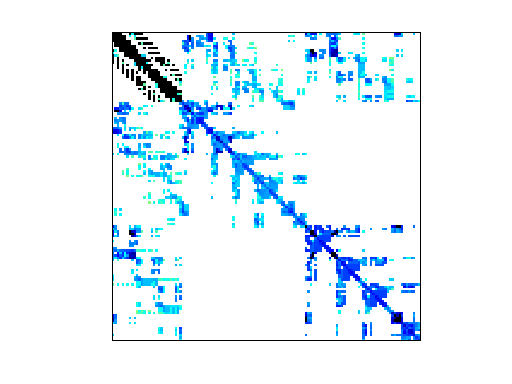
\includegraphics[width=\textwidth]{./images/CG/thread.png}
        \caption{thread}
    \end{subfigure}
    \quad 
    \begin{subfigure}[b]{0.3\textwidth}
        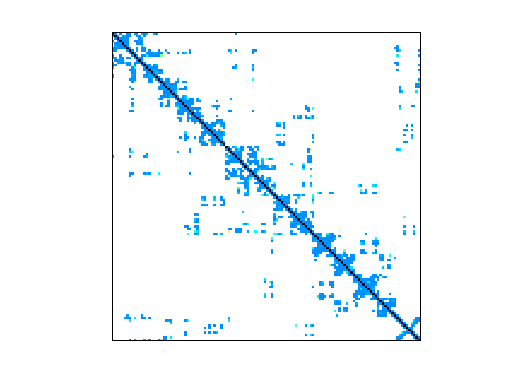
\includegraphics[width=\textwidth]{./images/CG/pdb1HYS.png}
        \caption{pdbHYS}
    \end{subfigure}
    \quad 
    \begin{subfigure}[b]{0.3\textwidth}
        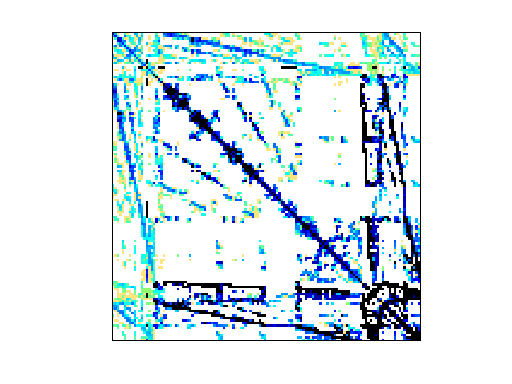
\includegraphics[width=\textwidth]{./images/CG/crankseg_1.png}
        \caption{crankseg\_1}
    \end{subfigure}
    \quad 
    \begin{subfigure}[b]{0.3\textwidth}
        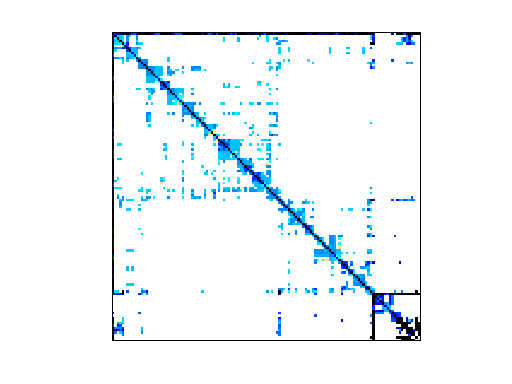
\includegraphics[width=\textwidth]{./images/CG/rajat30.png}
        \caption{rajat30}
    \end{subfigure}
    \quad 
    \begin{subfigure}[b]{0.3\textwidth}
        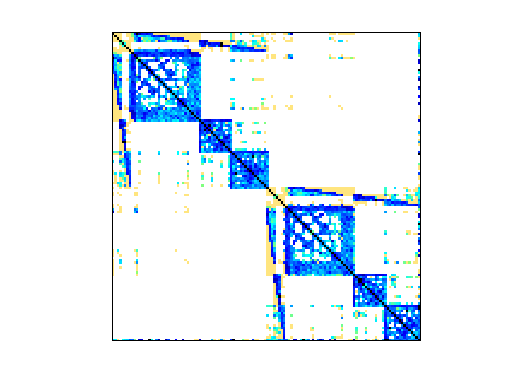
\includegraphics[width=\textwidth]{./images/CG/inline_1}
        \caption{inline\_1}
    \end{subfigure}
    \quad 
    \begin{subfigure}[b]{0.3\textwidth}
        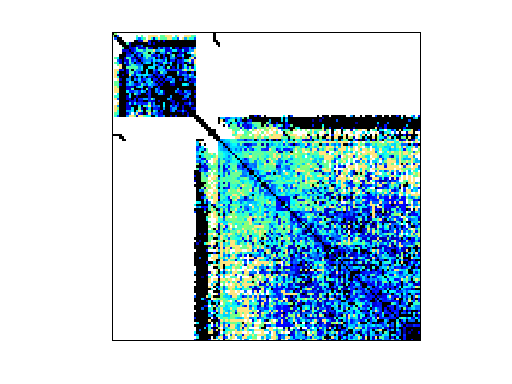
\includegraphics[width=\textwidth]{./images/CG/ldoor.png}
        \caption{ldoor}
    \end{subfigure}
    \quad 
    \begin{subfigure}[b]{0.3\textwidth}
        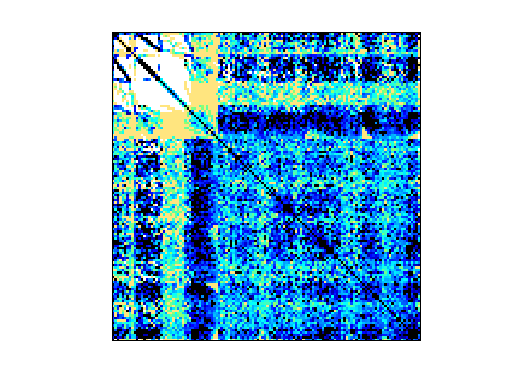
\includegraphics[width=\textwidth]{./images/CG/F1.png}
        \caption{F1}
    \end{subfigure}
    \quad 
    \begin{subfigure}[b]{0.3\textwidth}
        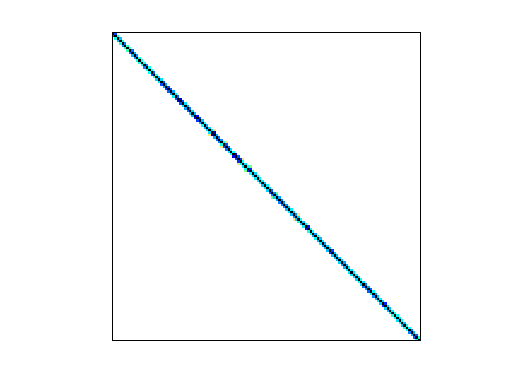
\includegraphics[width=\textwidth]{./images/CG/af_shell9.png}
        \caption{af\_shell9}
    \end{subfigure}
    \quad 
    \begin{subfigure}[b]{0.3\textwidth}
        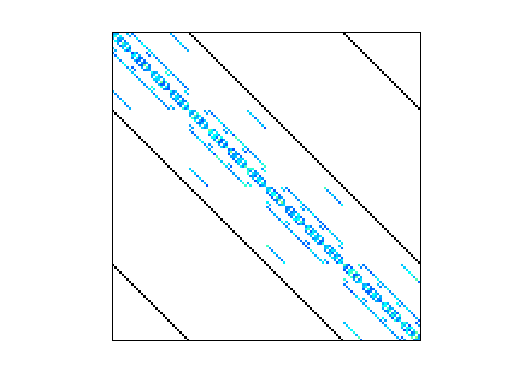
\includegraphics[width=\textwidth]{./images/CG/conf5_0-4x4-26.png}
        \caption{conf5\_0-4x4-26}
    \end{subfigure}
    \quad 
    \begin{subfigure}[b]{0.3\textwidth}
        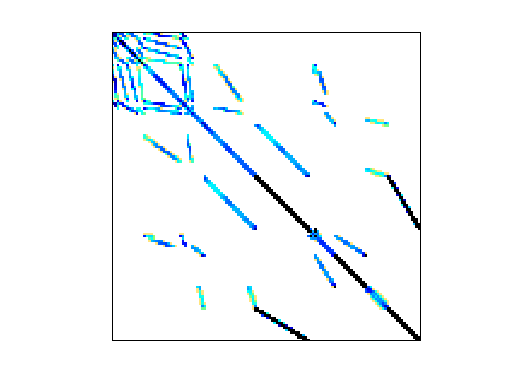
\includegraphics[width=\textwidth]{./images/CG/HV15R.png}
        \caption{HV15R}
    \end{subfigure}
    \quad 
    \caption{Πίνακες εισόδου για το benchmark \textit{p2p\_AS}}
    \label{fig:CG}
\end{figure}

\begin{table}[h]
\centering
\caption{Χαρακτηριστικά πινάκων εισόδου για το benchmark \textit{p2p\_AS}}
\label{table:CG_matrices}
\begin{tabular}{c|c|c}
$Name$ & $Size(\times 10^3)$ & $Non\ Zero\ Values (\times 10^6)$ \\ \hline \hline
audikw\_1 & 943.7 & 77.3 \\
helm2d03 & 392.3 & 2.7 \\
parabolic\_fem & 525.8 & 3.7 \\
nd24k & 72.0 &  28.7 \\
bone010 & 986.7 & 47.9 \\
boneS10 & 914.9 & 40.9 \\
thread & 29.7 & 4.4 \\
pdb1HYS & 36.4 & 4.3 \\
crankseg\_1 & 52.8 & 10.6 \\
rajat30 & 644.0 & 6.2 \\
inline\_1 & 503.7 & 36.8 \\
ldoor & 952.2 & 42.5 \\
F1 & 343.8 & 26.8 \\
af\_shell9 & 504.9 & 17.6\\
conf5\_0-4x4-26 & 3.1 & 0.1 \\
HV15R & 2017.2 & 283.1 \\    
\end{tabular}
\end{table}

\subsection{NB\_SFR}
\paragraph{}
Η ανάπτυξη του benchmark \textit{p2p\_SFR} (point-to-point symmetric with fixed ratio) έγινε με αφορμή την αδυναμία του \textit{p2p\_SRR} να καθορίσει εκ των προτέρων την αναλογία internode και intranode επικοινωνίας. Όπως αναφέραμε, στο benchmark p2p\_SRR κάθε διεργασία επιλέγει τυχαία τη διεργασία που θα ανταλλάξει δεδομένα για κάθε μήνυμα που θα αποστείλει. Ωστόσο, οι τοπικές διεργασίες είναι πολύ λιγότερες από αυτές που βρίσκονται σε άλλο κομβο με αποτέλεσμα, να υπάρχει μεγαλύτερη πιθανότητα να επιλεγούν. Στα περισσότερα σημεία προερχόμενα από p2p\_SRR, η intranode επικοινωνία αποτελούσε περίπου το 25\% της συνολικής επικοινωνίας ανάλογα πάντα και με τον αριθμό των διεργασιών ανά κόμβο. Για την αποφυγή του φαινομένου αυτού, στο benchmark \textit{p2p\_SFR} έχουμε τη δυνατότητα να ορίσουμε εκ των προτέρων την αναλογία intranode και internode επικοινωνίας  επιλέγοντας πόσες διεργασίες ανά κομβό θα επικοινωνούν τοπικά. Το μεγαλύτερο μειονέκτημα του είναι ότι απαιτεί γνώση της αρχιτεκτονικής του μηχανήματος, σε αντίθεση με το \textit{p2p\_SRR}. Ο χώρος παραμέτρων του είναι ο ίδιος με το \textit{p2p\_SRR} με επιπλέον την προσθήκη μίας παραμέτρου εισόδου, $INP$, που ορίζει των αριθμό των διεργασιών που επικοινωνούν εσωτερικά του κόμβου που εκτελούνται, βλ. Πίνακα \ref{table:NBINP}. Τέλος, το benchmark δεν είναι εφαρμόσιμο σε UMA αρχιτεκτονικές αφού δεν λαμβάνει χώρα internode επικοινωνία.

\begin{table}[h]
\centering
\caption{Ο χώρος παραμέτρων για το benchmark \textit{p2p\_SFR}}
\label{table:NBINP}
\begin{tabular}{c|c}
\multirow{1}{*}{Παράμετρος} & \multicolumn{1}{c}{Αρχιτεκτονική} \\ 
                                        & NUMA            \\ \hline \hline
N                                         & 2-4             \\
PPN                                      & 1-8             \\
Size                               & 1B-16MiB        \\
Messages                                & 1-8             \\ 
INP						     & 2/4/6/8(<PPN) \\ \hline
\#samples                               & 8800 \\  \
\end{tabular}
\end{table}



\subsection{Collective}
\paragraph{}
Επιπρόσθετα από τα benchmarks που αφορούσαν την point-to-point επικοινωνία, χρειαστήκαμε και benchmark για την εξαγωγή δειγμάτων εκπαίδευσης για την collective επικοινωνία. Δημιουργήσαμε ξεχωριστά benchmarks για κάθε collective που εξετάσαμε βασισμένοι στα \textit{OSU Micro-Benchmarks}\footnote{http://mvapich.cse.ohio-state.edu/benchmarks/} και τα benchmarks που παρέχει για την collective επικοινωνία του MPI. H αρχική έκδοση των benchmarks, εκτελεί τον τύπο του collective που αφορά, για μερικές εκατοντάδες επαναλήψεις και ένα εύρος από μήκος δεδομένων εισόδου. Για κάθε μήκος επιστρέφει τον μέσο όρο του χρόνου επικοινωνίας από όλες τις επαναλήψεις. Στη δική μας έκδοση, ακολουθούμε το πρότυπο των δύο προηγούμενων benchmarks, όπου ο χρόνος επιλέγεται σαν το μέγιστο κάποιου quantile των τοπικών χρόνων επαναλήψεων και εισάγεται Barrier πριν την έναρξη της επικοινωνίας σε κάθε επανάληψη. Επιλέχθηκε ξανά το τρίτο quantile για τους ίδιους λόγους με το \textit{p2p\_SRR}. O χώρος παραμέτρων δίνεται στον Πίνακα \ref{table:collectives}. Σε αντίθεση με τη point-to-point επικοινωνία, δεν ελέγχαμε το μήκος των μηνυμάτων που ανταλλάσσονται αλλά το μέγεθος των δεδομένων εισόδου \footnote{Στην point-to-point επικοινωνία το μήκος δεδομένων εισόδου ισούται με το μήκος των μηνυμάτων. Κάτι τέτοιο δεν ισχύει σε όλα τα collectives, βλ. Allgather}. Το μήκος των μηνυμάτων εξαρτάται από την υλοποίηση και τον τύπο του collective. 

\begin{table}[h]
\centering
\caption{Ο χώρος παραμέτρων για τα benchmarks \textit{Collective}}
\label{table:collectives}
\begin{tabular}{c|cc}
\multirow{2}{*}{Παράμετρος} & \multicolumn{2}{c}{Αρχιτεκτονική} \\ 
                            & UMA             & NUMA            \\ \hline \hline
N                           & 1               & 2-4             \\
PPN                         & 2-8             & 1-8             \\
Input Size                 & 4B-1MiB     & 4B-1MiB        \\ \hline
\textbf{\#samples}                   & 656              & 2460 
\end{tabular}
\end{table}





\chapter{Πειραματικά Αποτελέσματα Non-Blocking Επικοινωνίας}
\fancyhead[RE,LO]{Πειραματικά Αποτελέσματα Non-Blocking Επικοινωνίας}
%intro needs more work
Σ' αυτό το κεφάλαιο θα παρουσιάσουμε τα πειραματικά αποτελέσματα που αφορούν την Non-Blocking point-to-point επικοινωνία για αρχιτεκτονικές NUMA και UMA. Αρχικά παραθέτουμε τις εφαρμογές και μετρικές που χρησιμοποιήσαμε για να εξετάσουμε τη συμπεριφορά των μοντέλων. Μετέπειτα αναφερόμαστε στα αποτελέσματα και στις προσπάθειες μας για να τα βελτιώσουμε.

\section{Εφαρμογές για εξαγωγή του συνόλου αξιολόγησης}
\paragraph{}
Σε αναλογία με το training set, που προορίζεται για την εκπαίδευση των μοντέλων επικοινωνίας, το σύνολο αξιολόγησης (testing set) περιέχει δείγματα που αποσκοπούν στην εξέταση της ακρίβειας των μοντέλων μας. Εξετάσαμε δύο εφαρμογές, με communication patterns αρκετά συνήθη στις παράλληλες εφαρμογές, για να έχουμε μία γενική εικόνα αναφορικά με τη συμπεριφορά των μοντέλων.
\subsection{3D-Jacobi}
\paragraph{}
Η πρώτη εφαρμογή ήταν μία παράλληλη υλοποίηση της επίλυση ενός προβλήματος διάδοσης θερμότητας σε ένα τρισδιάστατο χωρίο με χρήση της επαναληπτικής μεθόδου Jacobi. Αρχικά, οι MPI διεργασίες τοποθετούνται σε ένα εικονικό 3D καρτεσιανό πλέγμα και με βάση τη θέση τους, το αρχικό χωρίο χωρίζεται σε 3D υποχωρία και κατανέμεται σε αυτές. Κάθε MPI διεργασία έχει, ανάλογα με τη θέση της στο πλέγμα, κάποιες γειτονικές διεργασίες με τις οποίες χρειάζεται να ανταλλάξει δεδομένα.  Συγκεκριμένα, μία διεργασία καλείται να στείλει σε κάθε γειτονική της, τη 2D εδρα που συνορεύει με αυτή βλ. Σχήμα \ref{fig:halo3d}\footnote{http://www.slideshare.net/DevCentralAMD/cc-4005-joshuamora-28493997}. Αντίστοιχα, τον ίδιο όγκο δεδομένων πρέπει να λάβει από αυτές. Αυτού του τύπου μοτίβα επικοινωνίας, όπου γειτονικές διεργασίες με βάση τη κατανομή ενός χωρίου ανταλλάσσουν συμμετρικά δεδομένα, ονομάζονται Halo. Είναι εμφανές ότι το μέγεθος των μηνυμάτων εξαρτάται από τη γεωμετρία του 3D εικονικού πλέγματος και το μέγεθος του αρχικού χωρίου. Σε περίπτωση που το πλέγμα είναι ασύμμετρο, η διάσταση με τις λιγότερες διεργασίες, θα απαιτεί περισσότερη επικοινωνία καθώς οι γειτονικές 2D έδρες είναι μεγαλύτερες. Είχαμε τη δυνατότητα να ορίσουμε τις διαστάσεις του 3D πλέγματος όπως και τις διαστάσεις του αρχικού χωρίου. Πρόκειται για επαναληπτική μέθοδο, με κάθε επανάληψη να εμφανίζει το ίδιο communication pattern και την επικοινωνία που περιγράψαμε. Υπολογίζαμε την πρόβλεψη για μία επανάληψη, $\hat{t}_{iter}$, και την τελική πρόβλεψη μέσω του γινομένου $\hat{t}_{total}= iterations \times \hat{t}_{iter}$. Εκτελέσαμε την εφαρμογή για σωρεία μεγεθών χωρίου και mappings με αποτέλεσμα την εξαγωγή αρκετών σημείων και την πιο σφαιρική αξιολόγηση των μοντέλων. Λεπτομέρειες για τις παραμέτρους εκτέλεσης και τον αριθμό των εξαγόμενων σημείων δίνονται στον Πίνακα \ref{table:par_jacobi}.


\begin{figure}[ht]
    \centering
    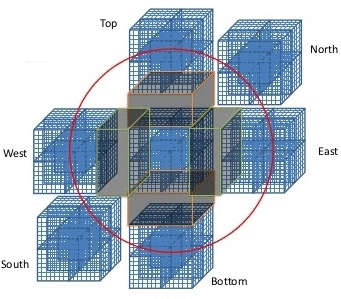
\includegraphics[width=0.55\textwidth]{./images/halo3d.png}
    \caption{Ανταλλαγή Halo-3D}
    \label{fig:halo3d}
\end{figure}
\begin{table} \footnotesize

\centering
\caption{Λεπτομέρειες Εκτέλεσης Jacobi-3D}
\label{table:par_jacobi}
\begin{tabular}{c||c|c}
\multirow{2}{*}{Παράμετρος} & \multicolumn{2}{c}{Αρχιτεκτονική}                                                     \\
                            & UMA                                       & NUMA                                      \\ \hline \hline
N                           & 1                                         & 2-4                                       \\
PPN                         & 2-8                                       & 1-8                                       \\
Domain Size                 & $50^3,100^3,200^3,300^3,400^3,...,1000^3$ & $50^3,100^3,200^3,300^3,400^3,...,1000^3$ \\ 
Iterations                  & 200                                       & 200                                       \\ \hline	
\textbf{\#samples }                  & 66                                        & 176                                      
\end{tabular}
\end{table}





\subsection{LULESH}
\paragraph{}
H δεύτερη εφαρμογή ήταν το Livermore Unstructured Lagrangian Explicit Shock Hydrodynamics (LULESH) \cite{LULESH}. Σε αντίθεση με το 3D-Jacobi, το LULESH παρουσιάζει τρεις φάσεις επικοινωνίας σε κάθε επανάληψη. Η πρώτη φάση, περιλαμβάνει την ανταλλαγή 26 μηνυμάτων, σε ένα 3D-Halo πρότυπο, για την επικοινωνία κάποιων διανυσμάτων δυνάμεων. Η ουσιώδες διαφορά με το 3D-Jacobi είναι ότι τα μηνύματα αυτά δεν είναι ίσου μεγέθους. Η δεύτερη φάση, αφορά την ανταλλαγή μηνυμάτων 6 σημείων, ξανά σε ένα 3D-Halo πρότυπο για την επικοινωνία του ιξώδες του ρευστού, ενώ η τρίτη την επικοινωνία ενός τρισδιάστατου μετώπου κύματος και πάλι 26 σημείων, με θέσεις και ταχύτητες. Προβλέπουμε κάθε μία από αυτές ξεχωριστά, και προσθέτουμε τα αποτελέσματα για να υπολογίσουμε την πρόβλεψη για μία επανάληψη, $\hat{t}_{iter}$. Για την τελική πρόβλεψη,  $\hat{t}$, πολλαπλασιάζουμε το αποτέλεσμα με τον αριθμό των επαναλήψεων. Επιπρόσθετα η MPI υλοποίηση του LULESH εκτελεί ένα \textit{Allreduce} collective για ένα αριθμό κινούμενης υποδιαστολής διπλής ακρίβειας. Με αυτό εξετάζουμε και τη συμπεριφορά των μοντέλων για την collective  επικοινωνία. Λεπτομέρειες για τις παραμέτρους εκτέλεσης δίνονται στον Πίνακα \ref{table:par_lulesh}. Δυστυχώς, η εφαρμογή απαιτεί ο αριθμός των MPI διεργασιών, να είναι αποτέλεσμα κυβικού εκθέτη, γεγονός που περιόριζε τα configurations που μπορούσαμε να εξετάσουμε. Τέλος, σημειώνουμε ότι ο μετρούμενος χρόνος εκτέλεσης, $t$, υπολογίζεται αθροιστικά για κάθε φάση ξεχωριστά, πάνω από όλες τις επαναλήψεις και για τις δύο εφαρμογές.

\begin{table} \footnotesize
\centering
\caption{Λεπτομέρειες Εκτέλεσης LULESH}
\label{table:par_lulesh}
\begin{tabular}{c||c|c}
\multirow{2}{*}{Παράμετρος} & \multicolumn{2}{c}{Αρχιτεκτονική}                                                           \\ 
                            & UMA                                          & NUMA                                         \\ \hline \hline
N                           & 1                                            & 2/4                                          \\
PPN                         & 8                                          & 4/2                                          \\
Domain Size                 & $50^3,60^3,70^3,80^3,90^3,100^3,150^3,200^3$ & $50^3,60^3,70^3,80^3,90^3,100^3,150^3,200^3$ \\
Iterations                  & 200                                          & 200                                          \\ \hline
\textbf{\#samples}                   & 8                                            & 16                                          
\end{tabular}
\end{table}
\section{Μετρικές Αξιολόγησης}
\paragraph{}
Για την αξιολόγηση των μοντέλων μας χρησιμοποιήσαμε τέσσερις μετρικές. Η πρώτη ήταν το σχετικό σφάλμα για κάθε πρόβλεψη, που υπολογίζεται ως ακολούθως:
\begin{align*}
e = \frac{\hat{t}-t}{t}
\end{align*}
Μας έδινε μία αναλυτική εικόνα για τη συμπεριφορά του μοντέλου για κάθε σημείο ξεχωριστά. Έτσι μπορούσαμε να το χρησιμοποιήσουμε για να κάνουμε παρατηρήσεις και να αποφασίσουμε τα επόμενα βήματα της δουλειάς μας.
\paragraph{}
Ωστόσο, καθώς είναι μετρική που υπολογίζεται για την κάθε πρόβλεψη ξεχωριστά χρησιμοποιήσαμε και τη μέση τιμή των απόλυτων τιμών της σαν μετρική αξιολόγησης που μας δίνει μία πιο γενική εικόνα για την ακρίβεια των προβλέψεων. Έστω, $m$ ο αριθμός των προβλέψεων και $e_i$ η τιμή του σχετικού σφάλματος για την i-ιοστή πρόβλεψη. Η μετρική υπολογίζεται ως εξής:
\begin{align*}
\mu = avg(|e_i|), 1\leq i \leq m
\end{align*}
\paragraph{}
Η τρίτη μετρική ήταν το Rank Correlation Coefficient(RCC). Παίρνει τιμές ανάμεσα στο μηδέν και το ένα και ορίζει πόσο καλά προβλέπει το μοντέλο τη διάταξη μεταξύ των μετρούμενων χρόνων. Έτσι, μπορούμε να αποφανθούμε για το κατά πόσο το μοντέλο διακρίνει διαφορές ανάμεσα στα σημεία που προέβλεψε και πόσο καλά θα λειτουργούσε σε σενάρια βελτιστοποίησης. Έστω, $t_i, 1\leq i \leq m$ ο μετρούμενος χρόνος επικοινωνίας και $\hat{t}_i$ η αντίστοιχη πρόβλεψη για m σημεία. Το RCC ορίζεται σαν:
\begin{align*}
RCC = \sum_{1\leq i \leq m} \sum_{1\leq i \leq m} concordant_{ij}/ \frac{m(m-1)}{2}
\end{align*}
όπου,
\begin{align*}
concordant_{ij} = \begin{cases} 
      1, & if \ t_i > t_j \ and \ \hat{t}_i > \hat{t}_j \\
      1, & if \ t_i < t_j \ and \ \hat{t}_i < \hat{t}_j \\
      0, & otherwise  
   \end{cases}
\end{align*}
\paragraph{}
Η τέταρτη, και τελευταία, μετρική αφορά το ποσοστό του πλήθους των προβλέψεων που έχει απόλυτο σφάλμα μικρότερο του 30\%. Τη συμβολίζουμε ως $Pred_{0.30}$ και ορίζεται ως:
\begin{align*}
Pred_{0.30}(\%) = \frac{\#predictions\ with\ |e|\ \leq \ 0.30}{\#predictions} \times 100
\end{align*}

\section{Αποτελέσματα για την αρχιτεκτονική UMA}
\paragraph{}
Τα πρώτα αποτελέσματα που θα παρουσιάσουμε για την point-to-point επικοινωνία αφορούν την αρχιτεκτονική UMA. Η μεγαλύτερη ιδιαιτερότητα της, αναφορικά με τη μεθοδολογία μας, ήταν η απουσία internode επικοινωνίας αφού όλη η επικοινωνία συμβαίνει εντός ενός κόμβου. Κατά συνέπεια, όλες οι μετρικές που την αφορούσα, είχαν μηδενική τιμή, με αποτέλεσμα ο αλγόριθμος εκπαίδευσης του μοντέλου  να τις αγνοεί. Έτσι, σε αυτό το στάδιο δεν χρησιμοποιήσαμε τεχνικές επιλογής χαρακτηριστικών λόγω του μικρού αριθμού μη μηδενικών χαρακτηριστικών.

\subsection{Με δείγματα από το benchmark p2p\_SRR}
\paragraph{}
Η πρώτη μας προσπάθεια για πρόβλεψη έγινε με το training set που εξάγαμε από το Benchmark p2p\_SRR. Ο αλγόριθμος για την εκπαίδευση των μοντέλων επικοινωνίας ήταν, όπως αναφέραμε, o \textit{Gradient Boosting Regressor Tree} του οποίου διατρέξαμε εξαντλητικά τις παραμέτρους για να καταλήξουμε στις καλύτερες δυνατές προβλέψεις. 
\paragraph{}
Στο Σχήμα \ref{fig:NB_jacobi_UMA} φαίνονται τα αποτελέσματα, η κατανομή του απόλυτου σφάλματος, οι παράμετροι εκπαίδευσης και οι μετρικές αξιολόγησης για την εφαρμογή Jacobi-3D. Παρατηρούμε ότι, για τις περιπτώσεις στις οποίες ο χρόνος επικοινωνίας είναι μεγαλύτερος από 250ms, όλες οι προβλέψεις του μοντέλου μας έχουν σφάλμα μικρότερο από 30\%. Ωστόσο, για τις περιπτώσεις στις οποίες ο μετρούμενος χρόνος είναι μικρότερος από 250ms, δίνει προβλέψεις πολύ μικρότερες από τη μετρούμενη τιμή με 60\% των δειγμάτων παρουσιάζουν απόλυτο σφάλμα μικρότερο του 30\%. Εντούτοις, η τιμή του RCC είναι αρκετά ψηλή. Επομένως, προβλέπουμε τη διάταξη των σημείων αρκετά σωστά με κάποιο αρνητικό bias, το οποίο προφανώς δεν οφείλεται σε κακή επιλογή χαρακτηριστικών, αφού τότε δεν θα είχαμε σωστή διάταξη, αλλά σε χρόνους που έχουμε καταγράψει στο training set.

\begin{figure}[ht]
    \centering
    \captionsetup{justification=centering,margin=0cm,font=footnotesize}
    \begin{subfigure}[b]{0.47\textwidth}
        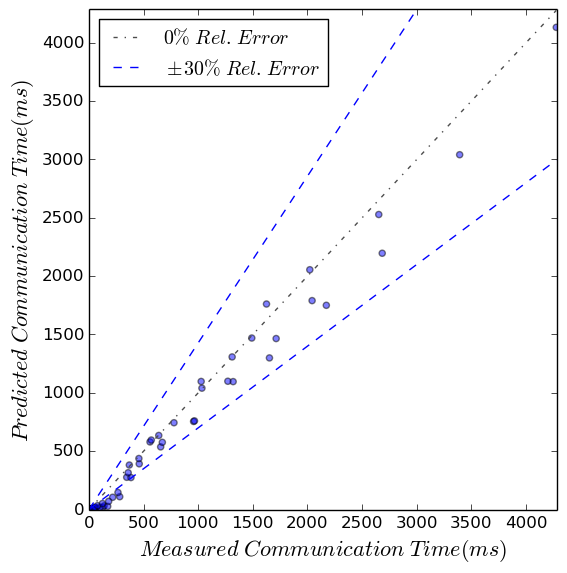
\includegraphics[width=\textwidth]{./images/NB_UMA/NB_jacobi_res.png}
        \caption{Αποτελέσματα}
        \label{fig:NB_jacobi_UMA_res}
    \end{subfigure}
    \quad %add desired spacing between images, e. g. ~, \quad, \qquad, \hfill etc. 
      %(or a blank line to force the subfigure onto a new line)
    \begin{subfigure}[b]{0.47\textwidth}
        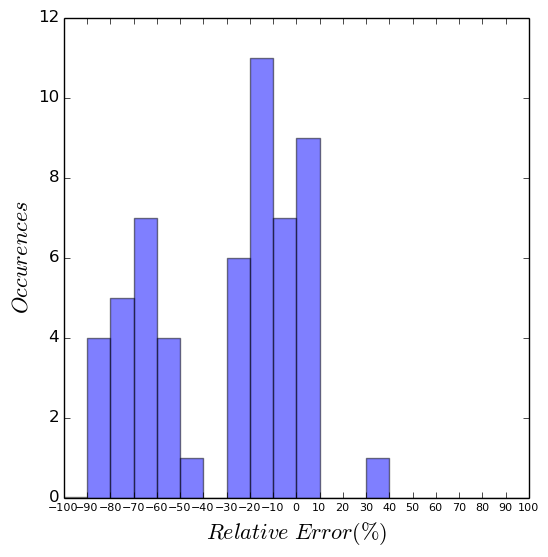
\includegraphics[width=\textwidth]{./images/NB_UMA/NB_jacobi_err_dist.png}
        \caption{Κατανομή Σφάλματος}
        \label{fig:NB_jacobi_UMA_err}
    \end{subfigure} 
    \\[0.2cm]
    \begin{subfigure}[b]{\textwidth}
   	 	\scriptsize
		\begin{tabular}{c||c|c|c|c|c}
			\textbf{Παράμετρος} & n\_estimators & learning\_rate & max\_depth & min\_samples\_leaf & min\_samples\_split \\
			\textbf{Τιμή}       &       100        &  0.1               &  8          &  3                  &    2                 
		\end{tabular}
		\caption{Παράμετροι Μοντέλου}
    \end{subfigure}
    \\[0.2cm]
    \begin{subfigure}[b]{\textwidth}
    		\centering
   	 	\scriptsize
		\begin{tabular}{c||c|c|c}
			\textbf{Μετρική} & $RCC$ &   $avg(|e|)$ & $Pred_{0.3}$  \\
			\textbf{Τιμή}  &  $0.969$   &      $33.278\%
			$        &  $60\%$                                         
		\end{tabular}
		\caption{Μετρικές Αξιολόγησης}
    \end{subfigure}
    
        \caption{Αποτελέσματα, κατανομή σφάλματος, παράμετροι εκπαίδευσης και μετρικές αξιολόγησης για την εφαρμογή Jacobi-3D σε αρχιτεκτονική UMA με το training set του p2p\_SRR}
    \label{fig:NB_jacobi_UMA}
\end{figure}
\paragraph{}
Αναλογικά με την εφαρμογή Jacobi, στο Σχήμα \ref{fig:NB_lulesh_UMA} φαίνονται τα αποτελέσματα για την εφαρμογή LULESH. Η απουσία irregular σημείων στο training set ενισχύει τις ανακρίβειες του μοντέλου για αυτή την εφαρμογή, με 6 από τα 8 χωρία να παρουσιάζουν σφάλμα μεταξύ 80-90\% και το μέσο απόλυτο σφάλμα να αγγίζει το 66.83\%.
\paragraph{}
Η μεγαλύτερη αδυναμία του training set που παράγεται από το p2p\_SRR, είναι ότι όλα τα δείγματα παράγονται μέσω ενός regular communication pattern, με αποτέλεσμα τα μοντέλα που εκπαιδεύουμε να αποτυγχάνουν να διακρίνουν τη διαφορά μεταξύ των ελάχιστων, μέσων και μέγιστων τιμών των μετρικών. Έτσι, τα χαρακτηριστικά που αφορούν ελάχιστες τιμές μετρικών έχουν ίσο ή μεγαλύτερο αντίκτυπο, ανάλογα με τον τρόπο που αναπτύσσεται το μοντέλο, στην τελική πρόβλεψη από αυτά που αντιστοιχούν σε μέσες ή μέγιστες τιμές. Το γεγονός αυτό επιδρά αρνητικά στα μοντέλα μας, καθώς, πιθανότατα, οι μετρικές αυτές, σαν ελάχιστες τιμές, έχουν ελάχιστη συσχέτιση με το χρόνο επικοινωνίας. Για να ξεπεράσουμε αυτό το εμπόδιο, έπρεπε να βρούμε τρόπο να εμπλουτίσουμε το training set που χρησιμοποιούσαμε, με σημεία στα οποία οι ελάχιστες, μέσες και μέγιστες τιμές των μετρικών διαφοροποιούνται. 

\begin{figure}[H]
    \centering
    \captionsetup{justification=centering,margin=0cm,font=footnotesize}
    \begin{subfigure}[b]{0.47\textwidth}
    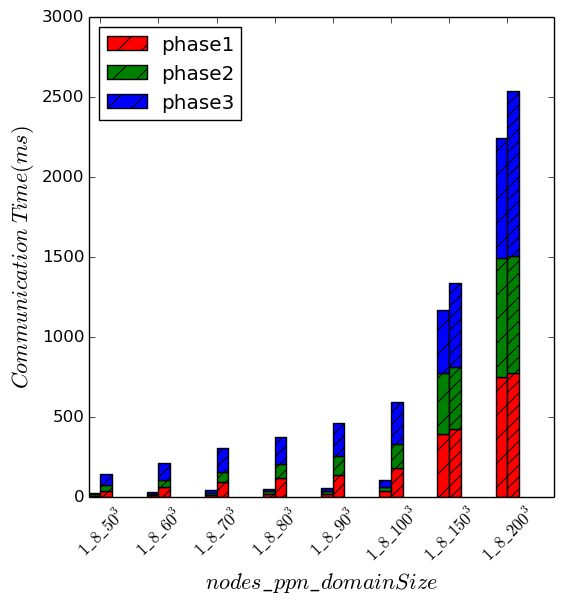
\includegraphics[width=\textwidth]{./images/NB_UMA/NB_lulesh_res.png}
    \caption{Αποτελέσματα}
    \label{fig:NB_lulesh_UMA_res}
    \end{subfigure}
    \quad %add desired spacing between images, e. g. ~, \quad, \qquad, \hfill etc. 
      %(or a blank line to force the subfigure onto a new line)
    \begin{subfigure}[b]{0.47\textwidth}
        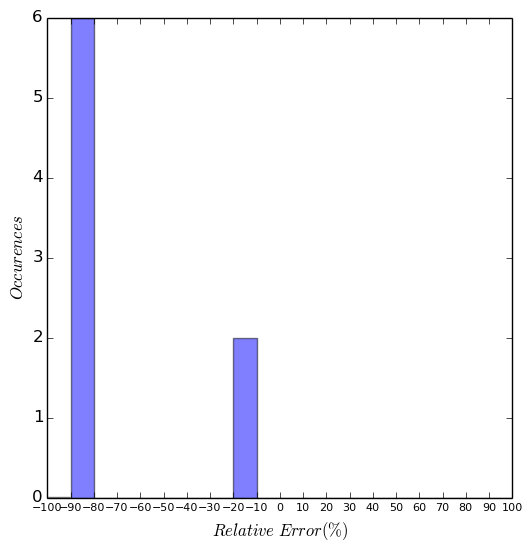
\includegraphics[width=\textwidth]{./images/NB_UMA/NB_lulesh_err_dist.png}
        \caption{Κατανομή Σφάλματος}
        \label{fig:NB_lulesh_UMA_err}
    \end{subfigure}  
    \\[0.2cm]
    \begin{subfigure}[b]{\textwidth}
   	 	\scriptsize
		\begin{tabular}{c||c|c|c|c|c}
			\textbf{Παράμετρος} & n\_estimators & learning\_rate & max\_depth & min\_samples\_leaf & min\_samples\_split \\
			\textbf{Τιμή}       &       100        &  0.1               &  8          &  3                  &    2                 
		\end{tabular}
		\caption{Παράμετροι Μοντέλου}
    \end{subfigure}
    \\[0.2cm]
    \begin{subfigure}[b]{\textwidth}
    		\centering
   	 	\scriptsize
		\begin{tabular}{c||c|c|c}
					\textbf{Μετρική} & $RCC$ &   $avg(|e|)$ & $Pred_{0.3}$  \\
			\textbf{Τιμή}  &  $1.0$   &      $66.83\%
			$        &  $0.25$                                         
		\end{tabular}
		\caption{Μετρικές Αξιολόγησης}
    \end{subfigure}
    \caption{Αποτελέσματα, κατανομή σφάλματος και παράμετροι εκπαίδευσης για την εφαρμογή LULESH σε αρχιτεκτονική UMA με το training set του p2p\_SRR. Οι λεζάντες στον οριζόντιο άξονα των αποτελεσμάτων αντιστοιχούν σε $nodes\_ppn\_$ $domainSize$.}
    \label{fig:NB_lulesh_UMA}
\end{figure}	


\subsection{Με δείγματα από τα Benchmarks p2p\_SRR και p2p\_AS}
\paragraph{}
Για να βελτιώσουμε την ακρίβεια των μοντέλων μας, δημιουργήσαμε το benchmark p2p\_AS και εντάξαμε τα δείγματα εκπαίδευσης που εξάγαμε από αυτό, σε κοινό training set με του p2p\_SRR. Σκοπός μας ήταν, με αυτά τα σημεία να δώσουμε στο μοντέλο μας παραπάνω πληροφορία για διακρίνει τις διαφορές μεταξύ των μετρικών που αποτυγχάνει να διακρίνει μόνο με τα δείγματα εκπαίδευσης του p2p\_SRR, με την εισαγωγή irregular σημείων.

\begin{figure}[ht]
    \centering
    \captionsetup{justification=centering,margin=0cm,font=footnotesize}
    \begin{subfigure}[b]{0.47\textwidth}
        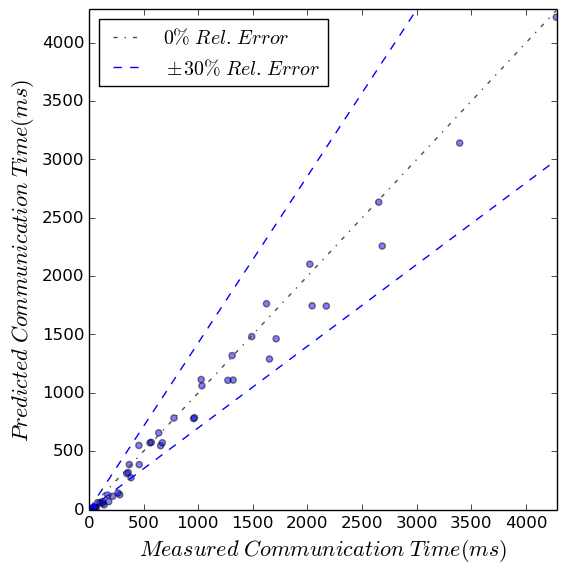
\includegraphics[width=\textwidth]{./images/NB+cg_UMA/NB_cg_jacobi_res.png}
        \caption{Αποτελέσματα}
        \label{fig:NB_cg_jacobi_UMA_res}
    \end{subfigure}
    \quad %add desired spacing between images, e. g. ~, \quad, \qquad, \hfill etc. 
      %(or a blank line to force the subfigure onto a new line)
    \begin{subfigure}[b]{0.47\textwidth}
        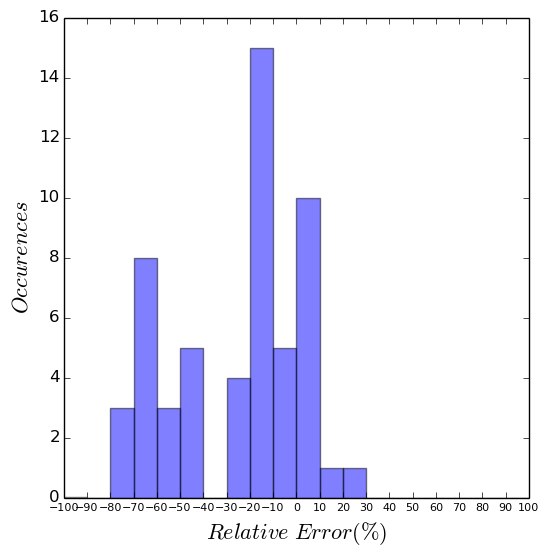
\includegraphics[width=\textwidth]{./images/NB+cg_UMA/NB_cg_jacobi_err_dist.png}
        \caption{Κατανομή Σφάλματος}
        \label{fig:NB_cg_jacobi_UMA_err}
    \end{subfigure} 
    \\[0.3cm]
    \begin{subfigure}[b]{\textwidth}
   	 	\scriptsize
		\begin{tabular}{c||c|c|c|c|c}
			\textbf{Παράμετρος} & n\_estimators & learning\_rate & max\_depth & min\_samples\_leaf & min\_samples\_split \\
			\textbf{Τιμή}       &       200        &  0.1               & 9          &  2                  &    2                 
		\end{tabular}
		\caption{Παράμετροι Μοντέλου}
    \end{subfigure}
    \\[0.3cm]
    \begin{subfigure}[b]{\textwidth}
    		\centering
   	 	\scriptsize
		\begin{tabular}{c||c|c|c}
			\textbf{Μετρική} & $RCC$ &   $avg(|e|)$ & $Pred_{0.3}$  \\
			\textbf{Τιμή}  &  $0.968$   &      $28.642\%
			$        &  $0.65$                                         
		\end{tabular}
		\caption{Μετρικές Αξιολόγησης}
    \end{subfigure}
    
        \caption{Αποτελέσματα, κατανομή σφάλματος, παράμετροι εκπαίδευσης και οι μετρικές αξιολόγησης για την εφαρμογή Jacobi-3D σε αρχιτεκτονική UMA με το training set του p2p\_SRR και του p2p\_AS. }
    \label{fig:NB+cg_jacobi_UMA}
\end{figure}
\paragraph{}
Στο Σχήμα \ref{fig:NB+cg_jacobi_UMA} φαίνονται τα αποτελέσματα, η κατανομή του σφάλματος, οι παράμετροι εκπαίδευσης του μοντέλου εκπαίδευσης και οι μετρικές αξιολόγησης για την εφαρμογή Jacobi-3D και το επεκτεταμένο training set. Παρατηρήσαμε σχετική βελτίωση στις μετρικές αξιολόγησης. Παρόλο που η τιμή του RCC παρέμενε σταθερή, το μοντέλο μας είχε 5\% μικρότερο μέσο όρο απολύτων σφαλμάτων από το προηγούμενο, ενώ τα σημεία που παρουσιάζουν σφάλμα μικρότερο από 30\% αυξάνονται στο από 60\% στο 65\% των δειγμάτων. 


\paragraph{}
Αναλογικά, στο Σχήμα \ref{fig:NB+cg_lulesh_UMA}, φαίνονται τα αντίστοιχα αποτελέσματα για την εφαρμογή LULESH. Πλέον τα σημεία που πριν αποτυγχάνουν δεν παρουσιάζουν σφάλμα 80-90\% αλλά φαίνεται ότι αντιλαμβάνονται καλύτερα τις αλλαγές στην επικοινωνία καθώς μεγαλώνουν τα χωρία της εφαρμογής. Έτσι,το μέσο απόλυτο σφάλμα μειώνεται από 66.83\% στο 53.74\%. 

\begin{figure}[ht]
    \centering
    \captionsetup{justification=centering,margin=0cm,font=footnotesize}
    \begin{subfigure}[b]{0.47\textwidth}
        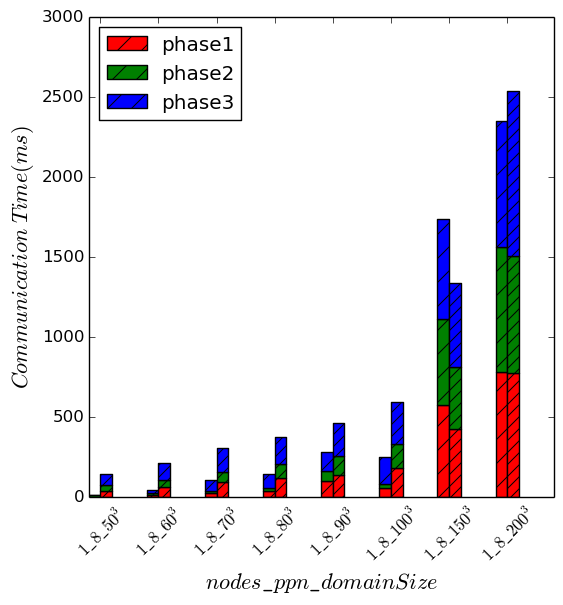
\includegraphics[width=\textwidth]{./images/NB+cg_UMA/NB_cg_lulesh_res.png}
        \caption{Αποτελέσματα}
    \end{subfigure}
    \quad %add desired spacing between images, e. g. ~, \quad, \qquad, \hfill etc. 
      %(or a blank line to force the subfigure onto a new line)
    \begin{subfigure}[b]{0.47\textwidth}
        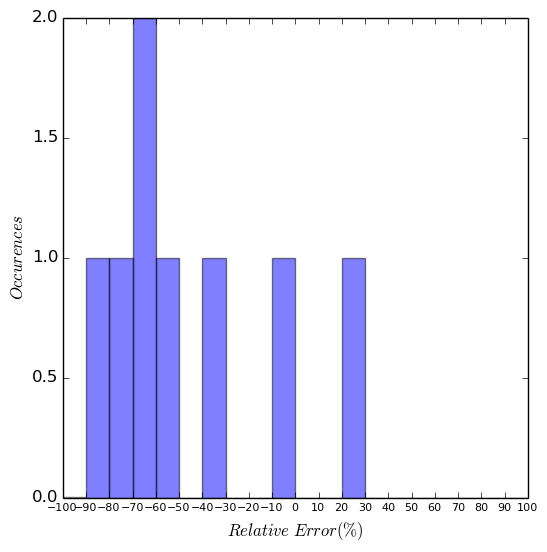
\includegraphics[width=\textwidth]{./images/NB+cg_UMA/NB_cg_lulesh_err_dist.png}
        \caption{Κατανομή Σφάλματος}
    \end{subfigure} 
    \\[0.3cm]
    \begin{subfigure}[b]{\textwidth}
   	 	\scriptsize
		\begin{tabular}{c||c|c|c|c|c}
			\textbf{Παράμετρος} & n\_estimators & learning\_rate & max\_depth & min\_samples\_leaf & min\_samples\_split \\
			\textbf{Τιμή}       &       200        &  0.1               & 9          &  2                  &    2                 
		\end{tabular}
		\caption{Παράμετροι Μοντέλου}
    \end{subfigure}
    \\[0.3cm]
    \begin{subfigure}[b]{\textwidth}
    		\centering
   	 	\scriptsize
		\begin{tabular}{c||c|c|c}
			\textbf{Μετρική} & $RCC$ &   $avg(|e|)$ & $Pred_{0.3}$  \\
			\textbf{Τιμή}  &  $0.964$   &      $53.74\%
			$        &  $25\%$                                         
		\end{tabular}
		\caption{Μετρικές Αξιολόγησης}
    \end{subfigure}
    
        \caption{Αποτελέσματα, κατανομή σφάλματος, παράμετροι εκπαίδευσης και μετρικές αξιολόγησης για την εφαρμογή LULESH σε αρχιτεκτονική UMA με το training set του p2p\_SRR και του p2p\_AS. Οι λεζάντες στον οριζόντιο άξονα των αποτελεσμάτων αντιστοιχούν σε $nodes\_ppn\_$ $domainSize$.}
    \label{fig:NB+cg_lulesh_UMA}
\end{figure}

\paragraph{}
Οφείλουμε να ομολογήσουμε ότι με την εισαγωγή των δειγμάτων από το Benchmark p2p\_AS, αναμέναμε πολύ περισσότερη βελτίωση στην ακρίβεια των μοντέλων μας από αυτή που πετύχαμε. Καταλήξαμε στο συμπέρασμα ότι τα δείγματα του p2p\_AS δεν ήταν αρκετά σε πλήθος, σε σχέση με του p2p\_SRR, για να επηρεάσουν σημαντικά τη συμπεριφορά των μοντέλων καθώς ήταν λιγότερα από το 10\% των ολικών δειγμάτων. Η εξαγωγή περαιτέρω σημείων από τη p2p\_AS κρίθηκε υπερβολικά περίπλοκη, αφού δεν είχαμε άμεση πρόσβαση στις παραμέτρους. Έτσι ακολουθήσαμε άλλες διαδικασίες. Οι περισσότερες δεν απέδωσαν ικανοποιητικά αποτελέσματα και θεωρούμε άσκοπο να τις παρουσιάσουμε. Οι πιο σημαντικές περιελάμβαναν την ανάπτυξη του benchmark p2p\_SFR, στο οποίο είχαμε τη δυνατότητα να ορίσουμε την αναλογία internode και intranode επικοινωνίας καθώς και την τυχαία απόρριψη δειγμάτων από το training set του p2p\_SRR με σκοπό την αύξηση του αντίκτυπου των δειγμάτων του p2p\_AS στο μοντέλο επικοινωνίας. Κάποιες μετρικές αξιολόγησης για αυτές τις μεθόδους δίνονται στο τέλος του κεφαλαίου.
\subsection{Με ρητή επιλογή χαρακτηριστικών}
\paragraph{}
Καθώς ούτε τα αποτελέσματα με το συνδυασμό των δειγμάτων των δύο benchmarks παρουσίαζαν ικανοποιητική επίδοση προσπαθήσαμε να παραλείψουμε χαρακτηριστικά από το training set που πιστεύαμε ότι επηρέαζαν αρνητικά τη συμπεριφορά των μοντέλων. Μετά από αρκετό πειραματισμό καταλήξαμε να κρατάμε στο training set μόνο τα χαρακτηριστικά, \textit{PPN,avgS,avgM,avgPT} και \textit{avgNT}. Τα αποτελέσματα με αυτή τη μέθοδο δίνονται στα Σχήματα \ref{fig:NB+cg_avgonly_jacobi_UMA} και \ref{fig:NB+cg_avgonly_lulesh_UMA}.

\begin{figure}[ht]
    \centering
    \captionsetup{justification=centering,margin=0cm,font=footnotesize}
    \begin{subfigure}[b]{0.47\textwidth}
        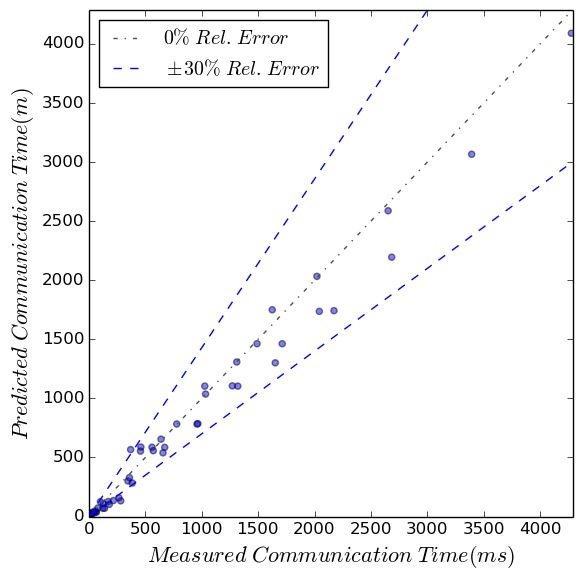
\includegraphics[width=\textwidth]{./images/NB+cg_avgonly_UMA/jacobi_res.png}
        \caption{Αποτελέσματα}
    \end{subfigure}
    \quad %add desired spacing between images, e. g. ~, \quad, \qquad, \hfill etc. 
      %(or a blank line to force the subfigure onto a new line)
    \begin{subfigure}[b]{0.47\textwidth}
        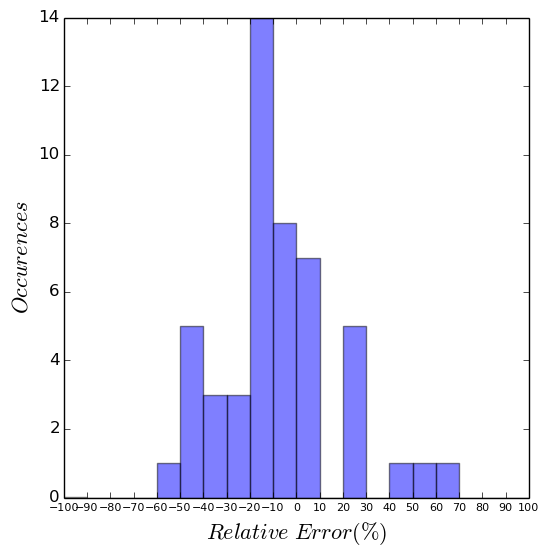
\includegraphics[width=\textwidth]{./images/NB+cg_avgonly_UMA/jacobi_err_dist.png}
        \caption{Κατανομή Σφάλματος}
    \end{subfigure} 
    \\[0.2cm]
    \begin{subfigure}[b]{\textwidth}
   	 	\scriptsize
		\begin{tabular}{c||c|c|c|c|c}
			\textbf{Παράμετρος} & n\_estimators & learning\_rate & max\_depth & min\_samples\_leaf & min\_samples\_split \\
			\textbf{Τιμή}       &       400        &  0.01               & 8          &  3                  &    3                 
		\end{tabular}
		\caption{Παράμετροι Μοντέλου}
    \end{subfigure}
    \\[0.2cm]
    \begin{subfigure}[b]{\textwidth}
    		\centering
   	 	\scriptsize
		\begin{tabular}{c||c|c|c}
			\textbf{Μετρική} & $RCC$ &   $avg(|e|)$ & $Pred_{0.3}$  \\
			\textbf{Τιμή}  &  $0.964$   &      $22.6\%
			$        &  $74\%$                                         
		\end{tabular}
		\caption{Μετρικές Αξιολόγησης}
    \end{subfigure}
    
        \caption{Αποτελέσματα, κατανομή σφάλματος, παράμετροι εκπαίδευσης και μετρικές αξιολόγησης για την εφαρμογή Jacobi-3D σε αρχιτεκτονική UMA με ρητή επιλογή παραμέτρων}
    \label{fig:NB+cg_avgonly_jacobi_UMA}
\end{figure}

\begin{figure}[H]
    \centering
    \captionsetup{justification=centering,margin=0cm,font=footnotesize}
    \begin{subfigure}[b]{0.47\textwidth}
        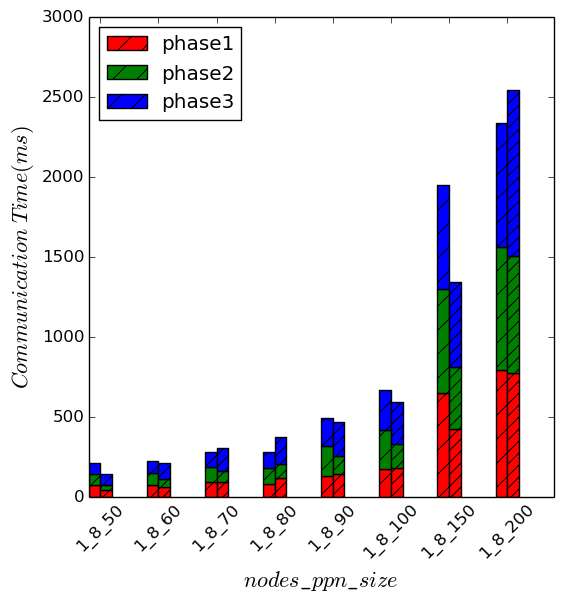
\includegraphics[width=\textwidth]{./images/NB+cg_avgonly_UMA/lulesh_res.png}
        \caption{Αποτελέσματα}
    \end{subfigure}
    \quad %add desired spacing between images, e. g. ~, \quad, \qquad, \hfill etc. 
      %(or a blank line to force the subfigure onto a new line)
    \begin{subfigure}[b]{0.47\textwidth}
        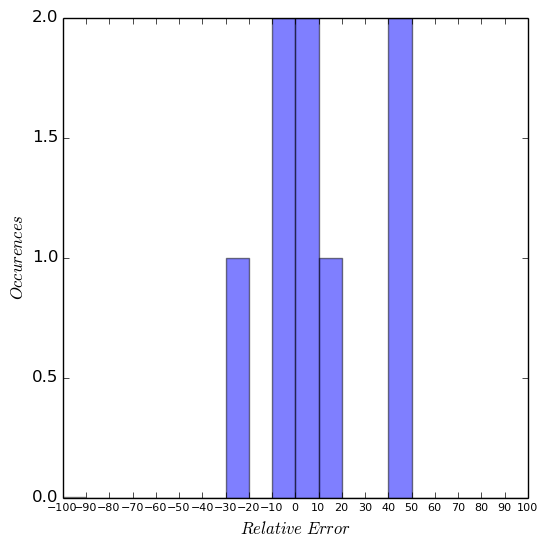
\includegraphics[width=\textwidth]{./images/NB+cg_avgonly_UMA/lulesh_err_dist.png}
        \caption{Κατανομή Σφάλματος}
    \end{subfigure} 
    \\[0.2cm]
    \begin{subfigure}[b]{\textwidth}
   	 	\scriptsize
		\begin{tabular}{c||c|c|c|c|c}
			\textbf{Παράμετρος} & n\_estimators & learning\_rate & max\_depth & min\_samples\_leaf & min\_samples\_split \\
			\textbf{Τιμή}       &       400        &  0.007               & 10          &  1                  &    3                 
		\end{tabular}
		\caption{Παράμετροι Μοντέλου}
    \end{subfigure}
    \\[0.2cm]
    \begin{subfigure}[b]{\textwidth}
    		\centering
   	 	\scriptsize
		\begin{tabular}{c||c|c|c}
			\textbf{Μετρική} & $RCC$ &   $avg(|e|)$ & $Pred_{0.3}$  \\
			\textbf{Τιμή}  &  $0.964$   &      $19.450\%
			$        &  $75\%$                                         
		\end{tabular}
		\caption{Μετρικές Αξιολόγησης}
    \end{subfigure}
    
        \caption{Αποτελέσματα, κατανομή σφάλματος, παράμετροι εκπαίδευσης και μετρικές αξιολόγησης για την εφαρμογή LULESH σε αρχιτεκτονική UMA με ρητή επιλογή παραμέτρων. Οι λεζάντες στον οριζόντιο άξονα των αποτελεσμάτων αντιστοιχούν σε $nodes\_ppn\_domainSize$.}
    \label{fig:NB+cg_avgonly_lulesh_UMA}
\end{figure}

\paragraph{}
Η βελτίωση στα αποτελέσματα είναι προφανής. Για την εφαρμογή Jacobi-3D, το μέσο απόλυτο σφάλμα μειώνεται από 28\% στο 22\%. ενώ περίπου τρία τέταρτα των προβλέψεων παρουσιάζουν σφάλμα μικρότερο από 30\% διατηρώντας ψηλή τιμή για το RCC. Επιπρόσθετα, η εφαρμογή LULESH παρουσίασε τη μεγαλύτερη βελτίωση με την παράλειψη κάποιων μετρικών. Οι μετρικές που κρατήσαμε ήταν οι ίδιες με την εφαρμογή Jacobi-3D. Το μέσο απόλυτο σφάλμα μειώθηκε κατά 34\% με την νέα τιμή να περιοριζόταν στο 19.5\%  ενώ 75\% των προβλέψεων πέτυχαν σφάλμα μικρότερο του 20\%. Αυτές οι προβλέψεις ήταν και οι καλύτερες που καταφέραμε να πετύχουμε.





\section{Αποτελέσματα για την αρχιτεκτονική NUMA}

\paragraph{}
Σε επόμενο στάδιο, αναφερόμαστε στα αποτελέσματα της μεθοδολογίας μας για την αρχιτεκτονική NUMA. Καθώς πλέον λαμβάνει χώρα internode και intranode επικοινωνία ταυτόχρονα, στη γενική περίπτωση όλες οι μετρικές έχουν μη μηδενικές τιμές. Σαν αποτέλεσμα, κάναμε χρήση αλγορίθμων επιλογής χαρακτηριστικών (feature selection) για να αφαιρέσουμε από το training set μετρικές οι οποίες απλά εισήγαγαν θόρυβο και αχρείαστη πληροφορία στο μοντέλο. Η ροή με την οποία παρουσιάζονται τα αποτελέσματα είναι η ίδια με την αρχιτεκτονική UMA, με τα βήματα που ακολουθήσαμε για να καταλήξουμε στα καλύτερα αποτελέσματα. 

\subsection{Με δείγματα από το benchmark p2p\_SRR}
Η πρώτη μας προσπάθεια αφορά τα αποτελέσματα με το training set που εξάγαμε από το benchmark p2p\_SRR. Στα Σχήματα \ref{fig:NB_jacobi_NUMA} και \ref{fig:NB_lulesh_NUMA} παραθέτουμε τα αποτελέσματα για τις δύο εφαρμογές.

\begin{figure}
    \centering
    \captionsetup{justification=centering,margin=0cm,font=footnotesize}
    \begin{subfigure}[b]{0.47\textwidth}
        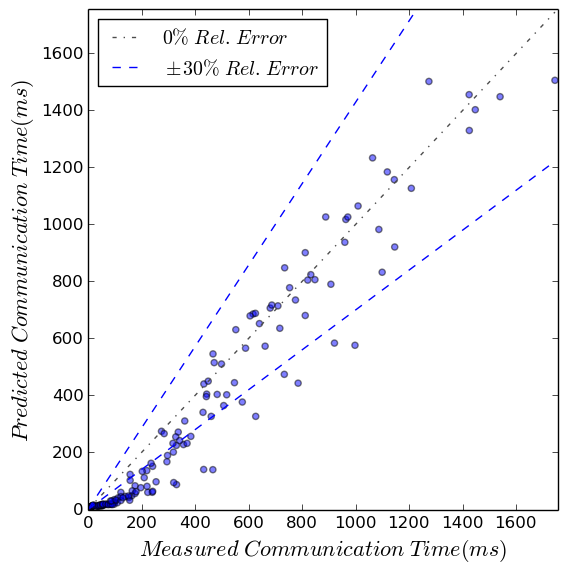
\includegraphics[width=\textwidth]{./images/NB_NUMA/jacobi_res_nfe.png}
        \caption{Αποτελέσματα}
    \end{subfigure}
    \quad %add desired spacing between images, e. g. ~, \quad, \qquad, \hfill etc. 
      %(or a blank line to force the subfigure onto a new line)
    \begin{subfigure}[b]{0.47\textwidth}
        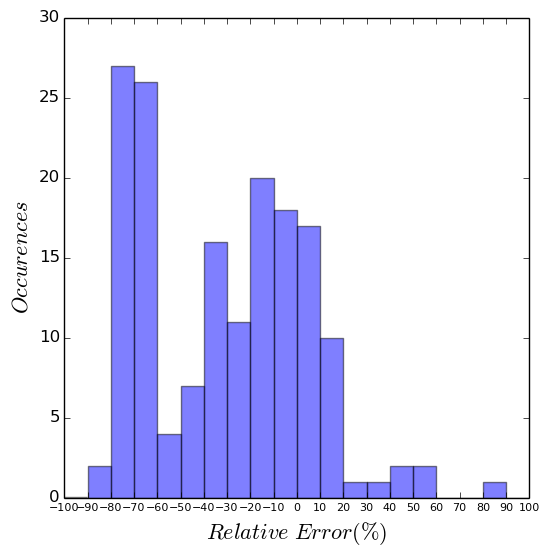
\includegraphics[width=\textwidth]{./images/NB_NUMA/jacobi_err_dist_nfe.png}
        \caption{Κατανομή Σφάλματος}
    \end{subfigure} 
    \\[0.2cm]
    \begin{subfigure}[b]{\textwidth}
   	 	\scriptsize
		\begin{tabular}{c||c|c|c|c|c}
			\textbf{Παράμετρος} & n\_estimators & learning\_rate & max\_depth & min\_samples\_leaf & min\_samples\_split \\
			\textbf{Τιμή}       &       1000        &  0.1               & 10          &  4                  &    2
		\end{tabular}
		\caption{Παράμετροι Μοντέλου}
    \end{subfigure}
    \\[0.2cm]
    \begin{subfigure}[b]{\textwidth}
    		\centering
   	 	\scriptsize
		\begin{tabular}{c||c|c|c}
			\textbf{Μετρική} & $RCC$ &   $avg(|e|)$ & $Pred_{0.3}$  \\
			\textbf{Τιμή}  &  $0.953$   &      $37.398\%
			$        &  $47\%$                                         
		\end{tabular}
		\caption{Μετρικές Αξιολόγησης}
    \end{subfigure}
    
        \caption{Αποτελέσματα, κατανομή σφάλματος, παράμετροι εκπαίδευσης και μετρικές αξιολόγησης για την εφαρμογή Jacobi σε αρχιτεκτονική NUMA με το Benchmark p2p\_SRR}
    \label{fig:NB_jacobi_NUMA}
\end{figure}
\begin{figure}
    \centering
    \captionsetup{justification=centering,margin=0cm,font=footnotesize}
    \begin{subfigure}[b]{0.47\textwidth}
        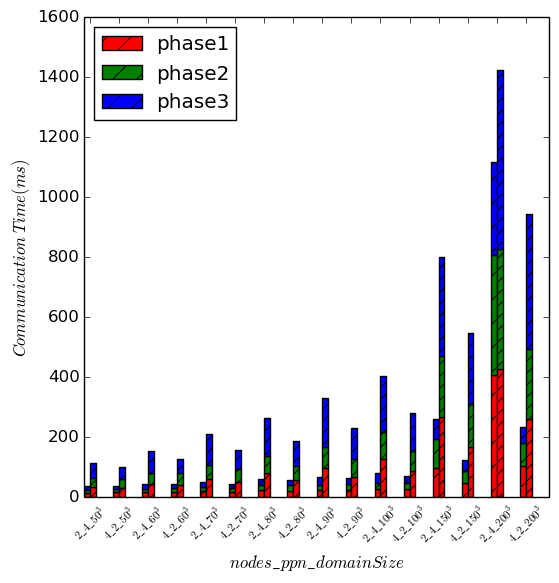
\includegraphics[width=\textwidth]{./images/NB_NUMA/lulesh_res_nfe.png}
        \caption{Αποτελέσματα}
    \end{subfigure}
    \quad %add desired spacing between images, e. g. ~, \quad, \qquad, \hfill etc. 
      %(or a blank line to force the subfigure onto a new line)
    \begin{subfigure}[b]{0.47\textwidth}
        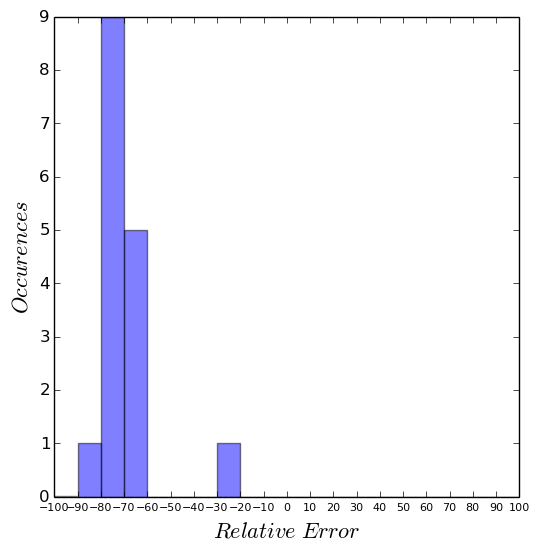
\includegraphics[width=\textwidth]{./images/NB_NUMA/lulesh_err_dist_nfe.png}
        \caption{Κατανομή Σφάλματος}
    \end{subfigure} 
    \\[0.2cm]
    \begin{subfigure}[b]{\textwidth}
   	 	\scriptsize
		\begin{tabular}{c||c|c|c|c|c}
			\textbf{Παράμετρος} & n\_estimators & learning\_rate & max\_depth & min\_samples\_leaf & min\_samples\_split \\
			\textbf{Τιμή}       &       1000        &  0.1               & 10          &  4                  &    2
		\end{tabular}
		\caption{Παράμετροι Μοντέλου}
    \end{subfigure}
    \\[0.2cm]
    \begin{subfigure}[b]{\textwidth}
    		\centering
   	 	\scriptsize
		\begin{tabular}{c||c|c|c}
			\textbf{Μετρική} & $RCC$ &   $avg(|e|)$ & $Pred_{0.3}$  \\
			\textbf{Τιμή}  &  $0.958$   &      $69.42\%
			$        &  $6\%$                                         
		\end{tabular}
		\caption{Μετρικές Αξιολόγησης}
    \end{subfigure}
    
        \caption{Αποτελέσματα, κατανομή σφάλματος, παράμετροι εκπαίδευσης και μετρικές αξιολόγησης για την εφαρμογή LULESH σε αρχιτεκτονική NUMA με το Benchmark p2p\_SRR}
    \label{fig:NB_lulesh_NUMA}
\end{figure}
\paragraph{}
Δυστυχώς, η πρώτη μας προσπάθεια δεν παρουσίαζε ιδιαίτερη ακρίβεια. Αναφορικά με την εφαρμογή Jacobi-3D, μόλις 47\% των προβλέψεων πετύχαιναν απόλυτο σφάλμα μικρότερο του 30\% ενώ το μέσο απόλυτο σφάλμα άγγιζε το 37.4\%. Επιπλέον, 54 από τα 176 δείγματα, παρουσίαζαν σφάλμα 60\% με 80\% με τις προβλέψεις να είναι σημαντικά μικρότερες από τις μετρούμενες τιμές. Επιπλέον, τα αποτελέσματα ήταν απογοητευτικά για την εφαρμογή LULESH, με μόλις μία από τις δεκαέξι προβλέψεις να έχει σφάλμα μικρότερο του 30\% και το μέσω σφάλμα να είναι κοντά στο 70\%. Προσπαθήσαμε να βελτιώσουμε τις προβλέψεις με χρήση μεθόδων feature selection χωρίς ιδιαίτερη επιτυχία, έτσι δεν θα παρουσιάσουμε τα αποτελέσματα τους.

\paragraph{} 
Καταλήψαμε στο συμπέρασμα ότι η ανακρίβεια με τα σημεία εκπαίδευσης του bench\-mark p2p\_SRR οφείλεται σε δύο λόγους. Ο πρώτος, με το μεγάλυτερο αντίκτυπο στις προβλέψεις του LULESH, είναι ξανά η απουσία irregular σημείων από το σύνολο εκπαίδευσης. Ο δεύτερος, αφορά την αναλογία internode και intranode επικοινωνίας που καταλήγουν να εμφανίζουν τα σημεία. Όπως αναφέραμε, στο benchmark p2p\_SRR κάθε διεργασία, επιλέγει τυχαία κάποια άλλη για την ανταλλαγή δεδομένων για κάθε μήνυμα ξεχωριστά. Ωστόσο, η επιλογή αυτή είναι μεν τυχαία αλλά υπάρχει μεγαλύτερη πιθανότητα να επιλεγεί διεργασία για ανταλλαγή, που βρίσκεται σε άλλο κόμβο αφού οι διεργασίες αυτές είναι περισσότερες σε αριθμό. Έτσι, η αναλογία internode και intranode επικοινωνίας σύγκλινε περίπου στο 75\% υπέρ της internode επικοινωνίας ανάλογα πάντα και με το PPN. Αυτός ήταν και ο κύριος λόγος που αναπτύξαμε το benchmark p2p\_SFR που μας έδινε την δυνατότητα να ορίζουμε το επιθυμητό ratio μεταξύ των δύο τύπων επικοινωνίας. Παρόλα αυτά, δεν είχαμε την ανάλογη βελτίωση στα αποτελέσματα.

\subsection{Με δείγματα από τα benchmark p2p\_SRR και p2p\_AS}
\paragraph{}
Μετέπειτα εντάξαμε τα δείγματα από το benchmark p2p\_AS, σε κοινό training set με το p2p\_SRR ακολουθώντας την ίδια συλλογιστική με την UMA αρχιτεκτονική. Εκπαιδεύσαμε μοντέλα με και χωρίς feature selection μεθόδους. Με την ένταξη των σημείων του p2p\_AS στο training set, τα μοντέλα με feature selection παρουσίαζαν μεγαλύτερη ακρίβεια ενώ απαιτούσαν λιγότερο χρόνο για την εκπαίδευσή τους. Τα σχετικά γραφήματα για τις δύο εφαρμογές με feature selection φαίνονται στα Σχήματα \ref{fig:NB_cg_jacobi_NUMA} και \ref{fig:NB_cg_lulesh_NUMA}. Επιπλέον στο Σχήμα \ref{fig:NB_cg_importances} δίνονται τα χαρακτηριστικά που δεν απορρίφθηκαν  και τα αντίστοιχα importances τους στη τελική πρόβλεψη.

\paragraph{}
Από τις γραφικές φαίνεται βελτίωση στη συμπεριφορά των μοντέλων και για τις δύο εφαρμογές. Συγκεκριμένα, αναφορικά με τις μετρικές αξιολόγησης, πετύχαμε 12\% μείωση στο μέσο απόλυτο σφάλμα και αύξηση του $Pred_{0.3}$ στο 67\% για την εφαρμογή Jacobi-3D. Οι προβλέψεις για την εφαρμογή LULESH παρουσιάζουν τεράστια βελτίωση, με το μέσο σφάλμα να μειώνεται κατά 33\% και το $Pred_{0.3}$ αυξάνεται κατά 25\%. Ωστόσο, αποκλίνουν και πάλι αρκετά από τις μετρούμενες τιμές, με μέσο σφάλμα 36.6\%. Από τα importances, παρατηρήσαμε ότι τα πιο σημαντικά χαρακτηριστικά ήταν αυτά που υπολογίζονταν από την κίνηση δεδομένων μεταξύ των κόμβων. Παρόλο που περιμέναμε διαφορές μεταξύ των ελάχιστων, μέσων και μέγιστων χαρακτηριστικών αναμέναμε ότι σε κάθε περίπτωση οι ελάχιστες τιμές θα είχαν ελάχιστο αντίκτυπο στη πρόβλεψη. Ο λόγος που αυτό δεν επιτυγχάνεται, είναι ο ίδιος με την UMA αρχιτεκτονική . Τα δείγματα προερχόμενα από regular communication patterns είναι χιλιάδες, ενώ από irregular εκατοντάδες. Έτσι, η επίδραση τους στο μοντέλο επικοινωνίας είναι περιορισμένη.

\begin{figure}[ht]
    \centering
    \captionsetup{justification=centering,margin=0cm,font=footnotesize}
    \begin{subfigure}[b]{0.47\textwidth}
        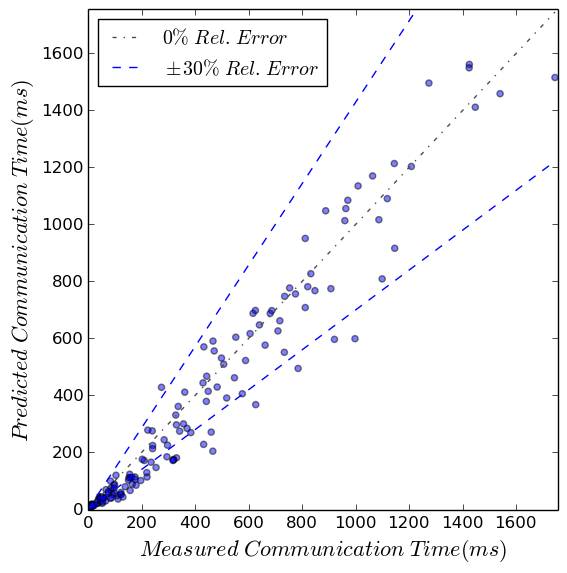
\includegraphics[width=\textwidth]{./images/NB+cg_NUMA/NB_cg_jacobi_res.png}
        \caption{Αποτελέσματα}
    \end{subfigure}
    \quad %add desired spacing between images, e. g. ~, \quad, \qquad, \hfill etc. 
      %(or a blank line to force the subfigure onto a new line)
    \begin{subfigure}[b]{0.47\textwidth}
        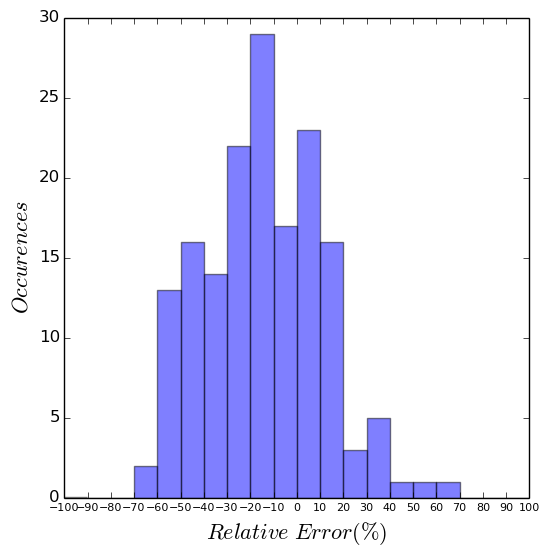
\includegraphics[width=\textwidth]{./images/NB+cg_NUMA/NB_cg_jacobi_err_dist.png}
        \caption{Κατανομή Σφάλματος}
    \end{subfigure} 
    \\[0.2cm]
    \begin{subfigure}[b]{\textwidth}
   	 	\scriptsize
		\begin{tabular}{c||c|c|c|c|c}
			\textbf{Παράμετρος} & n\_estimators & learning\_rate & max\_depth & min\_samples\_leaf & min\_samples\_split \\
			\textbf{Τιμή}       &       2000        &  0.1               & 12          &  3                  &    2
		\end{tabular}
		\caption{Παράμετροι Μοντέλου}
    \end{subfigure}
    \\[0.2cm]
    \begin{subfigure}[b]{\textwidth}
    		\centering
   	 	\scriptsize
		\begin{tabular}{c||c|c|c}
			\textbf{Μετρική} & $RCC$ &   $avg(|e|)$ & $Pred_{0.3}$  \\
			\textbf{Τιμή}  &  $0.947$   &      $25.15\%
			$        &  $67\%$                                         
		\end{tabular}
		\caption{Μετρικές Αξιολόγησης}
    \end{subfigure}
    
        \caption{Αποτελέσματα, κατανομή σφάλματος, παράμετροι εκπαίδευσης και μετρικές αξιολόγησης για την εφαρμογή Jacobi σε αρχιτεκτονική NUMA με τα Benchmarks p2p\_SRR και p2p\_AS}
    \label{fig:NB_cg_jacobi_NUMA}
\end{figure}
\begin{figure}[ht]
    \centering
    \captionsetup{justification=centering,margin=0cm,font=footnotesize}
    \begin{subfigure}[b]{0.47\textwidth}
        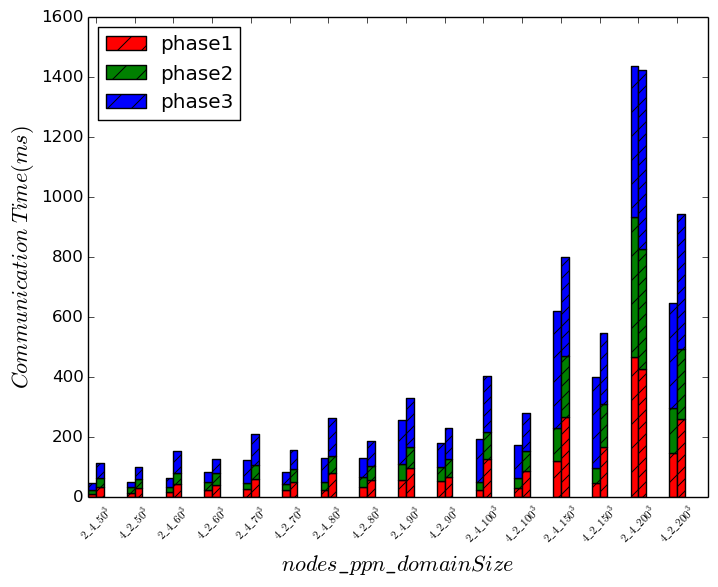
\includegraphics[width=\textwidth]{./images/NB+cg_NUMA/NB_cg_lulesh_res.png}
        \caption{Αποτελέσματα}
    \end{subfigure}
    \quad %add desired spacing between images, e. g. ~, \quad, \qquad, \hfill etc. 
      %(or a blank line to force the subfigure onto a new line)
    \begin{subfigure}[b]{0.47\textwidth}
        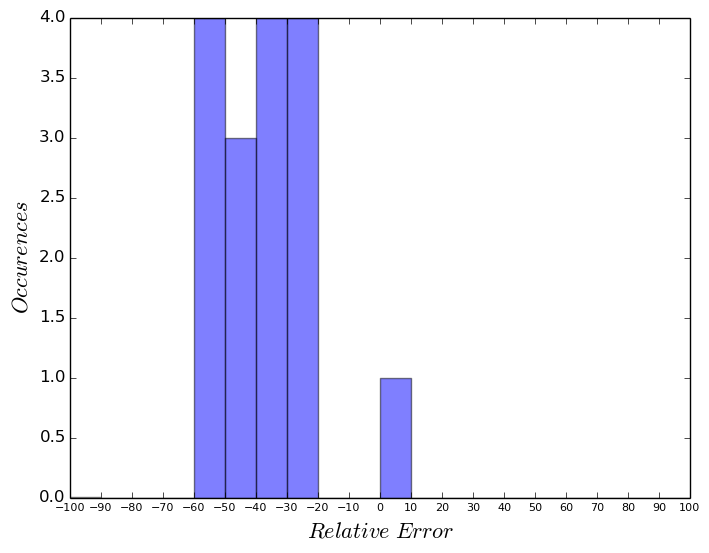
\includegraphics[width=\textwidth]{./images/NB+cg_NUMA/NB_cg_lulesh_err_dist.png}
        \caption{Κατανομή Σφάλματος}
    \end{subfigure} 
    \\[0.2cm]
    \begin{subfigure}[b]{\textwidth}
   	 	\scriptsize
		\begin{tabular}{c||c|c|c|c|c}
			\textbf{Παράμετρος} & n\_estimators & learning\_rate & max\_depth & min\_samples\_leaf & min\_samples\_split \\
			\textbf{Τιμή}       &       2000        &  0.1               & 12          &  3                  &    2
		\end{tabular}
		\caption{Παράμετροι Μοντέλου}
    \end{subfigure}
    \\[0.2cm]
    \begin{subfigure}[b]{\textwidth}
    		\centering
   	 	\scriptsize
		\begin{tabular}{c||c|c|c}
			\textbf{Μετρική} & $RCC$ &   $avg(|e|)$ & $Pred_{0.3}$  \\
			\textbf{Τιμή}  &  $0.950$   &      $36.60\%
			$        &  $31\%$                                         
		\end{tabular}
		\caption{Μετρικές Αξιολόγησης}
    \end{subfigure}
    
        \caption{Αποτελέσματα, κατανομή σφάλματος, παράμετροι εκπαίδευσης και μετρικές αξιολόγησης για την εφαρμογή LULESH σε αρχιτεκτονική NUMA με τα Benchmarks p2p\_SRR και p2p\_AS. Οι λεζάντες στον οριζόντιο άξονα των αποτελεσμάτων αντιστοιχούν σε $nodes\_ppn\_domainSize$.}
    \label{fig:NB_cg_lulesh_NUMA}
\end{figure}

\begin{figure}[H]
    \centering
    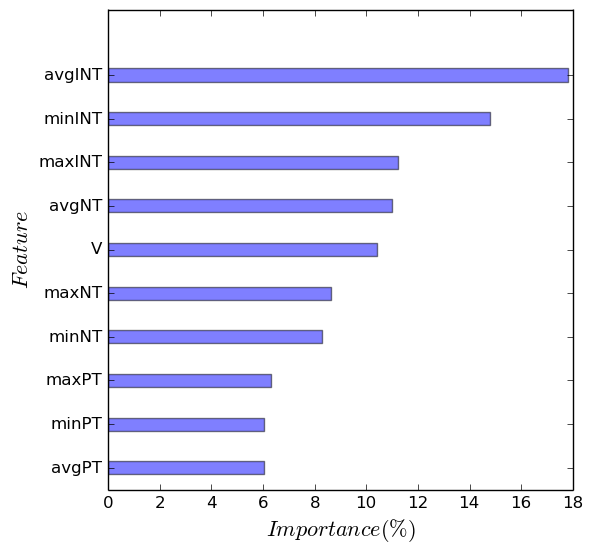
\includegraphics[width=0.7\textwidth]{./images/importance_manually.png}
    \caption{Εναπομείναντα χαρακτηριστικά και τα importances τους}
    \label{fig:NB_cg_importances}
\end{figure}


\subsection{Με ρητή επιλογή χαρακτηριστικών}
\paragraph{}
Καθώς θέλαμε να αυξήσουμε τον αντίκτυπο του \textit{p2p\_AS} στις προβλέψεις, αποφασίσαμε να κάνουμε ρητή επιλογή χαρακτηριστικών με βάση τη διάταξη των importances για ένα μοντέλο εκπαιδευμένο μόνο με το training set του p2p\_AS. Χρησιμοποιώντας τα αποτελέσματα, επιλέγαμε τις μετρικές που θα διατηρούσαμε στο τελικό training set, που περιείχε δείγματα και από τα δύο benchmarks. Στο Σχήμα \ref{fig:importances} δίνονται τα importances για τα δύο training sets. Όπως φαίνεται από στο σχήμα, υπάρχουν σημαντικές διαφορές στην επιρροή των χαρακτηριστικών στην τελική πρόβλεψη. Έτσι, επιβεβαιώνεται ο ισχυρισμός μας, για την αδυναμία του p2p\_AS training set να επηρεάσει το μεγάλο, κοινό training set.

\begin{figure}[ht]
    \centering
    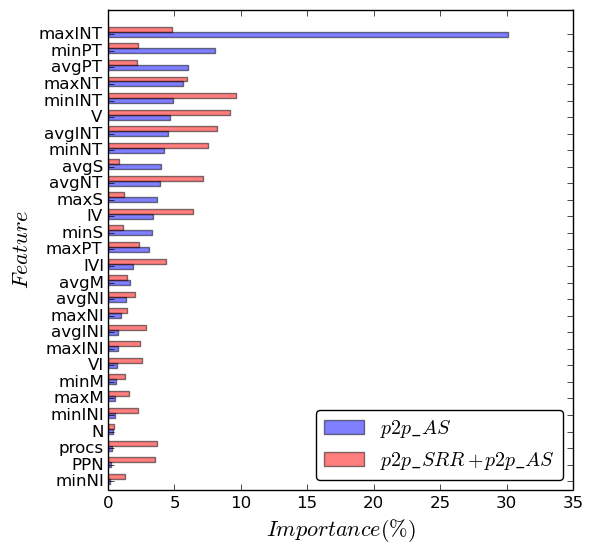
\includegraphics[width=0.7\textwidth]{./images/importance.png}
    \caption{Importances για τα δύο training sets}
    \label{fig:importances}
\end{figure}

\paragraph{}
Οι πιο μεγάλες διαφορές ανάμεσα στα importances αφορούν τις μετρικές NT και ΙΝΤ. Στο p2p\_SRR+p2p\_AS, το minINT είναι το χαρακτηριστικό με το μεγαλύτερο αντίκτυπο στο τελικό αποτέλεσμα. Αντίθετα, στο p2p\_AS, πιο σημαντικό χαρακτηριστικό είναι το maxINT, που αποτελεί διαισθητικά καλύτερη επιλογή καθώς αναμέναμε ότι ο περισσότερος χρόνος επικοινωνίας αναλώνεται για την internode επικοινωνία της εφαρμογής. Επιπρόσθετα, αναφορικά με την INT μετρική, παρατηρούμε μείωση στο importance της ελάχιστης και μέσης τιμής, με τη μέγιστη να μένει αμετάβλητη. Τα χαρακτηριστικά που αφορούν Injection και παραμέτρους εκτέλεσης της εφαρμογής δεν φαίνεται να έχουν ιδιαίτερη επίδραση στο τελικό χρόνο επικοινωνίας με αποτέλεσμα να μην περιλαμβάνονται καθόλου στο τελικό training set, ενώ η μετρική PT είναι η μόνη που διατηρεί την προβληματική συμπεριφορά, με την ελάχιστη τιμή της να έχει μεγαλύτερη σημασία από την μέγιστη.

\paragraph{}
Τα τελικά χαρακτηριστικά που περιλήφθηκαν στο training set ήταν τα $maxS$, $maxPT$, $maxNT$, $maxINT$, $V$ και $IV$. Αποφασίσαμε να αψηφήσουμε το ranking των χαρακτηριστικών για το PT και να συμπεριλάβουμε την μέγιστη τιμή του αντί της ελάχιστης. Τα αναλυτικά αποτελέσματα και για τις δύο εφαρμογές δίνονται στα Σχήματα \ref{fig:NB_cg_mfs_jacobi_NUMA} και \ref{fig:NB_cg_mfs_lulesh_NUMA}
\begin{figure}[ht]
    \centering
    \captionsetup{justification=centering,margin=0cm,font=footnotesize}
    \begin{subfigure}[b]{0.47\textwidth}
        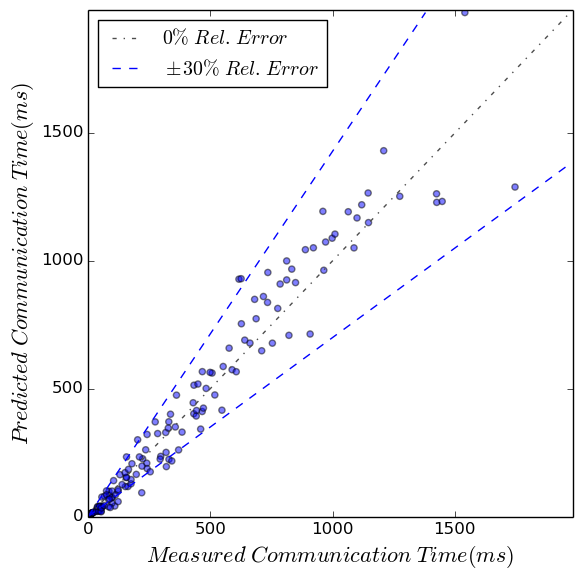
\includegraphics[width=\textwidth]{./images/NB+cg_mfs_NUMA/jacobi_res.png}
        \caption{Αποτελέσματα}
    \end{subfigure}
    \quad %add desired spacing between images, e. g. ~, \quad, \qquad, \hfill etc. 
      %(or a blank line to force the subfigure onto a new line)
    \begin{subfigure}[b]{0.47\textwidth}
        \includegraphics[width=\textwidth]{./images/NB+cg_mfs_NUMA/jacobi_err_dist.png}
        \caption{Κατανομή Σφάλματος}
    \end{subfigure} 
    \\[0.2cm]
    \begin{subfigure}[b]{\textwidth}
   	 	\scriptsize
		\begin{tabular}{c||c|c|c|c|c}
			\textbf{Παράμετρος} & n\_estimators & learning\_rate & max\_depth & min\_samples\_leaf & min\_samples\_split \\
			\textbf{Τιμή}       &       2000        &  0.005          & 10          &  4                  &    5
		\end{tabular}
		\caption{Παράμετροι Μοντέλου}
    \end{subfigure}
    \\[0.2cm]
    \begin{subfigure}[b]{\textwidth}
    		\centering
   	 	\scriptsize
		\begin{tabular}{c||c|c|c}
			\textbf{Μετρική} & $RCC$ &   $avg(|e|)$ & $Pred_{0.3}$  \\
			\textbf{Τιμή}  &  $0.956$   &      $22.116\%
			$        &  $78\%$                                         
		\end{tabular}
		\caption{Μετρικές Αξιολόγησης}
    \end{subfigure}
    
        \caption{Αποτελέσματα, κατανομή σφάλματος, παράμετροι εκπαίδευσης και μετρικές αξιολόγησης για την εφαρμογή Jacobi σε αρχιτεκτονική NUMA με ρητή επιλογή παραμέτρων.}
    \label{fig:NB_cg_mfs_jacobi_NUMA}
\end{figure}
\begin{figure}[H]
    \centering
    \captionsetup{justification=centering,margin=0cm,font=footnotesize}
    \begin{subfigure}[b]{0.47\textwidth}
        \includegraphics[width=\textwidth]{./images/NB+cg_mfs_NUMA/lulesh_res.png}
        \caption{Αποτελέσματα}
    \end{subfigure}
    \quad %add desired spacing between images, e. g. ~, \quad, \qquad, \hfill etc. 
      %(or a blank line to force the subfigure onto a new line)
    \begin{subfigure}[b]{0.47\textwidth}
        \includegraphics[width=\textwidth]{./images/NB+cg_mfs_NUMA/lulesh_err_dist.png}
        \caption{Κατανομή Σφάλματος}
    \end{subfigure} 
    \\[0.2cm]
    \begin{subfigure}[b]{\textwidth}
   	 	\scriptsize
		\begin{tabular}{c||c|c|c|c|c}
			\textbf{Παράμετρος} & n\_estimators & learning\_rate & max\_depth & min\_samples\_leaf & min\_samples\_split \\
			\textbf{Τιμή}       &       2000        &  0.002               & 10          &  4                  &    5
		\end{tabular}
		\caption{Παράμετροι Μοντέλου}
    \end{subfigure}
    \\[0.2cm]
    \begin{subfigure}[b]{\textwidth}
    		\centering
   	 	\scriptsize
		\begin{tabular}{c||c|c|c}
			\textbf{Μετρική} & $RCC$ &   $avg(|e|)$ & $Pred_{0.3}$  \\
			\textbf{Τιμή}  &  $0.975$   &      $12.05\%
			$        &  $100\%$                                         
		\end{tabular}
		\caption{Μετρικές Αξιολόγησης}
    \end{subfigure}
    
        \caption{Αποτελέσματα, κατανομή σφάλματος, παράμετροι εκπαίδευσης και μετρικές αξιολόγησης για την εφαρμογή LULESH σε αρχιτεκτονική NUMA με ρητή επιλογή παραμέτρων. Οι λεζάντες στον οριζόντιο άξονα των αποτελεσμάτων αντιστοιχούν σε $nodes\_ppn\_domainSize$.}
    \label{fig:NB_cg_mfs_lulesh_NUMA}
\end{figure}

\paragraph{}
Η ακρίβεια και η συμπεριφορά των τελευταίων μοντέλων ξεπερνά όλες τις προηγούμενές μας προσπάθειες. Για την εφαρμογή Jacobi, καταφέραμε να βελτιώσουμε όλες τις μετρικές αξιολόγησης με σχεδόν 80\% των προβλέψεων να παρουσιάζουν απόλυτο σφάλμα μικρότερο από 30\%. Επιπρόσθετα, μεγάλη βελτίωση παρουσιάζεται για την εφαρμογή LULESH. Το μέσο απόλυτο σφάλμα μειώνεται από 36.6\% στο 12.05\% με όλες τις προβλέψεις να παρουσιάζουν απόλυτο σφάλμα μικρότερο από 30\%. Σ' αυτό το σημείο, θεωρήσαμε ότι περαιτέρω βελτίωση της μεθοδολογίας δεν ήταν απαραίτητη.

\section{Συνολική Αξιολόγηση}
\paragraph{}
Στους Πίνακες \ref{table:metrics_jacobi} και \ref{table:metrics_lulesh} δίνονται οι μετρικές αξιολόγησης για όλους τους συνδυασμούς training sets που μας απασχόλησαν, συμπεριλαμβανομένων αυτών που δεν παρουσιάσαμε αναλυτικά πιο πάνω. Συγκεκριμένα οι επιπλέον μετρικές αφορούν το training set από το benchmark \textit{p2p\_SFR} και το training set με την τυχαία επιλογή 30\% των δειγμάτων από το \textit{ΝΒ\_p2p} και όλα τα δείγματα προερχόμενα από το \textit{p2p\_AS}. Σημειώνουμε ότι, το benchmark \textit{p2p\_SFR} δεν είναι εφαρμόσιμο στη UMA αρχιτεκτονική καθώς δεν υπάρχει διάκριση ανάμεσα σε intranode και internode επικοινωνία. Επιπρόσθετα, η τεχνική της τυχαίας επιλογής του 30\% δεν κρίθηκε κατάλληλη για την UMA αρχιτεκτονική λόγω του μικρού πλήθους των δειγμάτων.
\begin{table}[h]
\captionsetup{justification=centering,margin=0cm}

\centering
\footnotesize
\caption{Μετρικές αξιολόγησης για όλες τις μεθόδους και αρχιτεκτονικές για την εφαρμογή Jacobi}
\label{table:metrics_jacobi}
\begin{tabular}{c|ccc|ccc}
\multirow{2}{*}{Training Set Source} &   \multicolumn{3}{c}{UMA}    & \multicolumn{3}{c}{NUMA}            \\
         & $RCC$ & $avg(|e|)$ & $Pred_{0.3}$ & $RCC$ & $avg(|e|)$ & $Pred_{0.3}$  \\ \hline \hline
p2p\_SRR & $0.969$ & $33.278\%$ & $60\%$ & $ 0.953 $ & $ 37.398\% $ & $ 47\% $ \\
p2p\_SRR+p2p\_AS & $0.968$ & $28.642\%$ & $65\%$ & $ 0.947 $  & $ 25.15\% $ & $67\%$ \\                   
p2p\_SFR+p2p\_AS & N/A & N/A & N/A & $ 0.943 $ & $ 30.9\% $  & $54\%$ \\
(0.3 $\times$ p2p\_SRR) + p2p\_AS & N/A & N/A & N/A & $ 0.946 $  & $ 23.389\% $ & $ 67\%$ \\ 
Explicit feature selection & $ 0.964 $ & $ 22.6\% $ & $ 74\% $ & $ 0.956 $ & $ 22.12\% $ & $ 78\% $
\end{tabular}
\end{table}


\begin{table}[h]
\centering
\footnotesize
\captionsetup{justification=centering,margin=0cm}
\caption{Μετρικές αξιολόγησης για όλες τις μεθόδους και αρχιτεκτονικές για την εφαρμογή Lulesh}
\label{table:metrics_lulesh}
\begin{tabular}{c|ccc|ccc}
\multirow{2}{*}{Training Set Source} &                              \multicolumn{3}{c}{UMA}             & \multicolumn{3}{c}{NUMA}            \\
         & $RCC$ & $avg(|e|)$ & $Pred_{0.3}$ & $RCC$ & $avg(|e|)$ & $Pred_{0.3}$  \\ \hline \hline
p2p\_SRR & $1.0$ & $66.83\%$ & $25\%$ & $ 0.958 $ & $ 69.42\% $  & $ 6\% $\\
p2p\_SRR+p2p\_AS & $0.964$ & $53.74\%$ & $25\%$ & $0.950$ & $36.60\% $ & $ 31\% $ \\                   
p2p\_SFR+p2p\_AS & N/A & N/A & N/A & $0.875$ & $45.25\%$ & $31\%$ \\
(0.3 $\times$ p2p\_SRR) + p2p\_AS & N/A & N/A & N/A & $0.942 $ & $33.861\% $ & $0.38\% $ \\ 
Explicit feature selection & $0.964$ & $ 19.45\% $ & $ 75\% $ & $0.975$ & $ 12.05\% $ & $100\%$ 
\end{tabular}
\end{table}

\paragraph{}
Όσο αφορά το training set με σημεία από τα benchmarks \textit{p2p\_SFR} και \textit{p2p\_AS}, παρατηρήσαμε μείωση της ακρίβειας των μοντέλων με τη χρήση του σε σχέση με τα προηγούμενα. Πιστεύαμε, ότι με το benchmark αυτό θα ξεπερνούσαμε κάποιες από τις αδυναμίας του benchmark p2p\_SRR. Παρόλα αυτά, το p2p\_SRR, λόγω του  communication pattern που υλοποιεί, μπορεί να δώσει στα μοντέλα μας μια πιο ολοκληρωμένη εικόνα για την επικοινωνία ενώ φαίνεται ότι ο αλγόριθμος GBRΤ μπορεί να αντιμετωπίσει αποτελεσματικά το πρόβλημα με το ratio της internode και intranode επικοινωνίας.

\paragraph{} 
Στην προσπάθειά μας να αυξήσουμε τον αντίκτυπο του benchmark \textit{p2p\_AS} στις τελικές προβλέψεις σκεφτήκαμε να απορρίψουμε τυχαία κάποια σημεία του \textit{p2p\_SRR} από το training set, με σκοπό ο αριθμός των σημείων των δύο benchmarks να είναι συγκρίσιμος. Για την εφαρμογή Jacobi, παρατηρήσαμε σημαντική βελτίωση, ενώ για την εφαρμογή LULESH μικρότερη. Το μεγαλύτερο μειονέκτημα της μεθόδου αυτής ήταν η έλλειψη κανονικότητας. Καθώς η απόρριψη των σημείων ήταν τυχαία, με κάθε εκπαίδευση του μοντέλου οι προβλέψεις διαφέρουν. Έτσι, ένα μοντέλο με το ίδιο training set(πριν την απόρριψη των σημείων), και τις ίδιες παραμέτρους εκπαίδευσης, μπορούσε να δίνει καλές και κακές προβλέψεις ανάλογα με τα δείγματα που απομένουν στο τελικό training set. 




\chapter{Πειραματικά Αποτελέσματα Collective Επικοινωνίας}
\fancyhead[RE,LO]{Πειραματικά Αποτελέσματα Collective Επικοινωνίας}
Σε αυτό το κεφάλαιο παρουσιάζουμε τα αποτελέσματα για την collective επικοινωνία για τις αρχιτεκτονικές NUMA και UMA. Θα παρουσιάσουμε τα αποτελέσματα για μερικά από τα collectives ξεχωριστά παραλείποντας τα collectives που έχουν παρόμοιες υλοποιήσεις. Συγκεκριμένα, θα περιοριστούμε στην αναλυτική παρουσίαση των \textit{scatter}, \textit{bcast} και \textit{allreduce} και στο τέλος θα παραθέσουμε συνοπτικά τα αποτελέσματα για τα υπόλοιπα collectives.  Για όλα τα collectives αναπτύσσεται κοινό μοντέλο επικοινωνίας. Ωστόσο, για την βελτίωση των αποτελεσμάτων προσθέσαμε στα χαρακτηριστικά ένα tag, που αντιπροσωπεύει το collective, έτσι ώστε το μοντέλο μας να μπορεί να ξεχωρίσει το τύπο collective που προσπαθούσαμε να προβλέψουμε. Μπορούσαμε ισοδύναμα, να εκπαιδεύσουμε ξεχωριστά μοντέλα για κάθε τύπο collective αλλά θεωρήσαμε την επιλογή μας πιο εύχρηστη. Στο τέλος του κεφαλαίου παραθέτουμε επίσης, τις προβλέψεις για το collective \textit{allreduce} που χρησιμοποιεί η εφαρμογή LULESH.

\section{Scatter}
\paragraph{}
Ξεκινώντας από την UMA αρχιτεκτονική, στο Σχήμα \ref{fig:scatter_sizes} φαίνονται οι προβλέψεις για το collective scatter με σταθερό μέγεθος\footnote{Σε όλες τις περιπτώσεις με το μέγεθος αναφερόμαστε στο μήκος των κομματιών που σπάει ο μεγάλος buffer εισόδου} και διάφορους ζητούμενους πόρους. Σημειώνουμε ότι, σε αυτές τις προβλέψεις το training και το testing set ήταν τα ίδια. Σκοπός μας ήταν να αξιολογήσουμε κατά πόσο το μοντέλο καταφέρνει με το training set , που βασίζεται στο αφηρημένο communication pattern που αναπτύξαμε, να δώσει ρεαλιστικές προβλέψεις (self-validation) . Από τα αποτελέσματα παρατηρούμε ότι, αν εξαιρέσουμε κάποια ελάχιστα σφάλματα για τα μηνύματα μεγέθους 1KiB, το μοντέλο προβλέπει σωστά τους χρόνους επικοινωνίας. 
\paragraph{}
Επίσης, ενδιαφέρον έχει και ο τρόπος που ο χρόνος επικοινωνίας κλιμακώνει. Για μέγεθος 1KiB και PPN 4,6 και 8 η επικοινωνία κλιμακώνει. Το working set του benchmark χωράει στην κρυφή μνήμη, με την επικοινωνία να μην επηρεάζεται καθόλου από τη κύρια μνήμη και να εκμεταλλεύεται πλήρως το ψηλό bandwidth του διαδρόμου. Για τα δύο επόμενα μεγέθη ο χρόνος επικοινωνίας αυξάνει σχετικά γραμμικά με την αύξηση των πόρων.  Αντίθετα για το μεγαλύτερο μήνυμα που εξετάσαμε, 1MiB, παρατηρούμε μη γραμμική αύξηση στο χρόνο επικοινωνίας καθώς ο μεγάλος όγκος των δεδομένων πιέζει όλο και περισσότερα τμήματα της αρχιτεκτονικής του συστήματος. Ωστόσο, ο μεγαλύτερος χρόνος επικοινωνίας παραμένει μικρότερος από 4ms.
\paragraph{}
Επιπλέον, στο Σχήμα \ref{fig:scatter_conf} φαίνονται οι χρόνοι και οι προβλέψεις για κάποια configu\-rations και όλα τα μεγέθη μηνυμάτων που εξετάσαμε. Σε αναλογία με το προηγούμενο σχήμα, το μοντέλο μας καταφέρνει να κάνει ακριβείς προβλέψεις. Αυτό που ξεχωρίζει από το σχήμα είναι ότι ο χρόνος επικοινωνίας για τα μηνύματα μήκους μικρότερου από 2KiB είναι σχετικά σταθερός. Μετά από μια απότομη μεταβολή στους χρόνους από τα 2KiB στα 4KiB ο χρόνος ξεκινά και αυξάνει με το μέγεθος του μηνύματος.
\begin{figure}[H]
    \centering
    \captionsetup{justification=centering,margin=0cm}
    \begin{subfigure}[b]{0.45\textwidth}
        \includegraphics[width=\textwidth]{./images/scatter/scatter_1024}
        \caption{1KiB}
    \end{subfigure}
    \quad 
        \begin{subfigure}[b]{0.45\textwidth}
        \includegraphics[width=\textwidth]{./images/scatter/scatter_16384}
        \caption{16KiB}
    \end{subfigure}
    \quad
        \begin{subfigure}[b]{0.45\textwidth}
        \includegraphics[width=\textwidth]{./images/scatter/scatter_262144}
        \caption{256KiB}
    \end{subfigure}
    \quad
        \begin{subfigure}[b]{0.45\textwidth}
        \includegraphics[width=\textwidth]{./images/scatter/scatter_1048576}
        \caption{1MiB}
    \end{subfigure}

    \caption{Αποτελέσματα scatter για σταθερό μέγεθος μηνύματος σε αρχιτεκτονική UMA}
        \label{fig:scatter_sizes}
\end{figure}
\begin{figure}[H]
    \centering
    \includegraphics[width=0.65\textwidth]{./images/scatter/scatter.png}
    \caption{Αποτελέσματα scatter για μερικά configurations σε αρχιτεκτονική UMA}
    \label{fig:scatter_conf}
\end{figure}


\paragraph{}
Όπως και για την UMA αρχιτεκτονική, στο Σχήμα \ref{fig:scatter_sizes_NUMA} δίνονται οι προβλέψεις για σταθερός μήκος μηνύματος και μεταβαλλόμενο μέγεθος των δεσμευμένων πόρων, ενώ στο Σχήμα \ref{fig:scatter_conf_NUMA} δίνονται οι προβλέψεις για όλα τα μεγέθη μηνύματος και για μερικά configurations. Η γενική εικόνα σχετικά με τις προβλέψεις παραμένει η ίδια, με το μοντέλο μας να επιδεικνύει πολύ καλή συμπεριφορά. Σε αντιδιαστολή με την αρχιτεκτονική UMA, παρατηρούμε αύξηση στο χρόνο επικοινωνίας και για μικρότερα μεγέθη μηνύματος. Τα αποτελέσματα για τα configurations \textit{8\_2} και \textit{4\_4} είναι αρκετά κοντά, με την επικοινωνία πάνω από πρώτο να διαρκεί ελάχιστα περισσότερο χρόνο για μηνύματα μεγαλύτερα από 256B και το δεύτερο να υπερέχει για τα μικρότερα. Φαίνεται, ότι για τα μικρότερα μηνύματα, η επικοινωνία εκμεταλλεύεται τη κοντινή απόσταση μεταξύ των MPI διεργασιών και το configuration με τα περισσότερα PPN είναι γρηγορότερο. Στην αντίθετη περίπτωση, το δίκτυο διασύνδεσης των κόμβων μπορεί να διαχειριστεί καλύτερα τα μεγαλύτερα μηνύματα και έτσι υπερέχει της πρώτης. 

\begin{figure}[ht]
    \centering
    \includegraphics[width=0.7\textwidth]{./images/scatter_NUMA/scatter.png}
    \caption{Αποτελέσματα scatter για μερικά configurations σε αρχιτεκτονική NUMA}
    \label{fig:scatter_conf_NUMA}
\end{figure}

\begin{figure}[H]
    \centering
    \captionsetup{justification=centering,margin=0cm,font=footnotesize}
    \begin{subfigure}[b]{0.4\textwidth}
        \includegraphics[width=\textwidth]{./images/scatter_NUMA/scatter_1024}
        \caption{1KiB}
    \end{subfigure}
    \quad 
        \begin{subfigure}[b]{0.4\textwidth}
        \includegraphics[width=\textwidth]{./images/scatter_NUMA/scatter_16384}
        \caption{16KiB}
    \end{subfigure}
    \quad
        \begin{subfigure}[b]{0.4\textwidth}
        \includegraphics[width=\textwidth]{./images/scatter_NUMA/scatter_262144}
        \caption{256KiB}
    \end{subfigure}
    \quad
        \begin{subfigure}[b]{0.4\textwidth}
        \includegraphics[width=\textwidth]{./images/scatter_NUMA/scatter_1048576}
        \caption{1MiB}
    \end{subfigure}

    \caption{Αποτελέσματα scatter για σταθερό μέγεθος μηνύματος σε αρχιτεκτονική NUMA}
        \label{fig:scatter_sizes_NUMA}
\end{figure}



%\section{Gather}
%Συνεχίζοντας, στα Σχήματα \ref{fig:gather_sizes} και \ref{fig:gather_conf} παραθέτουμε τα αποτελέσματα για το collective gather σε αρχιτεκτονική UMA ενώ στα Σχήματα \ref{fig:gather_sizes_NUMA} και \ref{fig:gather_conf_NUMA} δίνονται τα αντίστοιχα γραφήματα σε NUMA αρχιτεκτονική. Όσο αφορά την UMA αρχιτε το μικρότερο μήνυμα, μεγέθους 8Β, παρατηρήσαμε κάποιου περίεργη συμπεριφορά με το χρόνο για 8 πυρήνες να είναι μικρότερος από το χρόνο που απαιτείται για 6 διεργασίες. Ωστόσο, η διαφορά μεταξύ τους είναι μόλις  1us κάνοντας τη ακριβή διερεύνηση των αιτιών πίσω από το φαινόμενο αδύνατη. Τα μεγαλύτερα μηνύματα εμφανίζουν πιο κανονική συμπεριφορά. Καθώς η απότομη αύξηση στο χρόνο επικοινωνίας όταν το μέγεθος του μηνύματος αυξάνεται από 2KiB σε 4KiB εμφανίζεται και σε αυτό το collective, ερευνήσαμε περισσότερο την αιτία που το προκαλεί. Τελικά, τα 4KiB είναι το ελάχιστο μέγεθος όπου εφαρμόζεται το KNEM, προσθέτοντας το overhead που αναφέραμε στο Κεφάλαιο της εισαγωγής. Αυτός είναι και ο λόγος της απότομης μεταβολής του χρόνου για τα συγκεκριμένα μεγέθη. 
%
%\begin{figure}[H]
%    \centering
%    \captionsetup{justification=centering,margin=0cm}
%    \begin{subfigure}[b]{0.45\textwidth}
%        \includegraphics[width=\textwidth]{./images/gather/gather_8.png}
%        \caption{8B}
%    \end{subfigure}
%    \quad 
%        \begin{subfigure}[b]{0.45\textwidth}
%        \includegraphics[width=\textwidth]{./images/gather/gather_1024.png}
%        \caption{1KiB}
%    \end{subfigure}
%    \quad
%        \begin{subfigure}[b]{0.45\textwidth}
%        \includegraphics[width=\textwidth]{./images/gather/gather_4096.png}
%        \caption{4KiB}
%    \end{subfigure}
%    \quad
%        \begin{subfigure}[b]{0.45\textwidth}
%        \includegraphics[width=\textwidth]{./images/gather/gather_16384}
%        \caption{16KiB}
%    \end{subfigure}
%
%    \caption{Αποτελέσματα gather για σταθερό μέγεθος μηνύματος σε αρχιτεκτονική UMA}
%        \label{fig:gather_sizes}
%\end{figure}
%
%\begin{figure}[H]
%    \centering
%    \includegraphics[width=0.65\textwidth]{./images/gather/gather.png}
%    \caption{Αποτελέσματα gather για μερικά configurations σε αρχιτεκτονική UMA}
%    \label{fig:gather_conf}
%\end{figure}
%
%\begin{figure}[H]
%    \centering
%    \captionsetup{justification=centering,margin=0cm}
%    \begin{subfigure}[b]{0.45\textwidth}
%        \includegraphics[width=\textwidth]{./images/gather_NUMA/gather_8.png}
%        \caption{8B}
%    \end{subfigure}
%    \quad 
%        \begin{subfigure}[b]{0.45\textwidth}
%        \includegraphics[width=\textwidth]{./images/gather_NUMA/gather_1024.png}
%        \caption{1KiB}
%    \end{subfigure}
%    \quad
%        \begin{subfigure}[b]{0.45\textwidth}
%        \includegraphics[width=\textwidth]{./images/gather_NUMA/gather_4096.png}
%        \caption{4KiB}
%    \end{subfigure}
%    \quad
%        \begin{subfigure}[b]{0.45\textwidth}
%        \includegraphics[width=\textwidth]{./images/gather_NUMA/gather_16384}
%        \caption{16KiB}
%    \end{subfigure}
%
%    \caption{Αποτελέσματα gather για σταθερό μέγεθος μηνύματος σε αρχιτεκτονική NUMA}
%        \label{fig:gather_sizes}
%\end{figure}
%
%\begin{figure}[H]
%    \centering
%    \includegraphics[width=0.65\textwidth]{./images/gather_NUMA/gather.png}
%    \caption{Αποτελέσματα gather για μερικά configurations σε αρχιτεκτονική NUMA}
%    \label{fig:gather_conf}
%\end{figure}

\section{Broadcast}
Συνεχίζοντας, στα Σχήματα \ref{fig:bcast_sizes} και \ref{fig:bcast_conf} παραθέτουμε τα αποτελέσματα για το collective bcast σε αρχιτεκτονική UMA ενώ στα Σχήματα \ref{fig:bcast_sizes_NUMA} και \ref{fig:bcast_conf_NUMA} δίνονται τα αντίστοιχα γραφήματα σε NUMA αρχιτεκτονική. Σε όλες τις προβλέψεις η ακρίβεια είναι ικανοποιητική με ελάχιστα σφάλματα, και πάλι, για τα μικρότερα μεγέθη μηνυμάτων. Η συμπεριφορά του broadcast εμφανίζει δύο μεγάλες διαφορές από το scatter. Αρχικά, δεν έχουμε απότομη αύξηση στο χρόνο επικοινωνίας με τη μετάβαση από 2KiB σε 4KiB για καμία από τις δύο αρχιτεκτονικές. Επιπλέον, φαίνεται ότι η μεταβολή του χρόνου καθώς οι δεσμευμένοι πόροι αυξάνονται δεν γίνεται με τον ίδιο ρυθμό όπως στο scatter με τη broadcast να εμφανίζει πιο καλή κλιμάκωση. Ο λόγος είναι, ότι ο αλγόριθμος με τον οποίο υλοποιείται broadcast είναι δεντρικός με την επικοινωνία σπάει σε φάσεις και πετυχαίνει το σκοπό της πολύ πιο γρήγορα και αποδοτικά. Ωστόσο, με βάση το αφηρημένο communication pattern που χρησιμοποιούμε, οι μετρικές που εξάγονται για τα δύο collectives, scatter και broadcast, είναι τα ίδια. Η διάκριση αυτών των collectives ήταν ανάμεσα στους λόγους που προσθέσαμε το tag στα μοντέλα μας, έτσι ώστε να τα διαχωρίζουν. Επιπρόσθετα, παρατηρήσαμε κάποιες ταλαντώσεις στους χρόνους επικοινωνίας για τα μικρότερα μηνύματα που πιθανότατα οφείλονται σε θόρυβο που εισάγει το λειτουργικό σύστημα. 
\begin{figure}[H]
    \centering
    \captionsetup{justification=centering,margin=0cm,font=footnotesize}
    \begin{subfigure}[b]{0.4\textwidth}
        \includegraphics[width=\textwidth]{./images/broadcast/bcast_8.png}
        \caption{8B}
    \end{subfigure}
    \quad 
        \begin{subfigure}[b]{0.4\textwidth}
        \includegraphics[width=\textwidth]{./images/broadcast/bcast_1024.png}
        \caption{1KiB}
    \end{subfigure}
    \quad
        \begin{subfigure}[b]{0.4\textwidth}
        \includegraphics[width=\textwidth]{./images/broadcast/bcast_262144.png}
        \caption{256KiB}
    \end{subfigure}
    \quad
        \begin{subfigure}[b]{0.4\textwidth}
        \includegraphics[width=\textwidth]{./images/broadcast/bcast_1048576.png}
        \caption{1MiB}
    \end{subfigure}

    \caption{Αποτελέσματα broadcast για σταθερό μέγεθος μηνύματος σε αρχιτεκτονική UMA}
        \label{fig:bcast_sizes}
\end{figure}
\begin{figure}[ht]
    \centering
     \captionsetup{justification=centering,margin=0cm,font=footnotesize}
    \includegraphics[width=0.7\textwidth]{./images/broadcast/bcast.png}
    \caption{Αποτελέσματα broadcast για μερικά configurations σε αρχιτεκτονική UMA}
    \label{fig:bcast_conf}
\end{figure}

\begin{figure}[H]
    \centering
    \captionsetup{justification=centering,margin=0cm,font=footnotesize}
    \begin{subfigure}[b]{0.4\textwidth}
        \includegraphics[width=\textwidth]{./images/broadcast_NUMA/bcast_8.png}
        \caption{8B}
    \end{subfigure}
    \quad 
        \begin{subfigure}[b]{0.4\textwidth}
        \includegraphics[width=\textwidth]{./images/broadcast_NUMA/bcast_1024.png}
        \caption{1KiB}
    \end{subfigure}
    \quad
        \begin{subfigure}[b]{0.4\textwidth}
        \includegraphics[width=\textwidth]{./images/broadcast_NUMA/bcast_262144.png}
        \caption{256KiB}
    \end{subfigure}
    \quad
        \begin{subfigure}[b]{0.4\textwidth}
        \includegraphics[width=\textwidth]{./images/broadcast_NUMA/bcast_1048576.png}
        \caption{1MiB}
    \end{subfigure}

    \caption{Αποτελέσματα broadcast για σταθερό μέγεθος μηνύματος σε αρχιτεκτονική NUMA}
        \label{fig:bcast_sizes_NUMA}
\end{figure}
\begin{figure}[ht]
    \centering
     \captionsetup{justification=centering,margin=0cm,font=footnotesize}
    \includegraphics[width=0.7\textwidth]{./images/broadcast_NUMA/bcast.png}
    \caption{Αποτελέσματα broadcast για μερικά configurations σε αρχιτεκτονική NUMA}
    \label{fig:bcast_conf_NUMA}
\end{figure}

\section{Αllreduce}
\paragraph{}
Σε αυτή την υποενότητα καταπιανόμαστε με τα αποτελέσματα του  collective allreduce. Σε αντιστοιχία με τις προηγούμενες ενότητες, δίνονται τα αποτελέσματα για τις δύο αρχιτεκτονικές στα Σχήματα \ref{fig:allreduce_sizes}, \ref{fig:allreduce_conf}, \ref{fig:allreduce_sizes_NUMA} και \ref{fig:allreduce_conf_NUMA}. Ο κυριότερος λόγος που συμπεριλάβαμε τα αναλυτικά αποτελέσματα, είναι το Σχήμα \ref{fig:allreduce_conf_NUMA} και η συμπεριφορά του collective για μεγέθη μεταξύ 2KiB και 16KiB σε αρχιτεκτονική NUMA. Παρατηρούμε, ότι ο χρόνος επικοινωνίας, παρουσιάζει το φαινόμενο με την απότομη αύξηση του για μέγεθος 4KiB. Ωστόσο, με την περαιτέρω αύξηση του μεγέθους σε 16KiB η επικοινωνία διαρκεί λιγότερο σε σχέση με τα 4KiB για τα configurations με πολλά PPN. Επιβεβαιώσαμε ότι το παραπάνω συμβαίνει για κάθε εκτέλεση του allreduce αλλά δεν μπορέσαμε να προσδιορίσουμε τους λόγους που το προκαλούν. 

\paragraph{}
Γενικά, το allreduce ήταν το collective με την πιο παράξενη συμπεριφορά. Υπάρχουν περιπτώσεις, κυρίως σε μικρά μεγέθη μηνύματος, όπου με την αύξηση των δεσμευμένων πόρων ο χρόνος επικοινωνίας μειώνεται. Συγκεκριμένα, με την αύξηση των διεργασιών ανά κόμβο από 6 σε 8 παρατηρούμε μη μεταβολή ή μείωση του χρόνου επικοινωνίας για τα μηνύματα μικρότερα από 4KiB σε αρχιτεκτονική NUMA. 


\begin{figure}[ht]
    \centering
    \captionsetup{justification=centering,margin=0cm,font=footnotesize}
    \begin{subfigure}[b]{0.4\textwidth}
        \includegraphics[width=\textwidth]{./images/allreduce/allreduce_8.png}
        \caption{8B}
    \end{subfigure}
    \quad 
        \begin{subfigure}[b]{0.4\textwidth}
        \includegraphics[width=\textwidth]{./images/allreduce/allreduce_1024.png}
        \caption{1KiB}
    \end{subfigure}
    \quad
        \begin{subfigure}[b]{0.4\textwidth}
        \includegraphics[width=\textwidth]{./images/allreduce/allreduce_4096.png}
        \caption{4KiB}
    \end{subfigure}
    \quad
        \begin{subfigure}[b]{0.4\textwidth}
        \includegraphics[width=\textwidth]{./images/allreduce/allreduce_16384.png}
        \caption{16KiB}
    \end{subfigure}

    \caption{Αποτελέσματα allreduce για σταθερό μέγεθος μηνύματος σε αρχιτεκτονική UMA}
        \label{fig:allreduce_sizes}
\end{figure}
\begin{figure}[ht]
    \centering
     \captionsetup{justification=centering,margin=0cm,font=footnotesize}
    \includegraphics[width=0.7\textwidth]{./images/allreduce/allreduce.png}
    \caption{Αποτελέσματα allreduce για μερικά configurations σε αρχιτεκτονική UMA}
    \label{fig:allreduce_conf}
\end{figure}

\begin{figure}[H]
    \centering
    \captionsetup{justification=centering,margin=0cm,font=footnotesize}
    \begin{subfigure}[b]{0.4\textwidth}
        \includegraphics[width=\textwidth]{./images/allreduce_NUMA/allreduce_8.png}
        \caption{8B}
    \end{subfigure}
    \quad 
        \begin{subfigure}[b]{0.4\textwidth}
        \includegraphics[width=\textwidth]{./images/allreduce_NUMA/allreduce_1024.png}
        \caption{1KiB}
    \end{subfigure}
    \quad
        \begin{subfigure}[b]{0.4\textwidth}
        \includegraphics[width=\textwidth]{./images/allreduce_NUMA/allreduce_4096.png}
        \caption{4KiB}
    \end{subfigure}
    \quad
        \begin{subfigure}[b]{0.4\textwidth}
        \includegraphics[width=\textwidth]{./images/allreduce_NUMA/allreduce_16384.png}
        \caption{16KiB}
    \end{subfigure}

    \caption{Αποτελέσματα allreduce για σταθερό μέγεθος μηνύματος σε αρχιτεκτονική NUMA}
        \label{fig:allreduce_sizes_NUMA}
\end{figure}
\begin{figure}[ht]
    \centering
     \captionsetup{justification=centering,margin=0cm,font=footnotesize}
    \includegraphics[width=0.7\textwidth]{./images/allreduce_NUMA/allreduce.png}
    \caption{Αποτελέσματα allreduce για μερικά configurations σε αρχιτεκτονική NUMA}
    \label{fig:allreduce_conf_NUMA}
\end{figure}

\section{Συγκεντρωτικά Αποτελέσματα για τα υπόλοιπα collectives}
Για λόγους πληρότητας στα επόμενα δύο σχήματα παραθέτουμε τις προβλέψεις για τα collectives που δεν παρουσιάζουμε τα αναλυτικά αποτελέσματα τους. Όπως και για τα προηγούμενα, παρατηρούμε ότι το μοντέλο επικοινωνίας προβλέπει τα σημεία εκπαίδευσης με μηδενικό σφάλμα.
\begin{figure}[H]
    \centering
    \captionsetup{justification=centering,margin=0cm,font=footnotesize}
    \begin{subfigure}[b]{0.4\textwidth}
        \includegraphics[width=\textwidth]{./images/all_UMA/gather.png}
        \caption{gather}
    \end{subfigure}
    \quad 
    \begin{subfigure}[b]{0.4\textwidth}
        \includegraphics[width=\textwidth]{./images/all_UMA/reduce.png}
        \caption{reduce}
    \end{subfigure}
    \quad 
    \begin{subfigure}[b]{0.4\textwidth}
        \includegraphics[width=\textwidth]{./images/all_UMA/allgather.png}
        \caption{allgather}
    \end{subfigure}
    \quad 
    \begin{subfigure}[b]{0.4\textwidth}
        \includegraphics[width=\textwidth]{./images/all_UMA/alltoall.png}
        \caption{alltoall}
    \end{subfigure}


    \caption{Αποτελέσματα gather,reduce,allgather και alltoall για αρχιτεκτονική UMA}
\end{figure}

\begin{figure}[H]
    \centering
    \captionsetup{justification=centering,margin=0cm,font=footnotesize}
    \begin{subfigure}[b]{0.4\textwidth}
        \includegraphics[width=\textwidth]{./images/all_NUMA/gather.png}
        \caption{gather}
    \end{subfigure}
    \quad 
    \begin{subfigure}[b]{0.4\textwidth}
        \includegraphics[width=\textwidth]{./images/all_NUMA/reduce.png}
        \caption{reduce}
    \end{subfigure}
    \quad 
    \begin{subfigure}[b]{0.4\textwidth}
        \includegraphics[width=\textwidth]{./images/all_NUMA/allgather.png}
        \caption{allgather}
    \end{subfigure}
    \quad 
    \begin{subfigure}[b]{0.4\textwidth}
        \includegraphics[width=\textwidth]{./images/all_NUMA/alltoall.png}
        \caption{alltoall}
    \end{subfigure}


    \caption{Αποτελέσματα gather,reduce,allgather και alltoall για αρχιτεκτονική UMA}
\end{figure}

\section{Αποτελέσματα εφαρμογής LULESH}
\paragraph{}
Όπως αναφέραμε πιο πάνω, για την πειραματική αξιολόγηση των μοντέλων στηριχτήκαμε στο collective allreduce που εκτελεί η εφαρμογή LULESH επαναληπτικά.  Χρησιμοποιήθηκαν οι ίδιες μετρικές αξιολόγησης με την point-to-point επικοινωνία ενώ, ο μετρούμενος χρόνος επικοινωνίας υπολογίζεται αθροιστικά πάνω από τις επαναλήψεις. H τελική πρόβλεψη είναι το γινόμενο του αριθμού των επαναλήψεων με την πρόβλεψη του χρόνου για μία επανάληψη. Και πάλι, ο αλγόριθμος επιβλεπόμενης μάθησης για την εκπαίδευση των μοντέλων ήταν ο \textit{GBTR}, του οποίου  διατρέξαμε τις παραμέτρους και παρουσιάζουμε τις καλύτερες δυνατές προβλέψεις. 
\subsection{Αρχιτεκτονική UMA}
\paragraph{}
Στο Σχήμα \ref{fig:coll_UMA} δίνονται οι προβλέψεις, η κατανομή του απόλυτου σχετικού σφάλματος, οι παράμετροι εκπαίδευσης του μοντέλου και οι τιμές των μετρικών αξιολόγησης σε αρχιτεκτονική UMA. Οφείλουμε να αναφέρουμε, ότι το μέγεθος του χωρίου δεν επηρεάζει το μέγεθος των δεδομένων που θα δοθούν σαν είσοδο στο collective. Σε κάθε περίπτωση, το collective εκτελεί allreduce για ένα αριθμό διπλής ακρίβειας, 8 bytes και ο χρόνος επικοινωνίας είναι σχεδόν ανεπηρέαστος από το μέγεθος του χωρίου. Η ακρίβεια των προβλέψεων ήταν συγκρίσιμη με αυτή της point-to-point επικοινωνίας. Από τη γραφική ξεχωρίζει, η εκτόξευση του μετρούμενου χρόνου επικοινωνίας για μέγεθος χωρίου $100^3$. Εκτελέσαμε την εφαρμογή αρκετές φορές και παρατηρήσαμε ότι η απότομη αύξηση αυτή δεν λαμβάνει χώρα πάντα για το συγκεκριμένο μέγεθος χωρίου αλλά έχει τη τάση να εμφανίζεται για κάποιο από τα μεγαλύτερα. Όπως αναφέραμε πιο πάνω, η υλοποίηση του allreduce απαιτεί τη δέσμευση 2 buffers 8KiB από κάθε διεργασία που μετέχει στη διαδικασία, ανεξαρτήτως του μεγέθους των δεδομένων που αφορά το collective. Όμως, καθώς το μέγεθος του χωρίου μεγαλώνει, οι απαιτήσεις της εφαρμογής σε μνήμη αυξάνουν. Σαν αποτέλεσμα, φαινόμενα που δυσχεραίνουν τη δέσμευση μνήμης, όπως κατακερματισμός του σωρού, εισάγουν καθυστέρηση στην εκτέλεση του collective, που εμείς υποθέτουμε ότι αναλώνει χρόνο μόνο για επικοινωνία. Τέλος, όλα τα υπόλοιπα σημεία παρουσιάζουν σφάλμα μικρότερο του 30\%.
\begin{figure}[H]
    \centering
    \captionsetup{justification=centering,margin=0cm,font=footnotesize}
    \begin{subfigure}[b]{0.47\textwidth}
        \includegraphics[width=\textwidth]{./images/coll_UMA/res.png}
        \caption{Αποτελέσματα}
    \end{subfigure}
    \quad %add desired spacing between images, e. g. ~, \quad, \qquad, \hfill etc. 
      %(or a blank line to force the subfigure onto a new line)
    \begin{subfigure}[b]{0.47\textwidth}
        \includegraphics[width=\textwidth]{./images/coll_UMA/err_dist.png}
        \caption{Κατανομή Σφάλματος}
    \end{subfigure} 
    \\[0.2cm]
    \begin{subfigure}[b]{\textwidth}
   	 	\scriptsize
		\begin{tabular}{c||c|c|c|c|c}
			\textbf{Παράμετρος} & n\_estimators & learning\_rate & max\_depth & min\_samples\_leaf & min\_samples\_split \\
			\textbf{Τιμή}       &       200        &  0.025               & 8          &  1                  &    2
		\end{tabular}
		\caption{Παράμετροι Μοντέλου}
    \end{subfigure}
    \\[0.2cm]
    \begin{subfigure}[b]{\textwidth}
    		\centering
   	 	\scriptsize
		\begin{tabular}{c||c|c|c}
			\textbf{Μετρική} & $RCC$ &   $avg(|e|)$ & $Pred_{0.3}$  \\
			\textbf{Τιμή}  &  $0.857$   &      $23.56\%
			$        &  $88\%$                                         
		\end{tabular}
		\caption{Μετρικές Αξιολόγησης}
    \end{subfigure}
            \caption{Αποτελέσματα, κατανομή σφάλματος, παράμετροι εκπαίδευσης και μετρικές αξιολόγησης για την εφαρμογή LULESH σε αρχιτεκτονική UMA για collective επικοινωνία}
    \label{fig:coll_UMA}
\end{figure}

\subsection{Αρχιτεκτονική NUMA}
Στο Σχήμα \ref{fig:coll_NUMA} φαίνονται τα αντίστοιχα αποτελέσματα για την NUMA αρχιτεκτονική. Παρατηρούμε ότι υπάρχουν αρκετές μεταβολές στους χρόνους επικοινωνίας παρόλο που περιμέναμε ότι θα είναι ανεξάρτητοι από το μέγεθος του χωρίου της εφαρμογής. Για κάποια από τα μεγαλύτερα μεγέθη χωρίων, η αύξηση φτάνει μέχρι και σε διπλασιασμό του χρόνου επικοινωνίας. Ο λόγος που ο χρόνος επικοινωνίας του allreduce είναι τόσο μεταβαλλόμενος είναι και πάλι ο θόρυβος που εισάγεται στις μετρήσεις από το λειτουργικό με τη δέσμευση των δύο buffers. Οφείλουμε να ομολογήσουμε, ότι το μοντέλο επικοινωνίας που αναπτύξαμε, αδυνατεί να προβλέψει τέτοια φαινόμενα. Δεν συμπεριλάβαμε μετρικές που να συσχετίζουν πόσο απαιτητική σε μνήμη είναι η εφαρμογή με το χρόνο επικοινωνίας, ούτε είχαμε δείγματα στο testing set που να εμφανίζουν τέτοια φαινόμενα. Παρόλα αυτά, σε μελλοντικές υλοποιήσεις του MPI μπορεί το μέγεθος των εσωτερικών buffers να ορίζεται από το μέγεθος των δεδομένων που ανταλλάσσονται ή να γίνεται επαναχρησιμοποίηση των buffers. Σε τέτοια περίπτωση τα φαινόμενα αυτά θα είναι αμελητέα και η μεθοδολογία μας θα εμφανίζει ακόμα καλύτερα αποτελέσματα. Παρόλα αυτά η ακρίβεια του μοντέλου μας είναι αρκετά υψηλή, με το μέσο απόλυτο σφάλμα να περιορίζεται στα 20.18\% και τη τιμή του $Pred_{0.3}$ να αγγίζει τα 75\%. 

\begin{figure}[H]
    \centering
    \captionsetup{justification=centering,margin=0cm,font=footnotesize}
    \begin{subfigure}[b]{0.47\textwidth}
        \includegraphics[width=\textwidth]{./images/coll_NUMA/res.png}
        \caption{Αποτελέσματα}
    \end{subfigure}
    \quad %add desired spacing between images, e. g. ~, \quad, \qquad, \hfill etc. 
      %(or a blank line to force the subfigure onto a new line)
    \begin{subfigure}[b]{0.47\textwidth}
        \includegraphics[width=\textwidth]{./images/coll_NUMA/Err_Dist.png}
        \caption{Κατανομή Σφάλματος}
    \end{subfigure} 
    \\[0.2cm]
    \begin{subfigure}[b]{\textwidth}
   	 	\scriptsize
		\begin{tabular}{c||c|c|c|c|c}
			\textbf{Παράμετρος} & n\_estimators & learning\_rate & max\_depth & min\_samples\_leaf & min\_samples\_split \\
			\textbf{Τιμή}       &       200        &  0.03               & 10          &  1                  &    2
		\end{tabular}
		\caption{Παράμετροι Μοντέλου}
    \end{subfigure}
    \\[0.2cm]
    \begin{subfigure}[b]{\textwidth}
    		\centering
   	 	\scriptsize
		\begin{tabular}{c||c|c|c}
			\textbf{Μετρική} & $RCC$ &   $avg(|e|)$ & $Pred_{0.3}$  \\
			\textbf{Τιμή}  &  $0.808$   &      $20.179\%
			$        &  $75\%$                                         
		\end{tabular}
		\caption{Μετρικές Αξιολόγησης}
    \end{subfigure}
            \caption{Αποτελέσματα, κατανομή σφάλματος, παράμετροι εκπαίδευσης και μετρικές αξιολόγησης για την εφαρμογή LULESH σε αρχιτεκτονική NUMA για collective επικοινωνία. }
    \label{fig:coll_NUMA}
\end{figure}
\section{Σύγκριση αποτελεσμάτων με βάση την απεικόνιση των διεργασιών στους πόρους}
Σε όλα τα αποτελέσματα μας μέχρι τώρα, η απεικόνιση των διεργασιών στους πόρους του μηχανήματος γινόταν bycore, δηλαδή MPI διεργασίες με γειτονικά αναγνωριστικά τοποθετούνταν στον ίδιο κόμβο. Παραδείγματος χάρη, για 4 κόμβους και 4 PPN οι διεργασίες με αναγνωριστικά 0-3 εκτελούνταν στον πρώτο κόμβο, με αναγνωριστικά 4-7 στο δεύτερο και ούτω καθεξής. Θέλαμε να εξετάσουμε κατά πόσο ο χρόνος εκτέλεσης επηρεάζεται σε περίπτωση που η απεικόνιση γινόταν bynode, δηλαδή MPI διεργασίες με γειτονικά αναγνωριστικά να τοποθετηθούν σε γειτονικούς NUMA κόμβους. Έτσι, εκτελέσαμε τα benchmarks για όλα τα collectives και για τις δύο απεικονίσεις με τα αποτελέσματα να δίνονται στο Σχήμα \ref{fig:bycore_vs_bynode}. 
\paragraph{}
Με την αλλαγή της απεικόνισης παρατηρήσαμε σημαντικές διαφορές. Τα collectives scatter και gather φαίνεται να επηρεάζονται αρνητικά από τη bynode κατανομή, αφού σε κάθε περίπτωση ο χρόνος επικοινωνίας είναι μικρότερος με τη bycore. Αντίθετα, τα υπόλοιπα collectives επωφελούνται από τη bynode απεικόνιση με περίπου 30\% μείωση του χρόνου επικοινωνίας. Καθώς η επίδραση της αλλαγής της απεικόνισης διαφέρει από collective σε collective είναι προφανές ότι η υλοποίηση του εκάστοτε collective είναι ένας από τους λόγους που παρατηρούμε το παραπάνω φαινόμενο. Επιπλέον, καθώς το OpenMPI δεν λαμβάνει υπόψη του την απεικόνιση των διεργασιών στους πόρους, οι ανταλλαγές μηνυμάτων, από τη σκοπιά του OpenMPI που συμβαίνουν στις δύο περιπτώσεις είναι οι ίδιες. Σε μια ιδανική υλοποίηση, όπου το περιβάλλον εκτέλεσης του MPI θα λάμβανε υπόψη την αρχιτεκτονική του συστήματος για να βελτιστοποιήσει την επικοινωνία, δεν θα είχαμε ανάλογης κλίμακας μεταβολή στους χρόνους επικοινωνίας. 
\paragraph{}
Οφείλουμε να ομολογήσουμε ότι αυτό αποτελεί και τη μεγαλύτερη αδυναμία της μεθοδολογίας μας για τη collective επικοινωνία η οποία θα δώσει τις ίδιες τιμές στα χαρακτηριστικά για τα δύο mappings με αποτέλεσμα μεγάλα σφάλματα σε πιθανές προβλέψεις όπου τα mappings διαφέρουν. 
\paragraph{}
Επιπρόσθετα, εξετάσαμε την επίδραση της αλλαγής της διεργασίας ρίζας στο χρόνο επικοινωνίας των collectives που μας το επέτρεπαν. Στο Σχήμα \ref{fig:root}  παραθέτουμε τα αποτελέσματα για το collective reduce και 32 διεργασίες. Τα μεγαλύτερα μηνύματα δαπανούν τον ίδιο χρόνο επικοινωνίας, ενώ παρατηρούμε μία μικρή απόκλιση στο χρόνο επικοινωνίας όταν η διεργασία ρίζα τοποθετείται στο κόμβο 0. Αφού καθώς το μέγεθος αυξάνει οι χρόνοι επικοινωνίας ταυτίζονται, η μικρή απόκλιση που παρατηρήσαμε για τα μικρότερα μηνύματα οφείλεται και πάλι σε θόρυβο που εισάγει το λειτουργικό σύστημα. Πιθανότατα, το λειτουργικό σύστημα χρησιμοποιεί πόρους από τον κόμβο 0. 

\begin{figure}[ht]
    \centering
     \captionsetup{justification=centering,margin=0cm,font=footnotesize}
    \includegraphics[width=0.7\textwidth]{./images/root.png}
    \caption{Χρόνοι επικοινωνίας για το collective reduce με τη μεταβολή της διεργασίας ρίζας}
    \label{fig:root}
\end{figure}

\begin{figure}[ht]
    \centering
    \begin{subfigure}[b]{0.40\textwidth}
        \includegraphics[width=\textwidth]{./images/bycore_vs_bynode/scatter.png}
        \caption{scatter}
    \end{subfigure}
    \quad 
     \begin{subfigure}[b]{0.40\textwidth}
        \includegraphics[width=\textwidth]{./images/bycore_vs_bynode/gather.png}
        \caption{gather}
    \end{subfigure}
    \quad
    \begin{subfigure}[b]{0.40\textwidth}
        \includegraphics[width=\textwidth]{./images/bycore_vs_bynode/reduce.png}
        \caption{reduce}
    \end{subfigure}
    \quad 
     \begin{subfigure}[b]{0.40\textwidth}
        \includegraphics[width=\textwidth]{./images/bycore_vs_bynode/bcast.png}
        \caption{broadcast}
    \end{subfigure}
     \quad
    \begin{subfigure}[b]{0.40\textwidth}
        \includegraphics[width=\textwidth]{./images/bycore_vs_bynode/allreduce.png}
        \caption{allreduce}
    \end{subfigure}
    \quad 
     \begin{subfigure}[b]{0.40\textwidth}
        \includegraphics[width=\textwidth]{./images/bycore_vs_bynode/allgather.png}
        \caption{allgather}
    \end{subfigure}
    \quad 
     \begin{subfigure}[b]{0.40\textwidth}
        \includegraphics[width=\textwidth]{./images/bycore_vs_bynode/alltoall.png}
        \caption{alltoall}
    \end{subfigure}
    \caption{Αποτελέσματα για κατανομή bycore και bynode}
    \label{fig:bycore_vs_bynode}
\end{figure}


	

\chapter{Συμπεράσματα και Μελλοντικές Επεκτάσεις }
\fancyhead[RE,LO]{Συμπεράσματα και Μελλοντικές Επεκτάσεις}
Στην παρούσα εργασία, αναπτύξαμε μία φορητή μεθοδολογία για την πρόβλεψη της επικοινωνίας MPI εφαρμογών σε κοινό χώρο διευθύνσεων για point-to-point αλλά και συλλογική επικοινωνία. Βασιζόμενοι σε τεχνικές μηχανικής μάθησης για την δημιουργία μοντέλων επικοινωνίας, ορίσαμε ένα σύνολο χαρακτηριστικών για κάθε τύπο επικοινωνίας που εξετάσαμε. Η μεθοδολογία μας είναι ιδανική για την επιλογή του βέλτιστου configuration πριν την εκτέλεση κάποιας εφαρμογής, αφού μπορεί να προβλέψει τους χρόνους επικοινωνίας χωρίς να απαιτεί πληροφορία που γίνεται διαθέσιμη στο χρόνο εκτέλεσης. Με τη βοήθεια benchmarks εξάγαμε τα σύνολα εκπαίδευσης των μοντέλων, και χρησιμοποιώντας αλγόριθμους επιτηρούμενης μάθησης δημιουργήσαμε σωρεία μοντέλων επικοινωνίας. Αξιολογήσαμε αναλυτικά την ακρίβεια των μοντέλων με τη βοήθεια δύο σύγχρονων MPI εφαρμογών, Jacobi και LULESH, για διάφορα σύνολα εκπαίδευσης αλλά και συνδυασμούς τους.

\paragraph{}
Αναφορικά με την επικοινωνία σημείο προς σημείο, πετύχαμε αξιοσημείωτη ακρίβεια για τον συνδυασμό δύο benchmarks. Το πρώτο, p2p\_SRR, μπορούσε να εκτελέσει μόνο συμμετρική επικοινωνία, όπου κάθε διεργασία που λαμβάνει ένα μήνυμα πρέπει να στείλει πίσω ένα αντίστοιχο μήνυμα. Επιπρόσθετα όλα τα μήκη των μηνυμάτων που ανταλλάσσονται είναι ίσου μεγέθους. Εντούτοις, μας έδινε τη δυνατότητα να διατρέξουμε πολλές παραμέτρους εισόδου για την εξαγωγή ενός μεγάλου σύνολου εκπαίδευσης. Αντίθετα, το δεύτερο, p2p\_AS, οδηγούσε σε ασύμμετρη επικοινωνία με τα μηνύματα να διαφέρουν σε μήκος ανάλογα με τη δομή του πίνακα εισόδου. Παρόλα αυτά, ο συνολικός αριθμός των σημείων που παράγονταν από το benchmark, ήταν ελάχιστος σε σχέση με το p2p\_SRR. Χρησιμοποιήσαμε το συνδυασμό των δύο benchmarks, με σκοπό να εξαλείψουμε τις αδυναμίες τους. Με μεθόδους επιλογής χαρακτηριστικών, αποφανθήκαμε για το πια χαρακτηριστικά έχουν την μεγαλύτερη συσχέτιση με τον χρόνο επικοινωνίας και απορρίψαμε τα υπόλοιπα χαρακτηριστικά από το κοινό σύνολο εκπαίδευσης πετυχαίνοντας ακριβέστερες προβλέψεις. 
\paragraph{}
Επιπρόσθετα, αναλύσαμε εξονυχιστικά τους παράγοντες που δυσχεραίνουν την πρόβλεψη του χρόνου επικοινωνίας για τη συλλογική επικοινωνία ενώ παράλληλα πετύχαμε σημαντικά αποτελέσματα για την πρόβλεψη ενός allreduce που εκτελεί επαναληπτικά η εφαρμογή LULESH. Ωστόσο οι mapping-unaware αλγόριθμοι υλοποίησης και φαινόμενα σχετικά με τη μνήμη, εισάγουν τεράστια δυσκολία στη μοντελοποίηση collective επικοινωνίας. Σε μία μελλοντική επέκταση της μεθοδολογίας μας, θα μπορούσαμε να ασχοληθούμε με collectives τα οποία ανάλογα με την απεικόνιση των MPI διεργασιών στους πόρους των μηχανημάτων προσπαθούν να αξιοποιήσουν χαρακτηριστικά της αρχιτεκτονικής.

\paragraph{}
Μελλοντικά, θα δοκιμάσουμε τη μεθοδολογία μας σε νέες εφαρμογές και μηχανήματα και αρχιτεκτονικές με σκοπό να εξακριβώσουμε πόσο εύκολα μεταφέρεται και ενσωματώνει νέες εφαρμογές. Συγκεκριμένα, σκοπεύουμε να επεκτείνουμε τη μεθοδολογία μας coprocessors, όπως ο Xeon Phi, σε εφαρμογές όπου εκτελούνται αποκλειστικά σε coprocessors ή σε ταυτόχρονη εκτέλεση με κάποιον host επεξεργαστή. 



}
%\selectlanguage{english}
\printbibliography
\end{document}
